% This is the main document file for the dissertation. You should not include any of your actual chapters or other substantive writing in this file.
%First we have to set up the style and formatting of the pages.

\documentclass[oneside, letterpaper,12pt]{memoir} %The memoir class is great for longer works that use separate chapters. The Dissertation Office recommends 10-pt Arial or 12-pt Times New Roman. I use 12-pt for readability.

%%% Add the 'oneside' option to the memoir class to remove black pages.

%Below are some LaTeX packages to include to make sure that your Unicode characters render correctly. This is especially important if your dissertation includes polytonic Greek!

\usepackage[hidelinks]{hyperref} % This creates hyperlinks in the table of contents to each section.
\hypersetup{colorlinks, allcolors=black} % This sets the color of all links to black

\DisemulatePackage{setspace} %You need to use this package for "true MS Word" double-spacing.
\usepackage{setspace} %Allows you to set different spacing (double, etc.) throughout your writing.
\usepackage{amsmath}
\makeatletter
\def\maketag@@@#1{\hbox{\m@th\normalfont\normalsize#1}}
\makeatother


\usepackage{scalerel}
\DeclareMathOperator{\csch}{csch}
\DeclareMathOperator*{\K}{\scalerel*{\text{K}}{\sum}}

\renewcommand\cftappendixname{\appendixname~} % Prepends the word "Appendix" to all appendix titles in the toc (as per request of GSAS)
\settocdepth{subsubsection} % Set depth to show headings in TOC
\setsecnumdepth{subsubsection} % Set depth to number headings

% \usepackage{hyperref} % Use if you want hyperlinks in your table of contents

%\usepackage{helvet}
%\setmainfont{Linux Libertine O} %This is a really readable serif font. It renders polytonic Greek better than any other OpenType font I've found, including Times New Roman. I now use it for everything, including class handouts. Highly recommended for classicists.

\usepackage{enumitem} % To fix spacing of bullet point lists
\setlist{noitemsep} % or \setlist{nosep} for space around whole list

\usepackage{bm}
\usepackage{amssymb}

\usepackage{multirow}
\usepackage{mathabx}
\usepackage{siunitx}

\usepackage{listings}
\usepackage{color}
 
\definecolor{codegreen}{rgb}{0,0.6,0}
\definecolor{codegray}{rgb}{0.5,0.5,0.5}
\definecolor{codepurple}{rgb}{0.58,0,0.82}
\definecolor{backcolour}{rgb}{0.95,0.95,0.92}
 
\lstdefinestyle{mystyle}{
    backgroundcolor=\color{backcolour},   
    commentstyle=\color{codegreen},
    keywordstyle=\color{magenta},
    numberstyle=\tiny\color{codegray},
    stringstyle=\color{codepurple},
    basicstyle=\footnotesize,
    breakatwhitespace=false,         
    breaklines=true,                 
    captionpos=b,                    
    keepspaces=true,                 
    numbers=left,                    
    numbersep=5pt,                  
    showspaces=false,                
    showstringspaces=false,
    showtabs=false,                  
    tabsize=2
}
 
\lstset{style=mystyle}


\raggedbottom

%Here is some stuff on the bibliography. You want to keep your bibliography file in the same directory as this file.

%\usepackage[american]{babel} %Enables hyphenation and date formats according to American conventions. Change "american" to "british" (or another value) if you work outside the US.
%\usepackage[backend=bibtex8,style=authoryear-icomp,texencoding=utf8,bibencoding=utf8]{biblatex} %The command here uses biblatex to render your bibliography, and it tells biblatex to use Unicode fonts. You can change the style of your citations easily by changing the value for "style" -- I use authoryear-icomp which takes care of the id/ibid citations automatically. There are many styles available if you want to change it.
%I have tried to use biber instead of biblatex many times, but it's never worked properly for me. I use biblatex, but feel free to try biber instead. 

\usepackage{url}
\usepackage[super,comma,sort&compress]{natbib}
%\usepackage{natbib}
\bibliographystyle{unsrtnat}
\usepackage{notoccite} % Keep citations in figure captions in order of appearance
%\addbibresource{./library.bib}
%\setlength{\bibitemsep}{\baselineskip} %Skip lines between bibliography entries. Columbia requires that you skip a line between entries.



%Here you can set margins and other page formatting

\setlrmarginsandblock{3.175cm}{3.175cm}{*} %Left and right margin -- the dissertation office requires at least 1-inch margins
\setulmarginsandblock{2.54cm}{2.54cm}{*}  %Upper and lower margin -- same thing, at least 1-inch margins
\checkandfixthelayout %A function of the memoir class that finds the right number of lines per page and apparently tidies up the formatting in other mysterious ways...?




% Below we start to set up the document itself, including how to use spacing throughout the dissertation.

\begin{document}

\sloppy %If I don't include sloppy, then Greek and Latin words screw up margins all over. If you don't include weird languages in your dissertation, you can probably leave this one out.
\chapterstyle{chappell} % Nice formatting for chapter headings. Check out the documentation for the memoir class for other options.
\footnotesep\baselineskip % Footnotes need to have a space between each one for Columbia's Dissertation Office. 
\setstretch{2} %Set line spacing to "true MS Word" double-spacing
%\DoubleSpace % Use LaTeX double-spacing (more like 1.666 spacing)

\expandafter\def\expandafter\quote\expandafter{\quote\SingleSpace} %Keep all block quotes single-spaced regardless of body text spacing.

\pagestyle{empty} % Front matter should have no page numbers. The \thispage style command only works for a single page, so if your abstract is longer than a page, it will number the second page. Putting this command here stops all page numbers until I use \pagestyle{plain} below.

%% Here's the Title Page
% This is the title page of my dissertation.
% You may need to change the text on this page for your particular department. Consult the Dissertation Office Formatting Guidelines.

\thispagestyle{empty} % No page number
\begin{center}

\vspace*{1in}

{\huge\textbf{Near-Field Radiative Heat Transfer in Linear Chains of Multilayered Spheres}}

\SingleSpace

\bigskip
\bigskip % Get space between title and author name

{\Large\textbf{Braden Czapla}}

  \vfill

  Submitted in partial fulfillment of the\\
  requirements for the degree of\\
  Doctor of Philosophy\\
  in the Graduate School of Arts and Sciences

  \bigskip
  \bigskip

  COLUMBIA UNIVERSITY

  \bigskip % Get space between Columbia and the year

  2019
\end{center}
 % Done X

%% Here's the copyright page. I use a Creative Commons license.
% This is the copyright page of my dissertation.
% You might also consider using a Creative Commons license. Ask your adviser or the university's Copyright Office.

\thispagestyle{empty} % No page number
\null\vfill % Pushes Copyright to the bottom of the page.
\begin{center}
\SingleSpace %Keep the Copyright single-spaced
\textcopyright \ 2019\\
Braden Czapla\\
All rights reserved\\
\end{center}
 % Done X

%% Here's the Abstract
% This is the abstract of my dissertation.

\thispagestyle{empty} % No page number in entire abstract
\begin{center}
ABSTRACT

Near-Field Radiative Heat Transfer in Linear Chains of Multilayered Spheres

Braden Czapla
\end{center}

Thermal radiation is ubiquitous to all matter at finite temperature and controlling the radiative nature of that matter has been a key enabling factor in the development of several recent technologies, such as thermal diodes, thermal antennae, thermophotovoltaics, heat-assisted magnetic recording, and contactless cooling in microelectromechanical systems. At the micro/nano-scale, thermal radiation does not reliably behave in the way Planck's blackbody law predicts, due to near-field effects such as the diffraction, interference, and tunneling of light. In fact, the so-called blackbody limit can routinely be broken by several orders of magnitude when objects of dimensions or separation distances much smaller than the peak thermal wavelength (approximately 10 \si{\micro\meter} at room temperature) exchange thermal radiation. A deeper theory is required to understand near-field thermal radiation: Maxwell's equations. Maxwell's equations allow for a direct connection between the thermally induced current fluctuations and radiative transfer. 

In this dissertation, I investigate radiative transfer among spherical bodies aligned in a linear chain. The chain may be composed of any number of spheres, and the spheres themselves may be composed of any linear isotropic material, may be of any size and separation distance, and may each have any number of spherically symmetric layers. Using a dyadic Green's function formalism, I derive numerically exact formulas for heat transfer between pairs of spheres in the chain and between any sphere in the chain and its environment.

My work clearly demonstrates that adding coatings to spherical objects can drastically impact the spectrum of radiative transfer, enhancing or diminishing it in various cases. This degree of tailoring makes coated spheres a flexible, yet unexplored, platform for future experiments in near-field radiative heat transfer. My work also demonstrates that, in an experiment measuring the distance dependent heat transfer between two spheres, heat transfer from the spheres to their environment can also have a strong distance dependence, which must be considered carefully when designing an experiment and analyzing its results. This demonstrates a cautious but optimistic outlook for the near-field radiative heat transfer community moving beyond traditional plane-plane and sphere-plane experimental configurations.  % Done X

\pagestyle{plain} %Put page numbers at the bottom-center for the rest of the dissertation. Columbia's dissertation office requires that the numbers appear at this location on the page throughout the document.

\frontmatter
\clearpage % As per the dissertation office, an entry for the toc should not appear in the toc itself. By adding these three lines, it will not appear in the toc but a bookmark to the toc will appear a link in the pdf.
\pdfbookmark{\contentsname}{toc}
\tableofcontents* % You need to put your ToC after frontmatter so that it will get lowercase Roman numerals.

%A list of graphs and illustrations should go here if you use any.
\newpage
\listoffigures

\newpage
\listoftables

% Acknowledgements
\cleartorecto % A memoir-class command for moving the acknowledgments to a recto page, not verso.
\chapter{Acknowledgements} % For the heading on the page, also registers in the table of contents
\thispagestyle{plain} %This page should have numbers.

I could not have imagined or prepared for the educational or personal opportunities that awaited me in the doctoral program when I joined Columbia. The past five and a half years have allowed me to dive deeply into a topic I love, but I have had my share of highs and lows and I owe a lot to the people I met along the way for helping me make it.

When I at interviewed at Columbia, it was impossible to miss the genuine curiosity and passion for mathematics and science that Professor Arvind Narayanaswamy exudes. It is infectious and reminds me everyday why I signed up for a Ph.D. under him. He always supported me spending time on my own research interests, teaching, and student activities. I have relied on his mentorship from day one, and he will have my gratitude as I move on from his lab.

The support of my labmates-- Karthik, Carlo, Yi, Jeff, Arvind, and many master's and undergraduate students-- has made day to day life in the lab a treat. I am especially thankful to Arvind with whom I have worked since almost the very beginning. I couldn't have made it without his friendship, support, and tolerance for my gabby nature and constant desire to rearrange of furniture. 

My lunch buddies-- Jenny, Emily, and Shu-- have always been there for me when I needed a break from thinking about research. They've never judged me for the (in)frequency of my cooking, and I will miss our daily hour together.

My family-- Mom, Denea, Riana, Luke, and countless others-- has always given me a place to come home to. I do not think you know how much I have valued my time back home. % Done X

% Dedication
% This is the dedication page of my dissertation.

\cleartorecto % A memoir-class command for moving the dedication to a recto page, not verso.
\chapter{Dedication}
\thispagestyle{plain} % This page should be numbered
\begin{center}
To the family I lost while pursuing this degree: Uncle Bill, Uncle Alan, and Papa.
\end{center}% Done X


%What follows is the main text of your dissertation. You can comment out lines if you want to exclude them from your document for drafts. Everything after \mainmatter will get Arabic numbers centered on the bottom of the page.

\mainmatter

% I use subdirectories for each part of my dissertation just to keep the files tidy. LaTeX generates a lot of different files for output, and using subdirectories allows you to find your .tex files more easily.

\chapter[Brief History of Radiative Heat Transfer][Brief History of Radiative Heat Transfer]{Brief History of Radiative Heat Transfer}
%
\section{Introduction and History}
%
In some sense, the theory of radiative heat transfer is complete, but in a broader sense, there remains far more work to be done. From an engineering perspective, radiative heat transfer between pairs of objects has long been considered a matter of computing view factors and emissivities. Those quantities may then be plugged into the Stefan-Boltzmann law or, for more complicated thermal systems, a linear system determined by Gebhart factors or thermal circuits, to compute energy exchange.\cite{Howell2011} The aforementioned approach to characterizing thermal radiation was enabled by Max Planck at the start of the 20th century when he proposed his blackbody law.\cite{Planck1959} Blackbodies are hypothetical objects which absorb all radiation incident upon their surfaces. By Kirchhoff's law, a perfect absorber like a blackbody is also a perfect emitter.\cite{Kirchhoff1860} Thus, blackbodies should represent an upper bound on the amount of energy which may be exchanged between objects radiatively.

Fast-forward nearly 60 years and the first signs that Planck's law might not tell the whole story started to appear. In 1953, in the Soviet Union, Dr. Sergei Rytov published work connecting electric fluctuations and thermal radiation, which allowed radiation heat transfer to be treated rigorously under the framework of Maxwell's equations using the fluctuation-dissipation theorem.\cite{Rytov1953} His work remained largely unnoticed in the western world until 1959 when it was translated to English.\cite{Rytov1959} Just two years later, a report was published in the United States predicting super-Planckian radiative energy transfer (above that predicted for blackbodies) could occur between the layers of radiation shields in spacecraft.\cite{Emslie1961} This anomalous behavior was attributed to two factors occurring within the vacuum gap separating layers of shielding: interference of propagating waves and tunneling of evanescent waves. Later in that decade, pioneering work\cite{Cravalho1967, Boehm1970, Domoto1970} in the research group of Professor Chang-lin Tien at the University of California, Berkeley helped improve the theoretical predictions predictions made in Ref. \citenum{Emslie1961}.

The final nails in the coffin for the completeness of Planck's theory came in 1970 and 1971. In 1970, further work from Professor Tien's group experimentally confirmed super-Planckian emission by taking measurements at cryogenic temperatures;\cite{Domoto1970a} details of their apparatus and some preliminary results were published in 1968.\cite{Cravalho1968} And in 1971, Polder and Van Hove presented the first correct general formulation of what would eventually be called near-field radiative heat transfer (NFRHT).\cite{Polder1971} Polder and Van Hove built upon the work of Rytov and used the fluctuation-dissipation theorem to predict NFRHT between two semi-infinite half-spaces separated by a vacuum gap to unequivocally show that the contributions of evanescent waves tunneling through the gap could result in heat transfer rates which exceeded Planck's blackbody law by several orders of magnitude. This effectively opened the door to a number of new technologies such as contactless thermal management,\cite{Guha2012} heat-assisted magnetic recording,\cite{Challener2009} thermal diodes,\cite{Otey2010, Iizuka2012} thermophotovoltaics,\cite{Narayanaswamy2003, Francoeur2011b} and thermal antennae,\cite{Greffet2002} just to name a few.

As time passes and technology advances, these formerly fringe cases of anomalous behavior are becoming increasingly common in real world applications, as advances in microelectromechanical systems (MEMS) technology have put thermal systems, such as the two closely-spaced planar surfaces Polder and Van Hove investigated, in the sights of working engineers. The engineering perspective on thermal radiation needs to change accordingly.

\section{Limitations of Classical Radiative Heat Transfer}
%
By all accounts, classical radiative transfer (CRT) is an incredibly successful theory for predicting radiative heat transfer in most everyday circumstances. So how is it possible that its predictions could be off by orders of magnitude in the near-field? The answer lies in Planck's own words. In the introduction to his text \textit{The Theory of Heat Radiation},\cite{Planck1959} Planck assumed that ``the linear dimensions of all parts of space considered, as well as the radii of curvature of all surfaces under consideration, are large compared with the wave lengths of the rays considered.'' In stating this, he himself acknowledged that his approximation would not account for diffractive effects. Using CRT in scenarios with characteristic lengths comparable to the thermal wavelength (approximately 10 \si{\micro\meter} at room temperature) is akin to applying Newtonian gravity to objects in the vicinity of a black hole: it is a limiting case of a larger, more complicated reality. That begs a fundamental question, under what conditions is CRT valid? At least three conditions must be met:
%
\begin{enumerate}
	\item All separation gaps between objects must be greater much than the thermal wavelength (negligible evanescent wave contributions and coherent interference).
	\item All dimensions of objects must be much greater than the thermal wavelength (negligible diffraction).
	\item All objects must emit radiation diffusely.
\end{enumerate}


\section{Near-Field Radiative Heat Transfer}
%
The seminal work by Polder and Van Hove\cite{Polder1971} helped launch NFRHT as a field of study. As is seen in Fig. \ref{fig:Polder1971Citations}, there was a lag between the publication of Ref. \citenum{Polder1971} in 1971 and NFRHT taking off. This is likely due to the exponential rise of computational power catching up to the numerical needs of their work. The heavy use of computational resources is a common feature of many NFRHT theoretical works, and remains a problem to this day. But since the explosive growth in computing capacity in the mid-1990s, the citations to their work, which I use as a proxy for the field itself, have grown dramatically.

NFRHT has been the subject of several recent reviews.\cite{Joulain2005, Volokitin2007, Basu2009, Shen2013, Song2015, Edalatpour2016a, Greffet2017, Boriskina2017, Cuevas2018} In this section, I will cover recent advances in the theory and experimental measurement of NFRHT. I will use an inclusive definition of NFRHT, which considers any form of radiative transfer that violates one of the validity conditions of CRT.


\subsection{Exact Theoretical Frameworks}
%
\begin{figure}
\centering
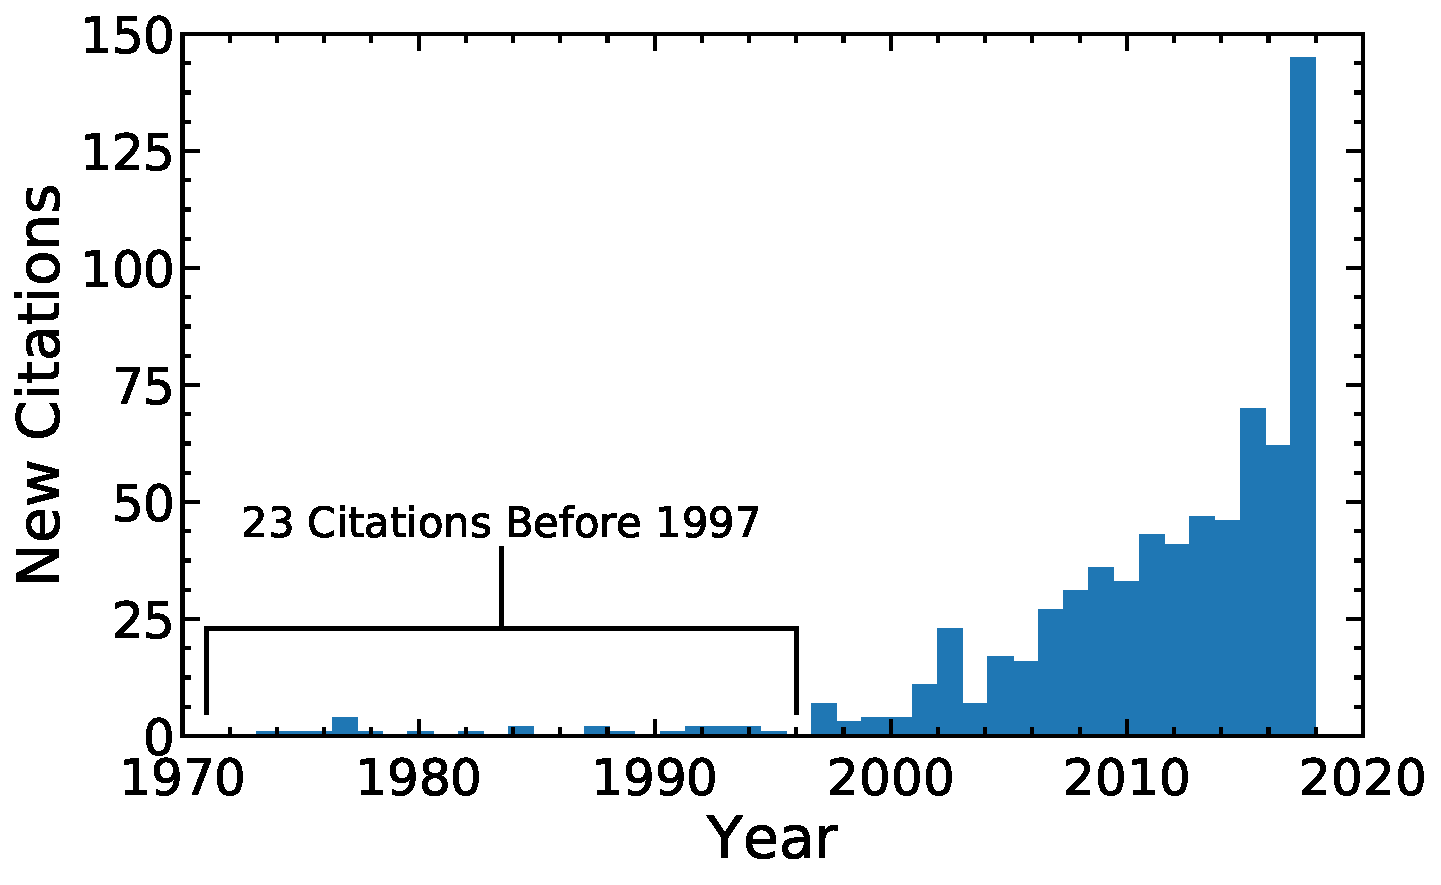
\includegraphics[width=0.8\textwidth]{./Figures/Polder1971Citations.pdf}
\caption{Timeline of citations of Polder and Van Hove's seminal work.\cite{Polder1971}}
\label{fig:Polder1971Citations}
\end{figure}
%
Polder and Van Hove's solution to NFRHT between half-spaces belongs to a class of solutions which are numerically exact for isotropic linear media. That is to say, no theoretical simplifications are required to derive their results and their method converges to the exact value of heat transfer in the correct numerical limit (such as increasing the number of terms in a truncated infinite sum or increasing the density of a mesh). The most common numerically exact methods involve dyadic Green's functions (DGFs),\cite{Joulain2005, Volokitin2007, Francoeur2008, Narayanaswamy2013a} spectral densities,\cite{Kruger2012} fluctuating surface currents/boundary element methods (BEM),\cite{Rodriguez2012} or thermal discrete dipole approximations (T-DDA),\cite{Edalatpour2014} each with its own advantages and limitations. These methods can again be broken into two classes of solutions: meshed and meshless solutions. DGF and spectral density solutions are most commonly meshless. They are best applied to geometries such as spheres, cylinders, and planes which have convenient bases in which to express eigenfunction expansions. BEM and T-DDA typically require surface and volume meshing, respectively. Their great advantage is that they are easily applied to arbitrary geometries; however, their computational time is often significantly greater than their meshless cousins. 

Despite having a number of theoretical frameworks to choose from, the frameworks themselves lack the immediately apparent insight that CRT can provide; their governing formulas are very abstract. To that end, a great deal of research has been directed towards determining explicit formulas for heat transfer in experimentally important thermal systems. Certain problems are best attacked using DGF and spectral density methods such as NFRHT in plane-plane, \cite{Polder1971} sphere-sphere, \cite{Narayanaswamy2008, Mackowski2008, Kruger2012, Czapla2017} and sphere-plane \cite{Kruger2011, Otey2011} configurations, where the electromagnetic fields are easily described by vector wave eigenfunction expansions. Thermal systems which do not yield to those methods often require meshed methods, such as BEM and T-DDA. Those methods have allowed investigations of cone-plane \cite{Rodriguez2013, Edalatpour2016} and cube-cube \cite{Edalatpour2014} configurations, among others. See Fig. \ref{fig:ExactMethods} for examples from the literature. In all cases presented, the characteristic lengths of at least one object were less than the thermal wavelength. 

\begin{figure}
\centering
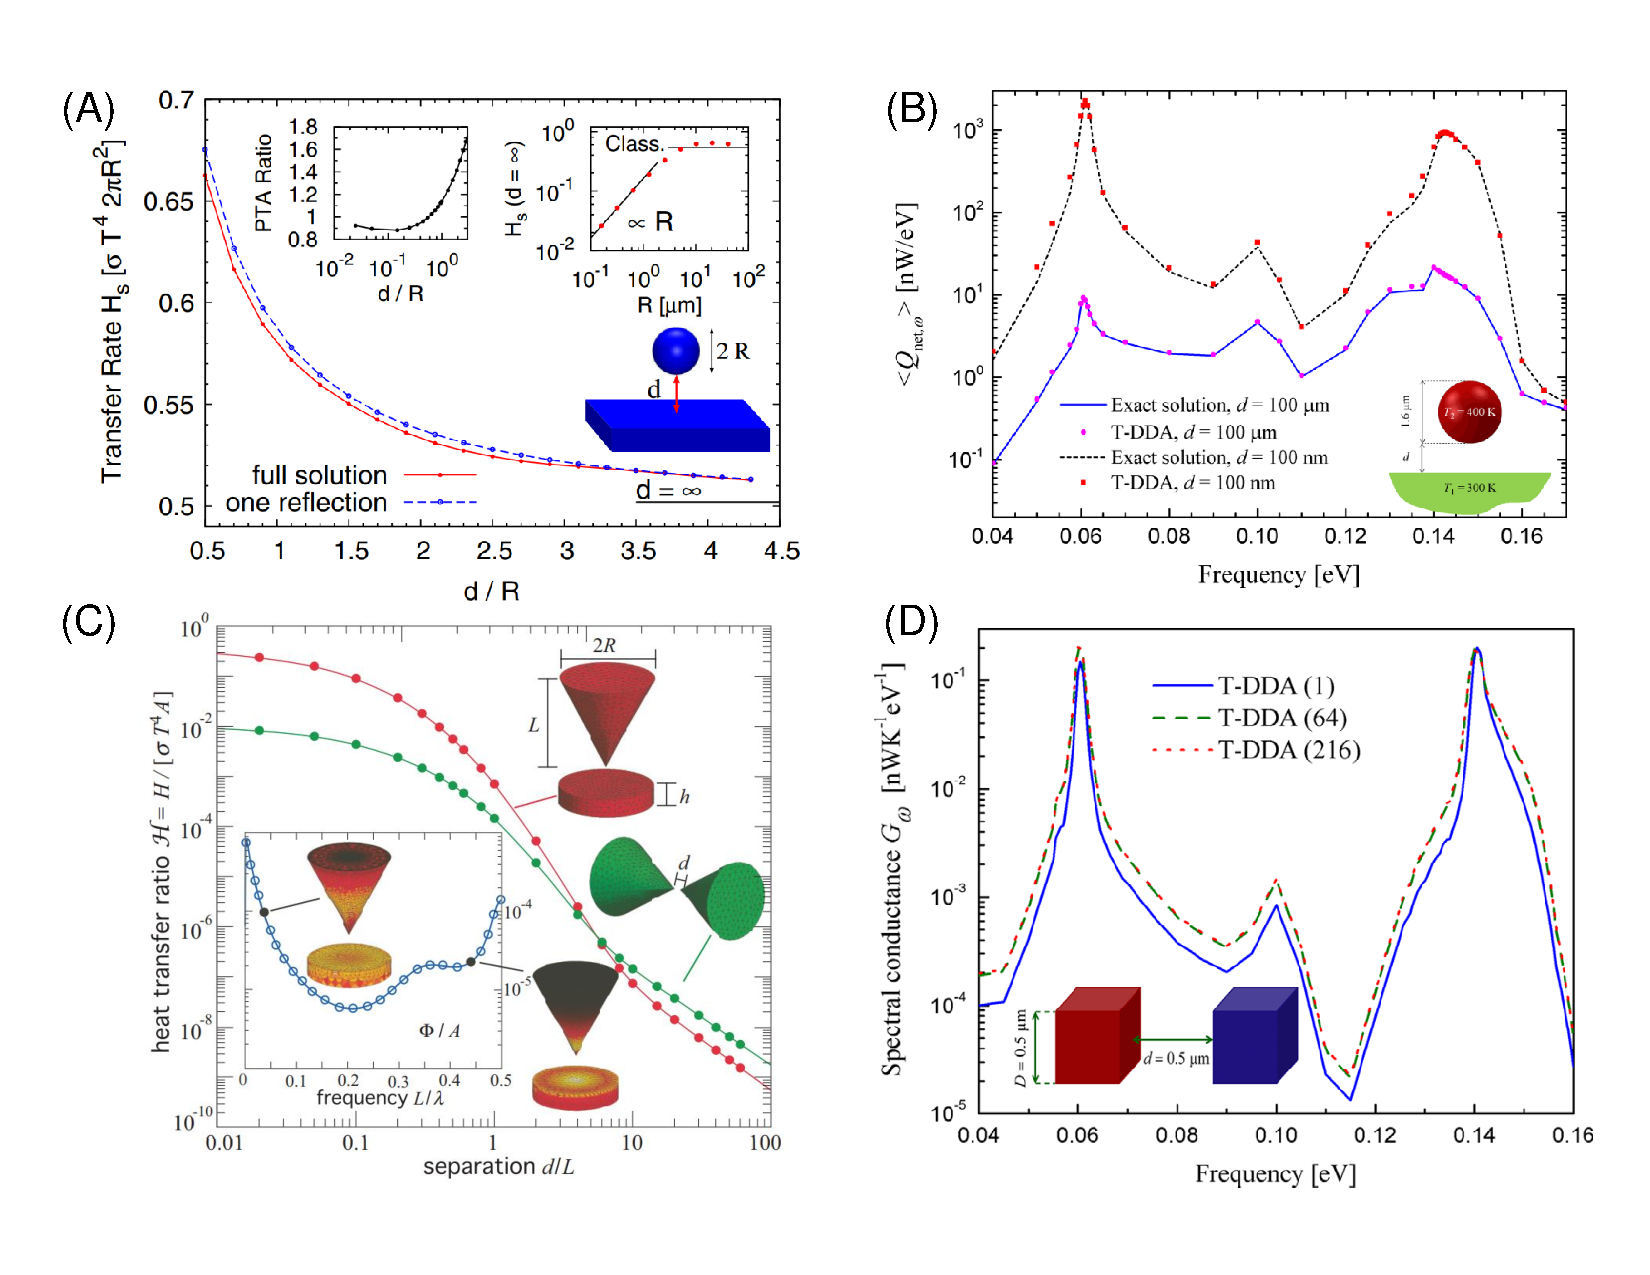
\includegraphics[width=\textwidth]{./Figures/ExactMethods.pdf}
\caption{\label{fig:ExactMethods}Selected NFRHT results from the literature. (A) Distance dependence of NFRHT in the sphere-plane configuration using spectral densities (labeled full solution).\cite{Kruger2011} (B) Frequency dependence of NFRHT in the sphere-plane configuration using DGFs (labeled exact solution) and T-DDA.\cite{Edalatpour2016} (C) Distance dependence of NFRHT in the cone-cone and cone-plane configurations using BEM.\cite{Rodriguez2013} (D) Frequency dependence of NFRHT in the cube-cube configuration using T-DDA.\cite{Edalatpour2014}}
\end{figure}


\subsection{Thermal Hyperbolic Metamaterials}
%
Optical metamaterials are a class of artificial materials which exhibit electromagnetic behavior not otherwise observed in nature, such as negative refractive index,\cite{Smith2004, Zhang2005, Soukoulis2007, Valentine2008} cloaking, \cite{Alu2005, Schurig2006, Cai2007, Valentine2009} and superlensing.\cite{Pendry2000, Fang2005, Smolyaninov2007, Zhang2008} Of particular interest are hyperbolic metamaterials (HMMs), materials whose permissible wavevector components form a hyperbolic isofrequency surface instead of the spherical surface found in typical isotropic materials. The simplest means of achieving HMM behavior is through layering different isotropic materials. When the layer thicknesses are much smaller than the free-space wavelength of light propagating through them, the entire nanocomposite can be viewed as a homogeneous material with hyperbolic effective optical properties.\cite{Halevi1999, Smith2003}

Hyperbolic metamaterials have found many uses in the field of near-field thermal radiative transfer. Appropriately designed HMMs have demonstrated the ability to tailor the spectrum of radiative transfer and to achieve super-Planckian heat transfer.\cite{Francoeur2011, Liu2011, Mason2011, Biehs2012, Guo2012, Guo2013, Liu2013} To date, this has mostly been achieved by using layered planar surfaces and computing the NFRHT using a DGF formalism.\cite{Biehs2007, Fu2009, Svetovoy2012} That configuration is attractive because the analytic solution to near-field thermal radiative transfer between two semi-infinite half spaces is well known, relatively straightforward to compute, and easily generalizes to include layered media.\cite{Polder1971, Francoeur2008, Francoeur2009, Song2016}

Figure \ref{fig:ExactMethods} depicts a typical numerical study of thermal HMMs.\cite{Guo2012a, Guo2013} Figure \ref{fig:ExactMethods}A shows two common methods of creating HMMs from linear, isotropic media. In this section, we focus on planar layered media. Figure \ref{fig:ExactMethods}B shows the spectrum of radiative transfer between two semi-infinite half spaces composed of alternating layers of silicon carbide and silicon dioxide. The left plot in Fig. \ref{fig:ExactMethods}B is obtained by integrating over the values of $k_{\rho}$ shown in the right plot. The main takeaway is that the contributions from high values of $k_{\rho}/k_{0}$, called high-k modes, are enabled by the hyperbolic optical properties of the half-spaces. 

HMMs composed of layered media are fundamentally limited in the extreme near-field. Mulet et al. showed that a particle exchanging thermal radiation with an object will only interact with the object to a depth comparable to the particle-object separation distance.\cite{Mulet2001} Considering any two layered objects to be made of an ensemble of particles, should the outermost layers become thicker than the separation distance, the near-field interaction should resemble NFRHT between two homogeneous objects composed of the outermost materials. This effect can lead to non-monotonic heat transfer with respect to distance.\cite{Esquivel-Sirvent2016}

\begin{figure}
\centering
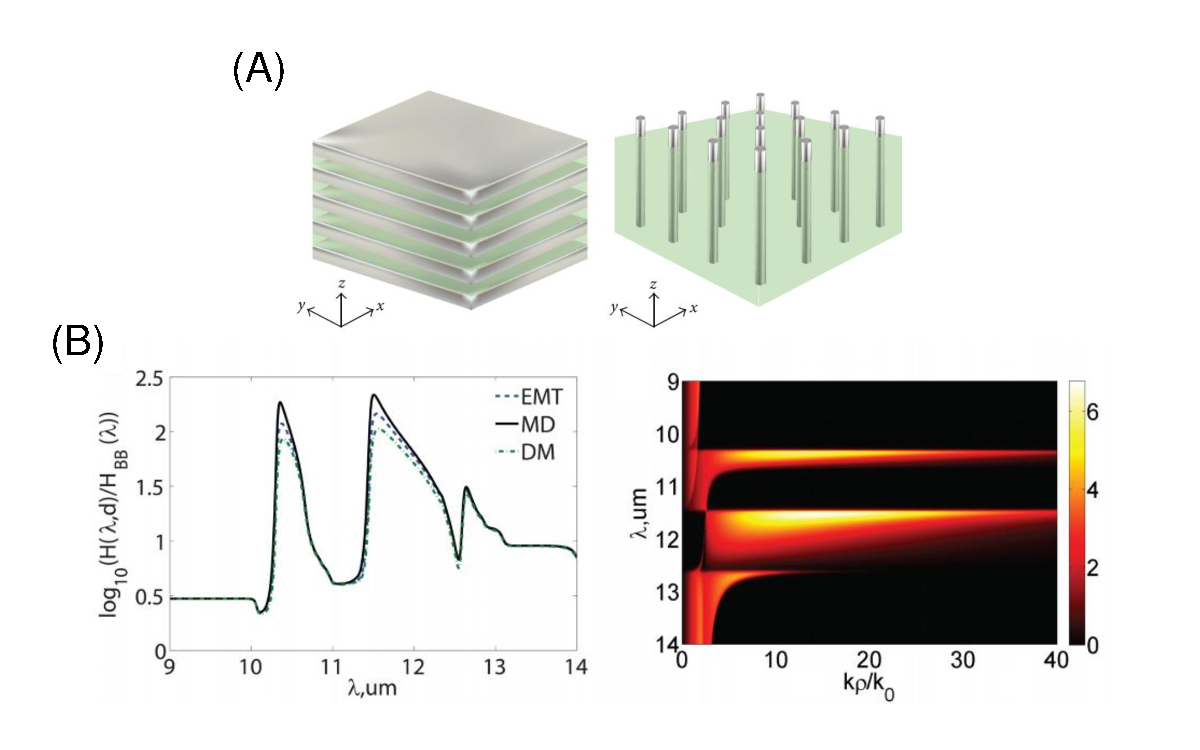
\includegraphics[width=\textwidth]{./Figures/HMM.pdf}
\caption{\label{fig:ExactMethods}(A) Schematic of two types of HMMs.\cite{Guo2012a} (B) Heat transfer between two layered semi-infinite half spaces composed of alternating layers of silicon carbide and silicon dioxide. The high-k modes are made possible by effective HMM optical properties.\cite{Guo2013}}
\end{figure}


\subsection{Experiments}
%
Compared to the great strides in theory made over the past decades, the experimental measurement of NFRHT is relatively immature. The oldest experiments involving NFRHT took place at between planar surfaces at cryogenic temperatures and relatively large gaps (10$^{2}$ \si{\micro\meter} to 10$^{3}$ \si{\micro\meter}).\cite{Cravalho1968, Domoto1970a} Though some modern work is still done at cryogenic temperatures\cite{Kralik2012} and/or using planar surfaces\cite{Kralik2012, Ghashami2018} (see Fig. \ref{fig:NFRHT_Experiments}C), most modern experiments occur at room temperature, and often do not involve two planar surfaces to avoid the difficulty in maintaining mutually parallel surfaces. Until the recent advances in NFRHT between MEMS devices\cite{Song2016, Cui2017, Fiorino2018} (see Fig. \ref{fig:NFRHT_Experiments}A), experiments measuring NFRHT in sub-micron gaps were performed in the microsphere-plane configuration (see Fig. \ref{fig:NFRHT_Experiments}B), much like the configurations used in Casimir and van der Waals force experiments.\cite{Lamoreaux1997, Mohideen1998, Roy1999, Harris2000} The rotational invariance of spheres, and to a lesser degree the small rotational variance of probes with rounded tips, removes the obstacle of maintaining parallel surfaces. A detailed critique of the microsphere-plane experimental configuration will be provided in Chapter \ref{ch:results}, based on the results of this dissertation.

\begin{figure}
\centering
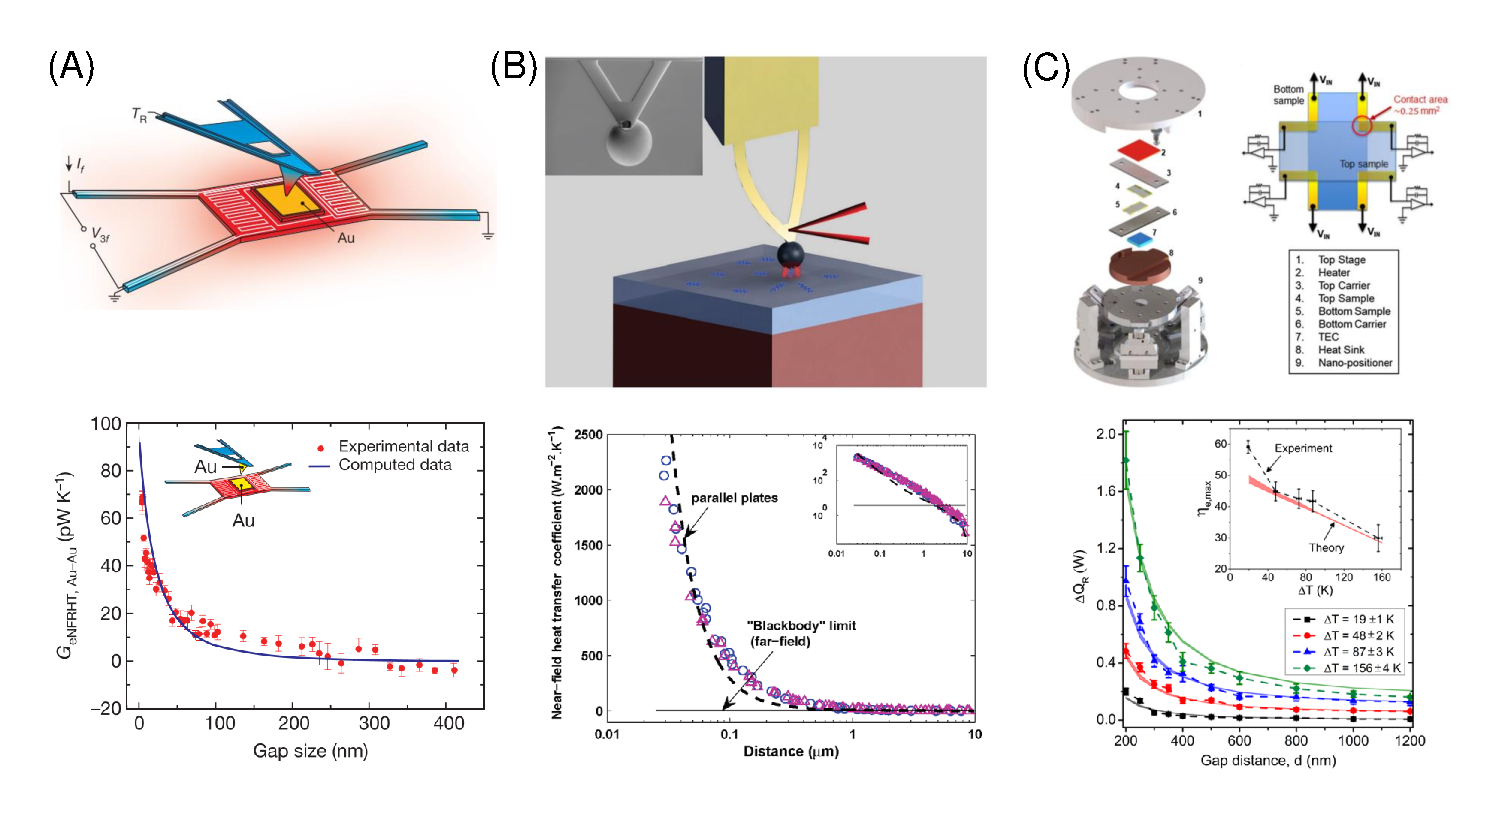
\includegraphics[width=\textwidth]{./Figures/NFRHT_Experiments.pdf}
\caption{\label{fig:NFRHT_Experiments}(A) NFRHT between a probe with a 300 \si{\nano\meter} radius spherical tip and a plane.\cite{Kim2015} (B) NFRHT between a sphere with a 50 \si{\micro\meter} or 100 \si{\micro\meter} radius and a plane.\cite{Shen2009} (C) NFRHT between two planar surfaces.\cite{Ghashami2018}}
\end{figure}


%\subsection{Open Questions}
%%
%Given the brief overview of NFRHT provided in this chapter, 
%
%What further geometries can be solved exactly?
%
%Extreme near-field, sub-Angstrom gaps. Radiation-condiction crossover, divergent bahviour of NFRHT isn't realistic, phonon tunneling, spatial dispersion
%
%Computation problems in many-body problems
%
%immature experiments compared to theory 
%
%Actual technologies


\section{Purpose and Outline of This Work}
%
The goal of this work is simple: to provide explicit formulas which completely describe a thermal system consisting of layered spheres in a linear chain. While this system has been previously investigated for two spheres,\cite{Narayanaswamy2008, Mackowski2008, Sasihithlu2011, Sasihithlu2011a, Kruger2012, Sasihithlu2012, Sasihithlu2014} light scattering,\cite{Fuller1988, Li2003, Wei2004, Chen2006, Lee2013} and radiative transfer in the dipole limit,\cite{Ben-Abdallah2011, Dong2017a, Kathmann2018} it has not yet been rigorously characterized for NFRHT between spheres of arbitrary size, with or without spherical layers. The key results of this work are numerically exact expressions for NFRHT between pairs of spheres in a linear chain, and between any sphere in a chain and its environment. The results of this dissertation allow for a rigorous critique of past sphere-plane experiments, focusing on how sphere-environment heat transfer is typically handled. Using the analysis, I provide a guidelines for designing future experiments between two spheres which ensure accurate interpretation of results. 

The outline of the dissertation is as follows: Chapter \ref{ch:Electromagnetism} builds up the basics of electromagnetic theory necessary to solve this problem. Starting from Maxwell's equations, the vector Helmholtz (wave) equation is derived for electric and magnetic fields in the Fourier domain. The Helmholtz equation is the governing equation for this work, and must be inverted to solve for the electric and magnetic fields, and ultimately radiative heat transfer. As part of that equation, knowledge of the optical properties of materials is required. I present a simple derivation of the Lorentz model for dielectric function and demonstrate how the model can be fit to a particular material by looking at a case study involving polydimethylsiloxane. Chapter \ref{ch:DGFs} covers the DGF formalism which will be employed to solve the problem. A general geometry for the formalism is established for an arbitrary number of objects embedded in a large free-space region. I show how DGFs can be used to isolate the contributions of fluctuating charges in each object to the electric and magnetic field at any other point. This will prove crucial to evaluating heat transfer between objects. I then go on to define the Poynting vector and describe the fluctuation-dissipation theorem, two important pieces to the puzzle. From there, I define a Landauer-like formula for radiative transfer that separates the temperature dependence from the geometric and configuration dependencies, which are contained in a transmissivity function for energy transfer. Crucially, the volumetric processes of emission and absorption are converted into surface integrals, which drastically simplifies computation. Finally, as a demonstration, I use the DGF formalism to compute NFRHT between planar media. Chapter \ref{ch:model} applies the DGF formalism to the case of coated spheres in a chain. The necessary eigenfunctions, the vector spherical waves, are provided which allow the DGFs of the system to be defined. The chain is analyzed and sphere-sphere and sphere-environment heat transfer formulas are provided. Chapter \ref{ch:results} serves to validate the results of this dissertation against BEM and T-DDA models before analyzing a few interesting cases. Those cases are NFRHT between two dielectric coated metal spheres and two dielectric coated dielectric spheres. I also propose a hypothetical two sphere NFRHT experiment and analyze the thermal model required to achieve accurate results. Chapter \ref{ch:Summary} summarizes my contributions to the field of NFRHT and suggests future areas of research.

Additionally, I supply a number of appendices for convenience of reference. Appendix \ref{ap:FresnelCoefficients} discusses the Fresnel reflection coefficients and provides their formulas. Appendix \ref{ap:CRT} is a brief summary of the common formulas used to compute CRT between two engineering surfaces. Appendix \ref{ap:Math} provides a number of mathematical formulas and relations useful throughout this work. Appendix \ref{ap:MieCoefficients} provides formulas for the effective Mie coefficients of layered media. Appendix \ref{ap:SolutionToLinearSystem} explains how to compute the scattered field coefficients that arise in sphere-sphere NFRHT calculations. Appendix \ref{ap:SCUFFEM} details the steps required to perform a NFRHT simulation using \textsc{scuff-em}.% Done X
\chapter[Fundamentals of Electromagnetism][Fundamentals of Electromagnetism]{Fundamentals of Electromagnetism} \label{ch:Electromagnetism}
%
\section{Outline of Chapter}
%
In this chapter, I will cover the fundamental concepts from electromagnetism which will prove crucial for understanding this work. Starting from Maxwell's equations, I will derive the vector Helmholtz equation in the Fourier domain for linear isotropic media; the vector Helmholtz equation is the governing equation for this work. Next, I will derive a common model for the optical properties of dielectrics, the Lorentz model, and will discuss my work using reflection measurements to fit the Lorentz model for the polymer polydimethylsiloxane (PDMS).


\section{Maxwell's Equations} \label{sec:MaxwellEquations}
%
Maxwell's equations describe the origin and evolution of electric and magnetic fields, which are critical when determining radiative heat transfer. These fields can be created by charges, currents, or changes in the fields themselves. In the time domain, the macroscopic set of equations at position $\boldsymbol{r}$ and time $t$ are given by
\begin{subequations}
\begin{align}
\boldsymbol{\nabla} \cdot \widehat{\boldsymbol{D}}(\boldsymbol{r}, t) &= \widehat{\rho}_e(\boldsymbol{r}, t) \label{eq:ElectricDivergence}
\\
\boldsymbol{\nabla} \cdot \widehat{\boldsymbol{B}}(\boldsymbol{r}, t) &= \widehat{\rho}_m(\boldsymbol{r}, t) \label{eq:MagneticDivergence}
\\
\boldsymbol{\nabla} \times \widehat{\boldsymbol{E}}(\boldsymbol{r}, t) &= - \frac{\partial \widehat{\boldsymbol{B}}(\boldsymbol{r}, t)}{\partial t} - \widehat{\boldsymbol{J}}^m(\boldsymbol{r}, t) \label{eq:MaxwellCurlElectric1}
\\
\boldsymbol{\nabla} \times \widehat{\boldsymbol{H}}(\boldsymbol{r}, t) &= \frac{\partial \widehat{\boldsymbol{D}}(\boldsymbol{r}, t)}{\partial t} + \widehat{\boldsymbol{J}}^e(\boldsymbol{r}, t) \label{eq:MaxwellCurlMagnetic1}
\end{align}
\end{subequations}
%
where $\boldsymbol{\nabla} \cdot \left( \cdot \right)$ and $\boldsymbol{\nabla} \times \left( \cdot \right)$ denote the divergence and curl operators; $\widehat{\boldsymbol{D}}$, $\widehat{\boldsymbol{E}}$, $\widehat{\boldsymbol{B}}$, and $\widehat{\boldsymbol{H}}$ are the displacement, electric, magnetic flux density, and magnetic fields respectively; $\widehat{\rho}_e$ and $\widehat{\rho}_m$ are the electric and magnetic current densities; and $\widehat{\boldsymbol{J}}^e$ and $\widehat{\boldsymbol{J}}^m$ are the electric and magnetic free current densities. The hat over various symbols indicates the quantity is expressed in the time domain.

The version of Maxwell equations presented above has a number of magnetic terms added to the traditionally presented equations.\cite{Jackson1998} The terms are added to enforce symmetry between the electric and magnetic equations, but ultimately have little bearing on results, since the added terms can be set to zero later to recover the more traditional form of the equations. 

It will prove advantageous to work with Maxwell's equations in their time harmonic form, i.e. assume $\widehat{\boldsymbol{F}}(\boldsymbol{r}, t) = \mathrm{Re}[{\boldsymbol{F}}(\boldsymbol{r}) e^{-i \omega t}]$, where $\widehat{\boldsymbol{F}}$ can be $\widehat{\boldsymbol{D}}$, $\widehat{\boldsymbol{E}}$, $\widehat{\boldsymbol{B}}$, or $\widehat{\boldsymbol{H}}$, $\omega$ is the angular frequency, and $\mathrm{Re}(\cdot)$ indicates the real component of a complex number. Focusing now on Eqs. \ref {eq:MaxwellCurlElectric1} and \ref {eq:MaxwellCurlMagnetic1} and moving from the time domain to the Fourier domain, we get
%
\begin{subequations}
\begin{align}
\boldsymbol{\nabla} \times \boldsymbol{E}(\boldsymbol{r}) &= i \omega \boldsymbol{B}(\boldsymbol{r}) - \boldsymbol{J}^m(\boldsymbol{r}) \label{eq:MaxwellCurlElectric2}
\\
\boldsymbol{\nabla} \times \boldsymbol{H}(\boldsymbol{r}) &= - i \omega \boldsymbol{D}(\boldsymbol{r}) + \boldsymbol{J}^e(\boldsymbol{r}) \label{eq:MaxwellCurlMagnetic2}
\end{align}
\end{subequations}

In order to proceed, we will reduce the number of unknown fields in Maxwell's equations to two: $\boldsymbol{E}$ and $\boldsymbol{H}$. The displacement and magnetic flux density fields are given, by definition, as
%
\begin{subequations}
\begin{align}
\boldsymbol{D}(\boldsymbol{r}) &= \varepsilon_{0} \left( \boldsymbol{E} + \varepsilon_{0}^{-1} \boldsymbol{P} \right)
\\
\boldsymbol{B}(\boldsymbol{r}) &= \mu_{0} \left( \boldsymbol{H} + \boldsymbol{M} \right)
\end{align}
\end{subequations}
%
where $\boldsymbol{P}$ and $\boldsymbol{M}$ are the polarization and magnetization fields and $\varepsilon_{0}$ and $\mu_{0}$ are the permittivity and permeability of free space. The free space permittivity and permeability are constants which are related to the speed of light in vacuum, $c$, by $c = 1/\sqrt{\varepsilon_{0} \mu_{0}}$.

Rather annoyingly, at least in the my field, the polarization and magnetization fields lack the apparent symmetry that Maxwell's equations deserve. But all is not lost. In this work, I will work exclusively with linear, isotropic medium which have constitutive relations 
%
\begin{subequations}
\begin{align}
\varepsilon_{0}^{-1} \boldsymbol{P} &= \chi_{e} \boldsymbol{E} \label{eq:Polarization}
\\
\boldsymbol{M} &= \chi_{m} \boldsymbol{H}
\end{align}
\end{subequations}

Here, $\chi_{e}$ and $\chi_{m}$ are the electric and magnetic susceptibilities, which are themselves defined as
%
\begin{subequations}
\begin{align}
\chi_{e} &= \varepsilon - 1 \label{eq:ElectricSusceptibility}
\\
\chi_{m} &= \mu - 1
\end{align}
\end{subequations}
%
in linear media. $\varepsilon$ and $\mu$ are the relative permittivity and permeability, respectively. $\varepsilon$ and $\mu$ are often written with an $r$ subscript (to indicate relative) in other works. The unsubscripted variables are then commonly used to denote the products of the relative and free space variables. But in this work, because we will rarely need the product of the relative and free space variables, that quantity will be given no symbol, and the other quantities will be defined as described above. $\varepsilon$ is also commonly called the dielectric function, and is explored thoroughly in Section \ref{sec:OpticalProperties}.

Now that all the groundwork has been laid, we can simplify Eqs. \ref{eq:MaxwellCurlElectric2} and \ref{eq:MaxwellCurlMagnetic2} to include only the electric and magnetic fields. The simplification yields
%
\begin{subequations}
\begin{align}
\boldsymbol{\nabla} \times \boldsymbol{E}(\boldsymbol{r}) &= i \omega \mu \mu_{0} \boldsymbol{H}(\boldsymbol{r}) - \boldsymbol{J}^m(\boldsymbol{r}) \label{eq:MaxwellCurlElectric3}
\\
\boldsymbol{\nabla} \times \boldsymbol{H}(\boldsymbol{r}) &= - i \omega \varepsilon \varepsilon_{0} \boldsymbol{E}(\boldsymbol{r}) + \boldsymbol{J}^e(\boldsymbol{r}) \label{eq:MaxwellCurlMagnetic3}
\end{align}
\end{subequations}

Finally, we can substitute Eqs. \ref{eq:MaxwellCurlElectric3} and \ref{eq:MaxwellCurlMagnetic3} into one another to achieve
\begin{subequations}
\begin{align}
\boldsymbol{\nabla} \times \boldsymbol{\nabla} \times \boldsymbol{H}(\boldsymbol{r}) - k^{2} \boldsymbol{H}(\boldsymbol{r}) &= i \omega \varepsilon \varepsilon_{0} \boldsymbol{J}^m(\boldsymbol{r}) + \boldsymbol{\nabla} \times  \boldsymbol{J}^e(\boldsymbol{r}) \label{eq:MaxwellCurlElectric4}
\\
\boldsymbol{\nabla} \times \boldsymbol{\nabla} \times \boldsymbol{E}(\boldsymbol{r}) - k^{2} \boldsymbol{E}(\boldsymbol{r})&= i \omega \mu \mu_{0} \boldsymbol{J}^e(\boldsymbol{r}) - \boldsymbol{\nabla} \times \boldsymbol{J}^m(\boldsymbol{r}) \label{eq:MaxwellCurlMagnetic4}
\end{align}
\end{subequations}
%
where $k = (\omega/c) \sqrt{\varepsilon \mu}$ is the wavevector. Eqs. \ref{eq:MaxwellCurlElectric4} and \ref{eq:MaxwellCurlMagnetic4} are examples of the inhomogeneous vector Helmholtz equation. The challenge now is to invert the equations to obtain $\boldsymbol{E}$ and $\boldsymbol{H}$. This can be achieved using dyadic Green's functions, which will be discussed in Chapter \ref{ch:DGFs}.


\section{Optical Properties of Materials} \label{sec:OpticalProperties}

\subsection{Overview}
%
When discussing the optical properties of linear isotropic media, there are three crucial unitless parameters: the dielectric function, relative permeability, and refractive index. In general, all three quantities are complex-valued and frequency-dependent. The dielectric function (relative permeability) is a measure of a material's degree of polarization (magnetization) under the influence of an externally applied electric (magnetic) field. The refractive index describes how light propagates through a medium. Its real and imaginary parts correspond to speed and dissipation of light as it passes through the medium, respectively. The three quantities are related to one another by
%
\begin{equation}
n_{c} = \sqrt{\varepsilon \mu} = n + i \kappa
\end{equation}
%
where $n_{c}$ is the complex refractive index and $n$ and $\kappa$ are the real and imaginary components of $n_{c}$. $n$ is the refractive index and $\kappa$ is the extinction coefficient. In the infrared portion of the electromagnetic spectrum where this work is focused, most materials do not exhibit magnetic behavior ($\mu \approx 1$). Thus, the subsequent discussion in this section will focus on the dielectric function. 


\subsection{Dielectric Function}
%
\begin{figure}
\centering
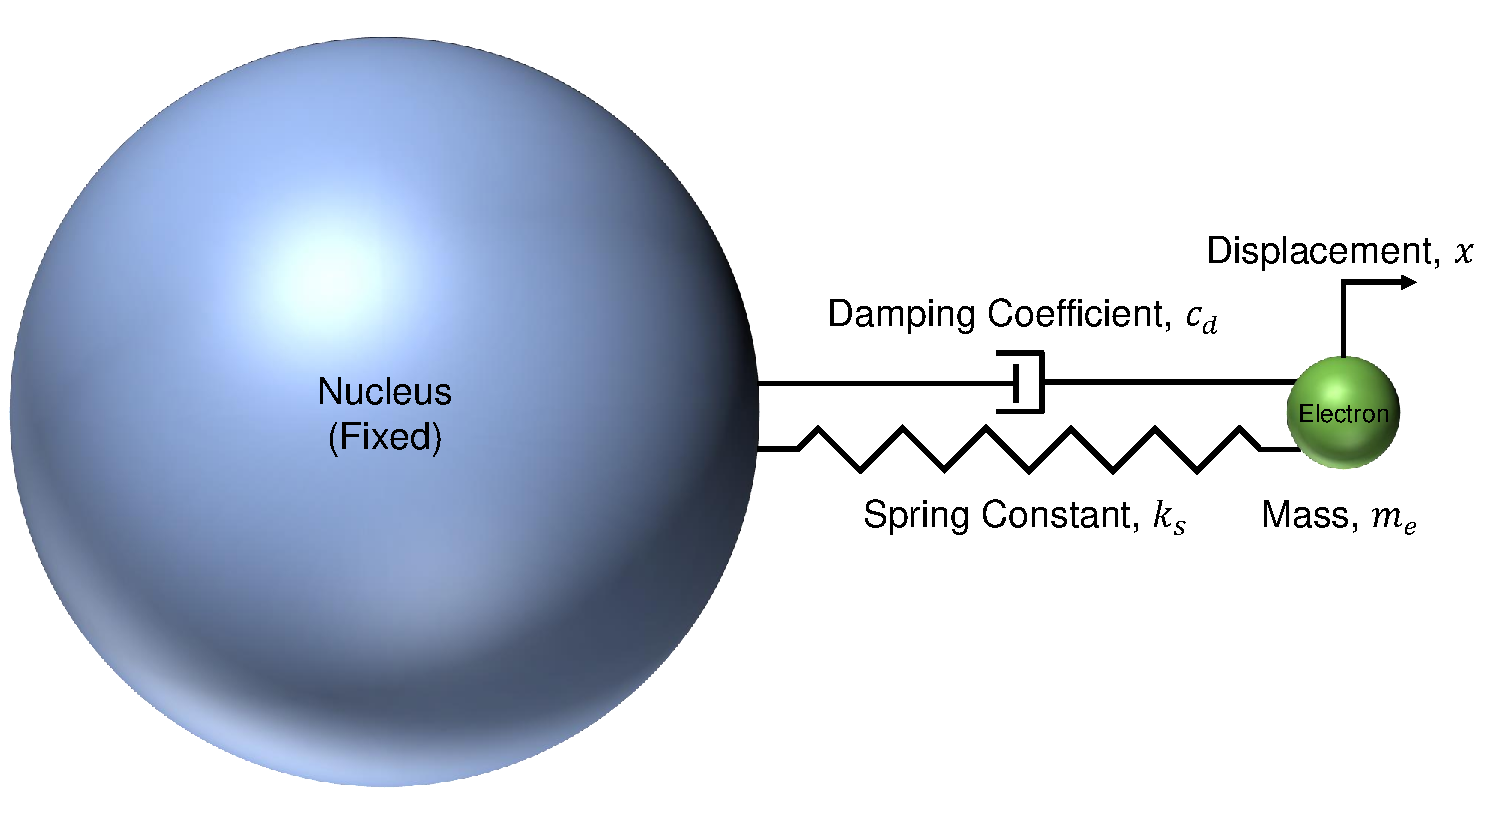
\includegraphics[width=0.8\textwidth]{./Figures/SpringMassDamper.pdf}
\caption{\label{fig:SpringMassDamper}Conceptual diagram of the spring-mass-damper system of an electron bound to its nucleus.}
\end{figure}
%
To derive a model for the dielectric function, we will examine the dynamics of a bound electron around a nucleus, which can be approximated by a spring-mass-damper system (see Fig. \ref{fig:SpringMassDamper}). In the time domain, the governing equation of such a system is
%
\begin{equation}
\widehat{\boldsymbol{F}} = m_{e} \ddot{\widehat{\boldsymbol{x}}} + c_{d} \dot{\widehat{\boldsymbol{x}}} + k_{s} \widehat{\boldsymbol{x}}
\end{equation}
%
where a dot indicates a time derivative. Again assuming a time harmonic response and moving into the Fourier domain, the equivalent equation is
%
\begin{equation}
\boldsymbol{F} = \left( - \omega^{2} m_{e} - i \omega c_{d} + k_{s} \right) \boldsymbol{x}
\end{equation}

Further simplification can be made by using insight from spring-mass damper systems. The undamped resonant frequency and damping factor, $\omega_{0}$ and $\zeta$, are defined as $\omega_{0} = \sqrt{k_{s}/m_{e}}$ and $\zeta = c_{d}/(2\sqrt{k_{s}m_{e}})$, respectively. Substituting in accordingly, we get
%
\begin{equation}
\boldsymbol{F} = m_{e} \left( - \omega^{2} - i2 \omega \omega_{0} \zeta + \omega_{0}^{2} \right) \boldsymbol{x}
\end{equation}

Next, we must use insight from electromagnetism. First, the force on a particle in a uniform electric field is $\boldsymbol{F} = q_{e} \boldsymbol{E}$, where $q_{e}$ is the charge of the particle. Further, the polarization field is related to the displacement by $\boldsymbol{P} = N_{e} q_{e} \boldsymbol{x}$, where $N_{e}$ is the average number of electrons in a unit volume. These facts, in conjunction with Eqs. \ref{eq:Polarization} and \ref{eq:ElectricSusceptibility}, yield
%
\begin{equation}
\boldsymbol{x} = \frac{\varepsilon_{0} \left( \varepsilon - 1 \right)}{N q_{e}} \boldsymbol{E}
\end{equation}

Putting everything together and solving for $\varepsilon$, we arrive at
%
\begin{equation}
\varepsilon = 1 + \frac{S}{1 - \left( \frac{\omega}{\omega_{0}} \right)^{2} - i \Gamma \left( \frac{\omega}{\omega_{0}} \right)}
\end{equation}
%
where $\Gamma = 2 \zeta$ and $S = N_{e} q_{e}^{2} / (w_{0}^{2} m_{e} \varepsilon_{0})$. This derived model is the simplest form of the Lorentz oscillator model. In reality, not all materials are composed of only identical nuclei and bound electrons like Fig. \ref{fig:SpringMassDamper} depicts. Many common dielectrics are composed of atoms arranged with multiple covalent bonds, each with its own resonant frequency. Thus, its is not unreasonable to expect that such a material's dielectric function would reflect the multiple resonances. These multiple resonances are accounted for by summing over the necessary number of oscillators
%
\begin{equation}
\varepsilon = \varepsilon_{\infty} + \sum_{j=1}^{N_{\mathrm{max}}} \left[ \frac{S_{j}}{1 - \left( \frac{\omega}{\omega_{0,j}} \right)^{2} - i \Gamma_{j} \left( \frac{\omega}{\omega_{0,j}} \right)} \right]
\end{equation}

The constant value of 1 was replaced by $\varepsilon_{\infty}$ because researchers often look at only a portion of the electromagnetic spectrum. Any oscillators with resonant frequencies much higher than the portion of the spectrum being examined manifest as an additional offset. For example, the parameters of a Lorentz model for polymethylmethacrylate (PMMA) are shown in Table. \ref{tab:PMMALorentzModel}. The Lorentz oscillator model is just one among many models for the dielectric function. Other common models are listed in Table \ref{tab:DielectricFunctionModels}.

\begin{table}
	\caption{\label{tab:PMMALorentzModel} Oscillator parameters determined to reproduce the dielectric function of PMMA.\cite{Tsuda2018} Unlisted is $\epsilon_{\infty}$ = $2.162$.}
	\begin{center}
		\renewcommand{\arraystretch}{1.15}
		\setlength{\tabcolsep}{0.10cm}
		\begin{tabular}{llllllllll}
			\hline 
			\hline
			\multicolumn{1}{c}{$j$} &
			\multicolumn{1}{c}{$\hbar \omega_{0}$ (eV)} & \multicolumn{1}{c}{$\lambda_{0}$ (\si{\micro\meter})} &
			\multicolumn{1}{c}{$S$} &
			\multicolumn{1}{c}{$\Gamma$} &
			\multicolumn{1}{c}{$j$} &
			\multicolumn{1}{c}{$\hbar \omega_{0}$ (eV)} & \multicolumn{1}{c}{$\lambda_{0}$ (\si{\micro\meter})} &
			\multicolumn{1}{c}{$S$} &
			\multicolumn{1}{c}{$\Gamma$} \\ 	
			\hline 
			%
			1 & 0.09327 & 13.29 & 3.18$ \times 10^{-3}$ & 0.01815 & 13 & 0.1688 & 7.345 & 1.09$ \times 10^{-3}$ & 0.03083 \\
			2 & 0.1002 & 12.37 & 6.94$ \times 10^{-4}$ & 0.01919 & 14 & 0.1720 & 7.207 & 1.07$ \times 10^{-3}$ & 0.01139 \\
			3 & 0.1023 & 12.12 & 1.13$ \times 10^{-4}$ & 0.005102 & 15 & 0.1779 & 6.970 & 1.34$ \times 10^{-3}$ & 0.007360 \\
			4 & 0.1045 & 11.86 & 2.86$ \times 10^{-3}$ & 0.02739 & 16 & 0.1799 & 6.894 & 4.11$ \times 10^{-3}$ & 0.01734 \\
			5 & 0.1133 & 10.94 & 1.68$ \times 10^{-3}$ & 0.03556 & 17 & 0.1837 & 6.748 & 2.12$ \times 10^{-3}$ & 0.01294 \\
			6 & 0.1197 & 10.36 & 3.94$ \times 10^{-3}$ & 0.02766 & 18 & 0.2145 & 5.7780 & 1.56$ \times 10^{-2}$ & 0.005433 \\
			7 & 0.1227 & 10.11 & 2.79$ \times 10^{-3}$ & 0.01483 & 19 & 0.3522 & 3.520 & 6.66$ \times 10^{-5}$ & 0.005393 \\
			8 & 0.1322 & 9.38 & 1.10$ \times 10^{-3}$ & 0.01272 & 20 & 0.3621 & 3.424 & 8.42$ \times 10^{-4}$ & 0.02086 \\
			9 & 0.1425 & 8.700 & 2.92$ \times 10^{-2}$ & 0.02708 & 21 & 0.3658 & 3.389 & 6.60$ \times 10^{-4}$ & 0.006372 \\
			10 & 0.1476 & 8.401 & 1.04$ \times 10^{-2}$ & 0.01858 & 22 & 0.3717 & 3.336 & 9.53$ \times 10^{-4}$ & 0.01224 \\
			11 & 0.1539 & 8.056 & 6.64$ \times 10^{-3}$ & 0.01722 & 23 & 0.4265 & 2.907 & 4.15$ \times 10^{-5}$ & 0.009852 \\
			12 & 0.1574 & 7.877 & 5.49$ \times 10^{-3}$ & 0.01942 &  &  &  &  &  \\
			\hline
			\hline
		\end{tabular} 
	\end{center}
\end{table}

\begin{table}
	\caption{\label{tab:DielectricFunctionModels}Common dielectric function models, presented in terms of angular frequency. $A$, $S$, $\omega_{0}$, $\Gamma$, $\varepsilon_{\infty}$, and $\omega_{p}$ are model parameters that must be determined for a given material.}
	\begin{center}
		\renewcommand{\arraystretch}{1.15}
		\setlength{\tabcolsep}{0.10cm}
		\begin{tabular}{llllllll}
			\hline 
			\multicolumn{1}{c}{Name} &
			\multicolumn{1}{c}{Model} & 
			\multicolumn{1}{c}{Applicability} \\
			\hline
			%
			Cauchy & $\varepsilon(\omega) = \left[ \sum_{j=0}^{N_{\mathrm{max}}} A_{j} \omega^{2j} \right]^{2}$ & Glassy Dielectrics \\
			Sellmeier & $\varepsilon(\omega) = \varepsilon_\infty + \sum_{j=1}^{N_{\mathrm{max}}} \left[ \frac{S_{j} }{1 - ( \omega / \omega_{0,j} )^{2} } \right]$ & Glassy Dielectrics \\
			Lorentz & $\varepsilon(\omega) = \varepsilon_\infty + \sum_{j=1}^{N_{\mathrm{max}}} \left[ \frac{S_{j} }{1 - ( \omega / \omega_{0,j} )^{2} -  i \Gamma_{j} (\omega / \omega_{0,j} ) } \right]$ & Crystalline Dielectrics \\
			Brendel-Bormann & See Ref. \citenum{Brendel1992}. & Amorphous Dielectrics \\
			Causal Voigt & See Ref. \citenum{DeSousaMeneses2005}. & Amorphous Dielectrics \\
			Drude & $\varepsilon(\omega) = 1 - \frac{\omega_p^2}{\left( \omega^2 +  i \Gamma \omega \right)}$ & Metals \\
			\hline
		\end{tabular} 
	\end{center}
\end{table}


\subsection{Method of Determining Dielectric Function}
%
Several methods of determining the dielectric function of a material exist in the literature, including as refractometry,\cite{Burnett2016} ellipsometry,\cite{Jellison1993} and reflectometry using Kramers-Kronig analysis.\cite{Roessler1965, Roessler1965a} In this section, I will explain my work, performed by Srinivasan, Czapla, Mayo, and Narayanaswamy (henceforth Srinivasan et al.), which focused on extracting the dielectric function of polydimethylsiloxane (PDMS) from reflection measurements by fitting a Lorentz model.\cite{Srinivasan2016} PDMS is a silicone elastomer which has a diverse set of applications ranging from MEMS\cite{Streque2010} and microfluidic devices\cite{Fujii2002, Lamberti2015, You2015} to surfactant\cite{Laubie2013} and antifoamer technologies.\cite{Owen2012}  It is well-known that PDMS is highly transmissive between 0.4 \si{\micro\meter} and 1.8 \si{\micro\meter}, making it attractive for optical waveguide communication and optofluidic applications.\cite{Mata2005, Psaltis2006, Cai2008, Cai2010, Cai2013} At the time Ref. \citenum{Srinivasan2016} was published, the complex refractive index of the solid form of PDMS had previously been reported only for visible to near-infrared wavelengths\cite{Spaeth1997, Cardenas-Valencia2006, Kopetz2007, Schneider2009, Cai2010, Cai2013, Kacik2014} and for wavelengths in the far-infrared or longer.\cite{Podzorov2008, Wang2012a, Khodasevych2012, Headland2015} A liquid form of PDMS was investigated by Querry in the range from 0.8 \si{\micro\meter} to 55.6 \si{\micro\meter}.\cite{Querry1987} Since the publication of Ref. \citenum{Srinivasan2016}, Motaharifar et al. also examined the infrared optical properties of PDMS.\cite{Motaharifar2018}

\begin{figure}
\centering
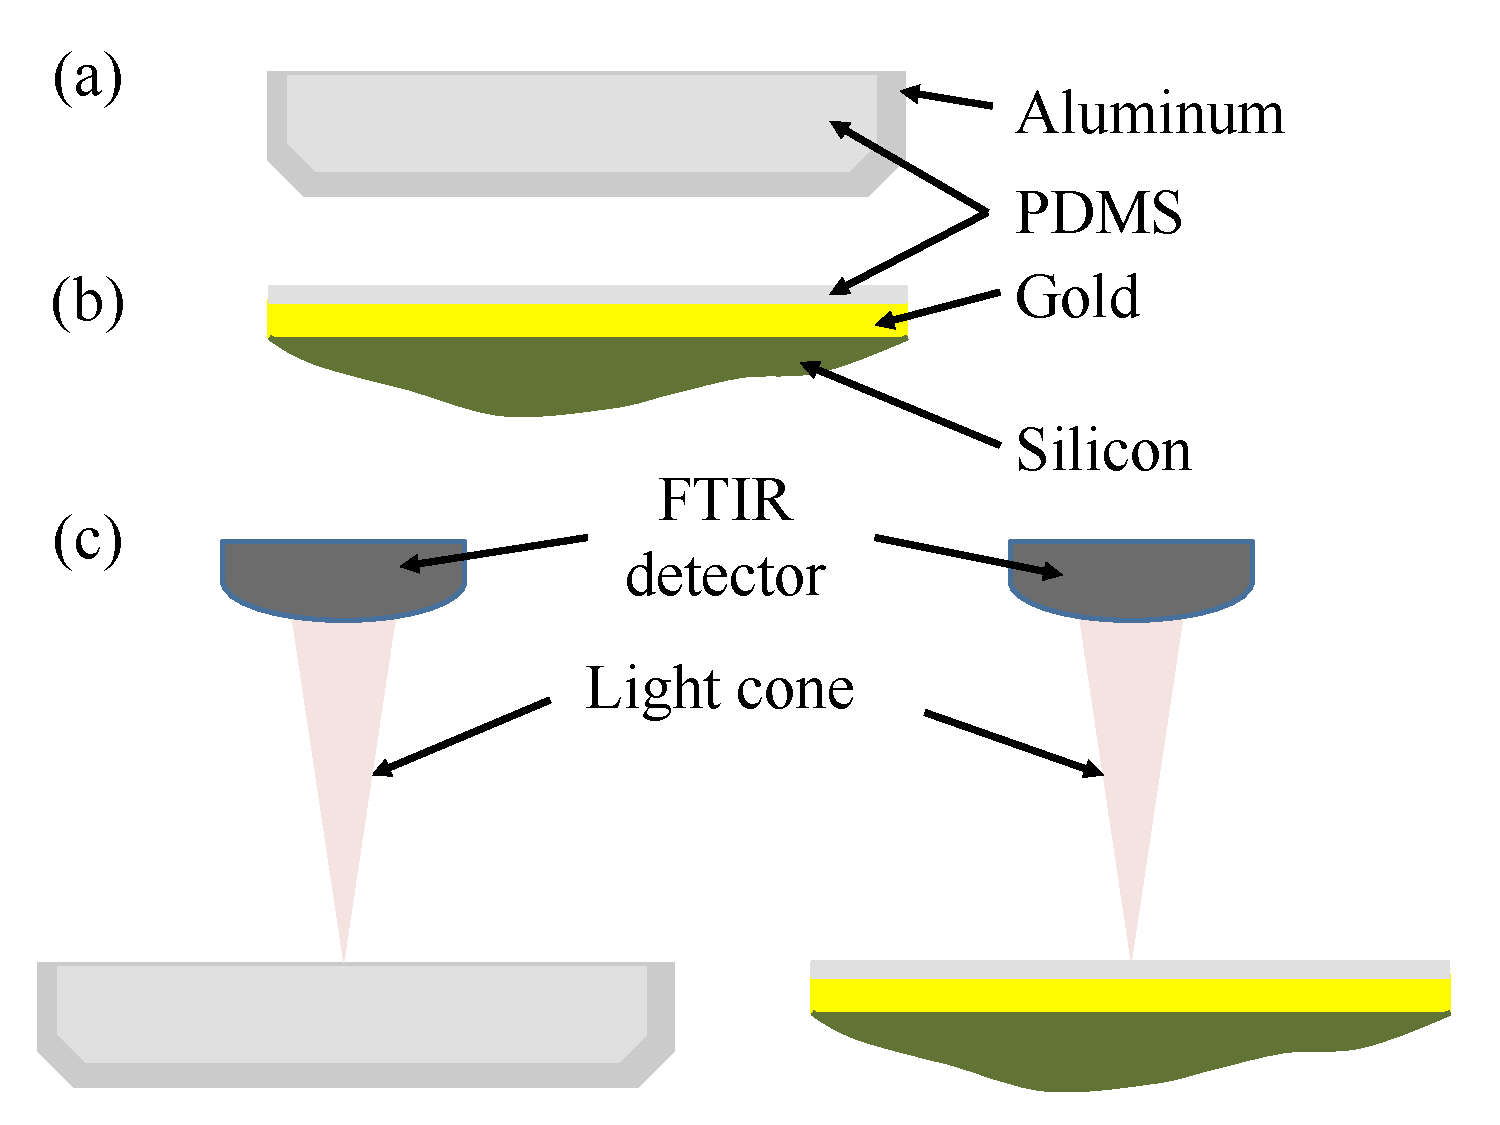
\includegraphics[width=0.8\textwidth]{./Figures/PDMS_Geometry.pdf}
\caption{\label{fig:PDMS_Geometry}(a) Geometry of bulk PDMS samples prepared in aluminum dishes. (b) PDMS thin film on top of gold coated silicon substrate. (c) Normal incidence FTIR spectroscopy reflectance measurements.}
\end{figure}

Srinivasan et al. determined the complex refractive index of PDMS between 2.5 \si{\micro\meter} and 16.7 \si{\micro\meter} by fitting a Lorentz model to Fourier transform infrared (FTIR) reflectance measurements made on bulk PDMS and thin films of PDMS deposited on gold coated silicon substrates. Henceforth, I will refer to these PDMS thin films atop gold coated substrates as simply PDMS thin films. PDMS polymer was prepared from a Sylgard\textsuperscript{\textregistered} 184 elastomer kit with a base to curing agent mass ratio of 10:1. The solution was then de-gassed under low vacuum for an hour and poured into aluminum dishes as shown in Fig. \ref{fig:PDMS_Geometry}(a).  The samples were subsequently cured in a furnace at 75\si{\celsius} for at least 1.5 hours and were approximately 8 \si{\milli \meter} thick. FTIR transmittance measurements made on 8 \si{\milli \meter} samples showed an average transmittance of 0.2\%, confirming that they may be treated as bulk.

To create PDMS thin films, 50 \si{\nano\meter} of gold was deposited on silicon wafers using an Edwards 306\textsuperscript{\textregistered} Thermal Evaporator. This configuration is shown in Fig. \ref{fig:PDMS_Geometry}(b). The high value of $\kappa$ for gold ensures that 50 \si{\nano\meter} is sufficiently thick to suppress any potential backside reflections and to be treated as optically bulk.\cite{Ordal1985} PDMS was spin coated on top of the gold layer using a Laurel WS-650Sz-6NPP-Lite\textsuperscript{\textregistered} spinner. The thin film PDMS samples were then cured at 75\si{\celsius} for 1 hour. The spin rates and duration were adjusted to achieve films of different thicknesses. A Filmetrics F20\textsuperscript{\textregistered} instrument, which uses a spectral reflectance technique at normal incidence in the wavelength range of 0.2 \si{\micro\meter} to 1.1 \si{\micro\meter} was used to measure the thickness of PDMS thin films. The Sellmeier dispersion model for the refractive index of PDMS in this wavelength range\cite{Schneider2009} was used to calculate the thickness based on goodness-of-fit between calculated and measured reflectance spectra. Table \ref{tab:Filmthick} shows the mean and standard deviation of thickness measurements. The values are based on at least three measurements taken at different locations on each sample. The variation in thickness values between locations is due to non-uniformity of the PDMS surface caused by factors such as eccentricity of the initial PDMS droplet on the wafer, rate of shrinkage of PDMS after spin-coating, and dynamics of the spin coating motor.\cite{Krishnan2007}

\begin{table}
	\caption{\label{tab:Filmthick} Measurements of film thickness for PDMS thin film samples}
	\begin{center}
		%		\renewcommand{\arraystretch}{1.3 }
		%		\setlength{\tabcolsep}{0.1cm}
		%\newcolumntype{L}{>{\centering\arraybackslash}m{3cm}}
		\begin{tabular}{ccc}
			\hline 
			\hline
			\multicolumn{1}{c}{Thin Film (TF)} & \multicolumn{1}{c}{Mean (\si{\micro\meter})} & \multicolumn{1}{c}{Standard Deviation (\si{\micro\meter})} \\
			\hline 
			
			TF1 &     11.7   & $2.51\times 10^{-1}$ \\ 
			%			2 &     11.7   & $0.435\times 10^{-1}$ \\ 
			TF2 &     7.43   & $1.25\times 10^{-1}$ \\ 
			%			4 &     7.53   & $1.85\times 10^{-1}$ \\ 
			
			\hline
			\hline
		\end{tabular} 
	\end{center}
\end{table}

Reflectance spectra were measured using a Bruker Hyperion FTIR microscope with a 15x, 0.4 numerical aperture objective at normal incidence to the PDMS samples. The measurements were taken in reflection mode (reflected intensity from the sample is  normalized by the reflected intensity from clean gold) at 64 scans per recording. Srinivasan et al. measured 50 reflectance spectra on 3 different locations for both bulk PDMS and PDMS thin film samples.

Following the procedure outlined by Verleur,\cite{Verleur1968} Srinivasan et al. extracted the optical properties of PDMS by fitting the FTIR reflectance measurements to simulated reflectance curves. The simulated curves were calculated using a Lorentz oscillator model for the dielectric function of PDMS with an initial set of assumed trial parameters (i.e. $\omega_{0}$, $S$, $\Gamma$, and $\varepsilon_{\infty}$). The relative permeability was assumed to be unity, because PDMS is non-magnetic. Fresnel coefficients were then used to compute the theoretical reflectance for samples with the trial parameters. The normal incidence reflectance, $R_{calc}(\omega)$, is given by
%
\begin{equation}
R_{calc}(\omega) =
\left\{\begin{array}{lll}
\left| r_{12}(\omega) \right|^{2} & \text{for bulk samples} \\
\left| \frac{ r_{12} + r_{23} \exp{\left( 2i k_{2} d_{2} \right)} }{ 1 + r_{12} r_{23} \exp{\left( 2i k_{2} d_{2} \right)} } \right|^{2} & \text{for thin film samples}
\end{array} \right.
\end{equation}
%
where $r_{ij}$ is the Fresnel reflection coefficient (for either s or p polarization) at normal incidence at the interface between materials $i$ and $j$. A full description of the Fresnel coefficients can be found in Appendix \ref{ap:FresnelCoefficients}. In this case, materials 1, 2, and 3 are vacuum, PDMS, and gold respectively and $d_{2}$ is the thickness of the PDMS thin film. Srinivasan et al. used the complex refractive index for gold obtained from Ordal et al.\cite{Ordal1985}

A constrained nonlinear optimization function called \textit{fmincon} in MATLAB\textsuperscript{\textregistered} was used to fit the measured reflectance curves and produce a final set of dielectric function parameters from the set of trial parameters. The fitting algorithm minimized the value of error given by
%
\begin{equation}
\label{eqn:fsse}
e = \sum_{j=1}^{N_{\text{meas}}} \sum_{i=1}^{N_{\omega}} w_{j} \left[ R_{\text{meas},j}(\omega_{i}) - R_{\text{calc},j}(\omega_{i}) \right]^2
\end{equation}
%
where $N_{\mathrm{meas}}$ is total the number of measured FTIR reflectance spectra (including bulk and thin film measurements); $N_{\omega}$ is the number of frequency points in a measured reflectance spectrum;  $R_{\text{meas},j}(\omega_{i})$ and $R_{\text{calc},j}(\omega_{i})$ are the reflectance at $\omega_{i}$ in the $j^{\text{th}}$ measurement and $j^{\text{th}}$ calculation, respectively; and $w_{j}$ is a weight function.

Initially, Srinivasan et al. extracted the parameters of the Lorentz oscillator model by fitting the reflectance measurements of the bulk sample alone. On noticing that the extracted parameters could not accurately reproduce some features of the reflectance spectra from thin films, Srinivasan et al. decided to include both bulk and thin film reflectance spectra in our measure of error. 

In order to account for the difference in magnitude between the bulk and thin film reflectances, the weight function, $w_j$, was introduced. For bulk reflectance spectra, $w_{j} = 25$ and for thin films reflectance spectra, $w_{j} = 1$. The choice of $w_j$ for bulk and thin film samples was made based on the maximum reflectance in each case.

\begin{table}
	\caption{\label{tab:MinParam} Oscillator parameters determined to reproduce the dielectric function of PDMS. Unlisted is $\epsilon_{\infty}$ = $2.276$.}
	\begin{center}
		\renewcommand{\arraystretch}{1.15}
		\setlength{\tabcolsep}{0.10cm}
		\begin{tabular}{ccccccccc}
			\hline 
			\hline
			\multicolumn{1}{c}{$j$} &
			\multicolumn{1}{c}{$\hbar \omega_{0}$ (eV)} &  \multicolumn{1}{c}{$S$} &
			\multicolumn{1}{c}{$\Gamma$} &
			\multicolumn{1}{c}{$j$} &
			\multicolumn{1}{c}{$\hbar \omega_{0}$ (eV)} &  \multicolumn{1}{c}{$S$} &
			\multicolumn{1}{c}{$\Gamma$} \\ 	
			\hline 
			%
			1 & $0.0737$ & $0.0021$ & $0.0211$ &   9 & $0.1279$ & $0.0288$ & $0.0152$ \\
			2 & $0.0821$ & $0.0029$ & $0.0146$ & 10 & $0.1343$ & $0.1181$ & $0.0376$ \\
			3 & $0.0846$ & $0.0090$ & $0.0307$ & 11 & $0.1561$ & $0.0087$ & $0.0061$ \\ 
			4 & $0.0870$ & $0.0142$ & $0.0453$ & 12 & $0.1749$ & $0.0005$ & $0.0102$ \\
			5 & $0.0938$ & $0.0021$ & $0.0097$ & 13 & $0.1798$ & $0.0005$ & $0.0252$ \\
			6 & $0.0994$ & $0.0913$ & $0.0238$ & 14 & $0.3631$ & $0.0006$ & $0.0525$ \\
			7 & $0.1046$ & $0.0175$ & $0.0184$ & 15 & $0.3672$ & $0.0006$ & $0.0050$ \\
			8 & $0.1077$ & $0.0121$ & $0.0137$ &  &  &  & \\
			\hline
			\hline
		\end{tabular} 
	\end{center}
\end{table}

Srinivasan et al. empirically determined that using a set of 15 oscillators produced the best fit. To account for the sensitivity of final parameters to  the initial trial parameters, 5000 sets of trial parameters were created by randomly varying their values by $1 \%$ for resonant frequency and $5 \%$ for all remaining parameters. The set of oscillator parameters that yielded the lowest total error (Eq. \ref{eqn:fsse}) is provided in Table \ref{tab:MinParam}. As discussed by Verleur,\cite{Verleur1968} one or more oscillators outside the frequency range of the measurement spectrum may be needed to produce an accurate fit. The optimization routine placed a single oscillator located at $0.0737$ eV (16.8 \si{\micro\meter}) with appropriate strength and damping values to minimize the error. This however, does not imply that the fit is valid outside the measured 2.5 \si{\micro\meter} to 16.7 \si{\micro\meter} range.

Figure \ref{fig:RelectanceError} shows the measured and fitted reflectance spectra. The gray shaded bands in Fig. \ref{fig:RelectanceError} are composed of spectra from the 5000 sets of final parameters. The spectra from the set of oscillator parameters that yielded the lowest total error over all bulk and thin film measurements is also shown as the solid line in Fig. \ref{fig:RelectanceError}.

The real and imaginary parts of the complex refractive index are shown in Fig. \ref{fig:RefInd}. The higher values of extinction coefficient beyond $8$ $\mu$m correspond to high absorption bands.\cite{Cai2010} Interestingly, these strong absorption bands show PDMS has the potential to act as a passive radiative cooling device.\cite{Czapla2017a}

\begin{figure}
\centering
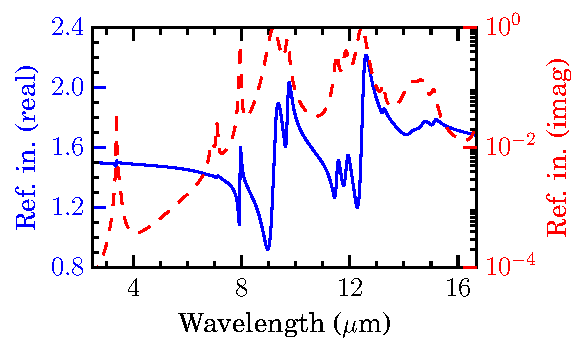
\includegraphics[width=0.8\textwidth]{./Figures/PDMS_RefractiveIndex.pdf}
\caption{\label{fig:RefInd}Real ($n$, solid line, left y-axis) and imaginary ($\kappa$, dashed line, right y-axis) parts of the complex refractive index of PDMS, respectively.}
\end{figure}

\begin{figure}
\centering
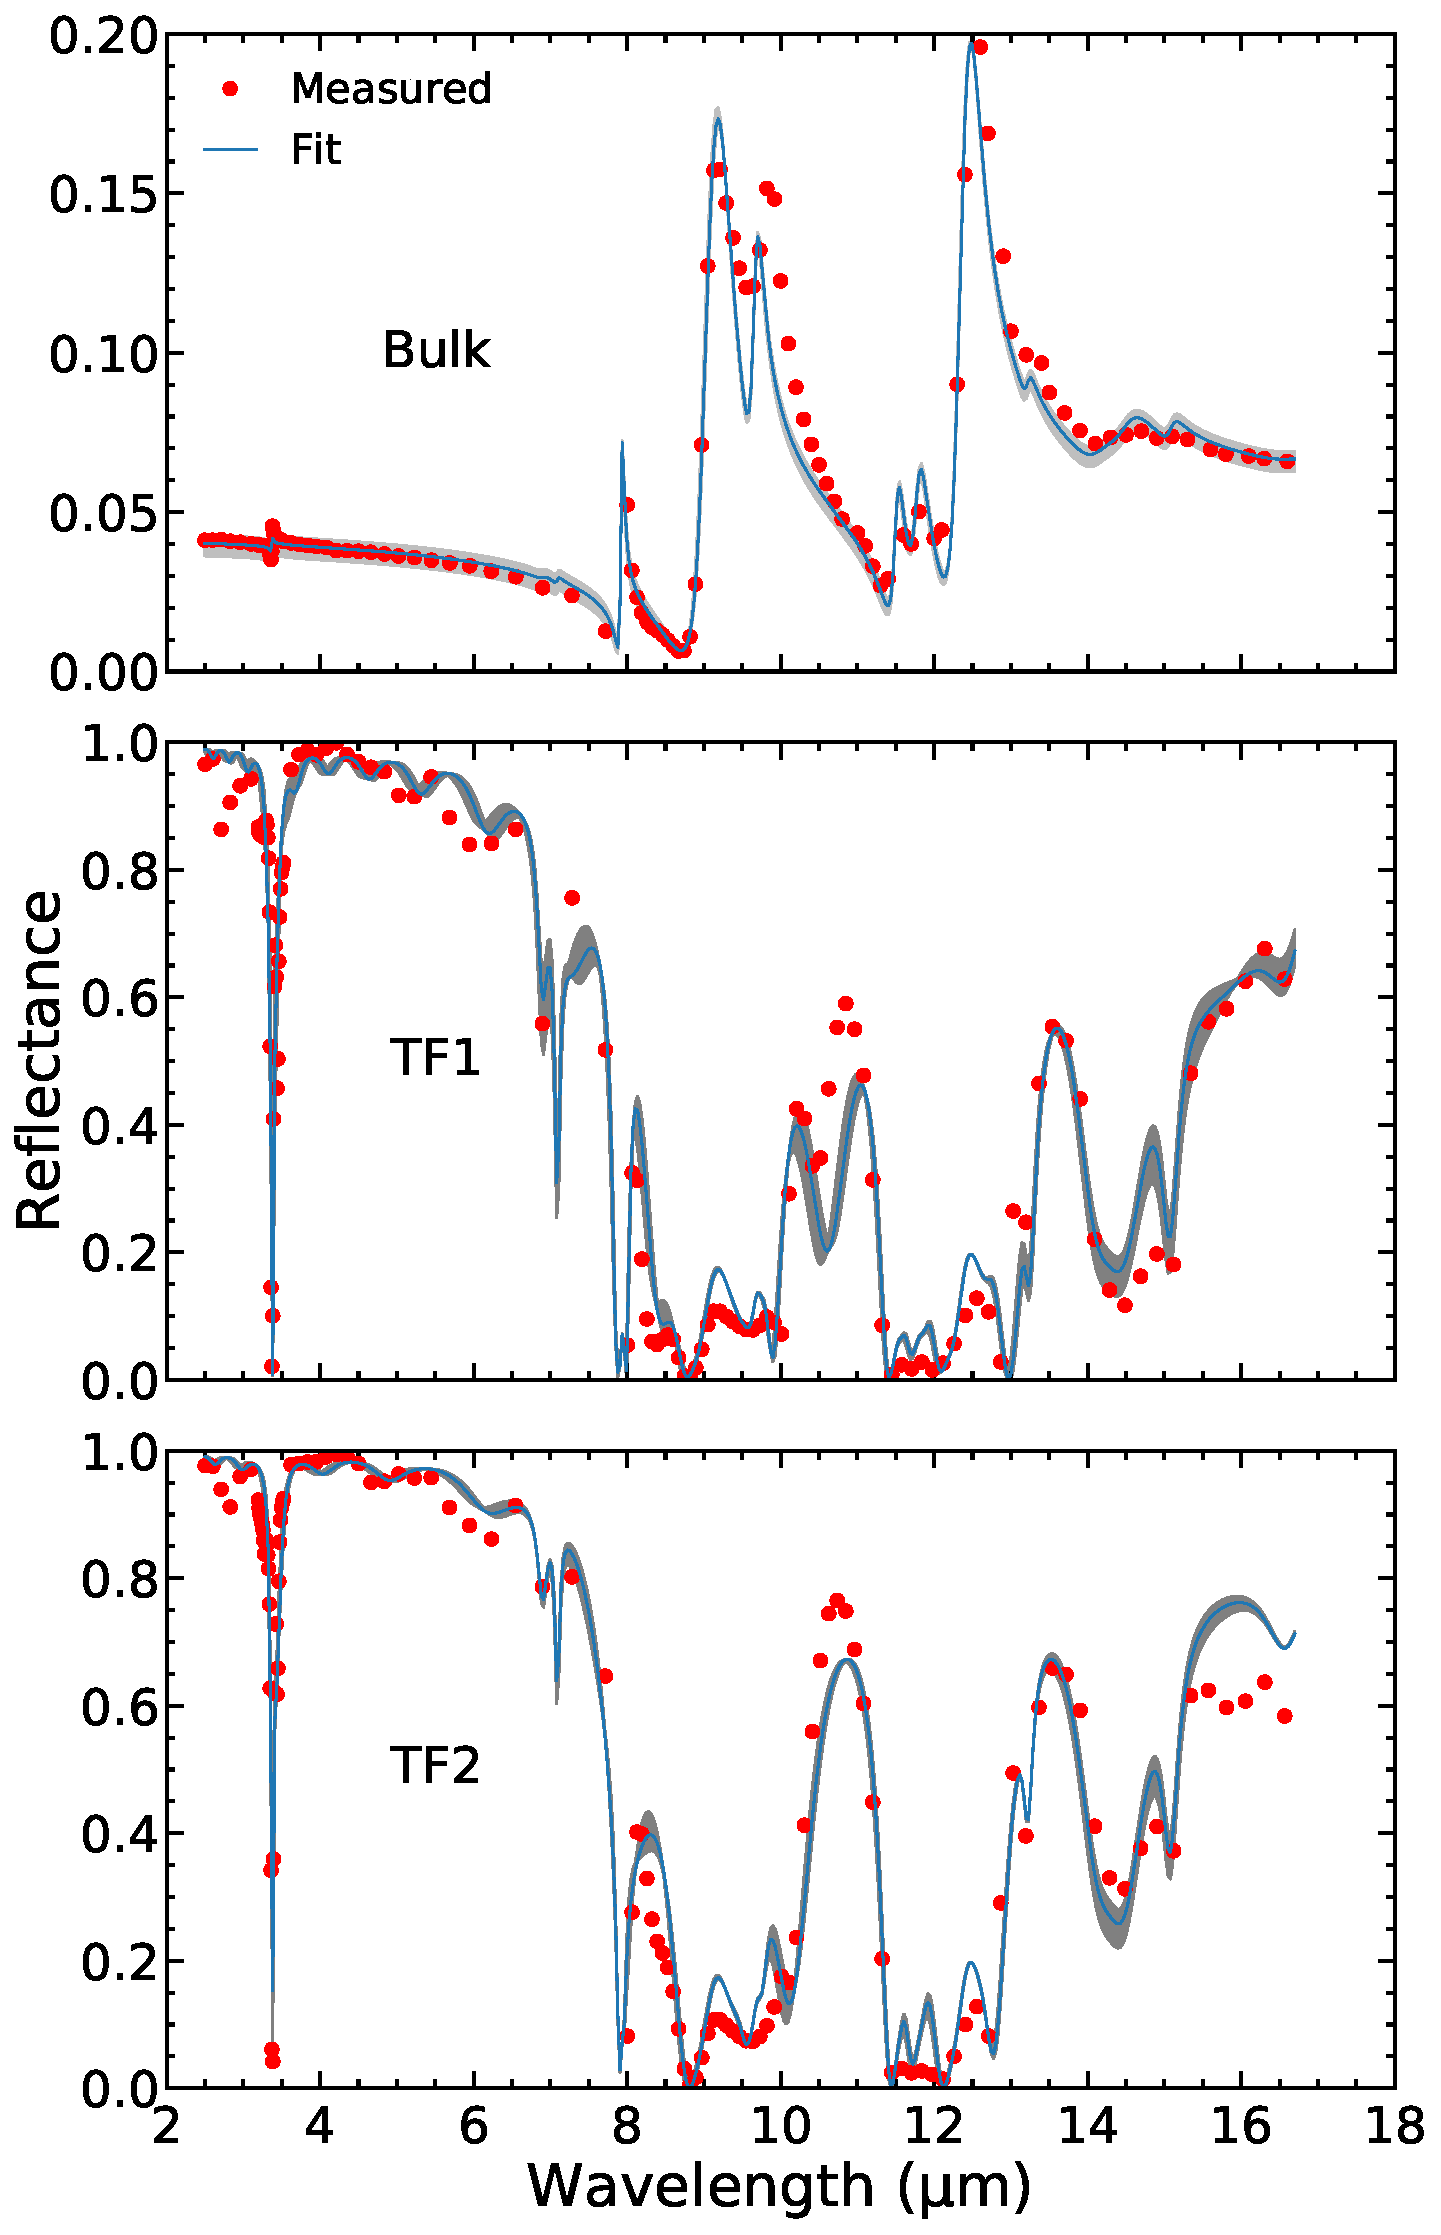
\includegraphics[width=0.75\textwidth]{./Figures/PDMS_Reflectance_and_Fit.pdf}
\caption{\label{fig:RelectanceError} Reflectance spectra of bulk and thin film PDMS samples at normal incidence obtained from FTIR reflectance measurements (circular markers); all 5000 sets of extracted oscillator parameters (gray shaded band); and the set of oscillator parameters with the lowest total error over all measurements (solid line). For clarity, only a representative number of measurement data points (circular markers) are shown.}
\end{figure}





 % Done X
\chapter[Dyadic Green's Function Formalism for Radiative Heat Transfer][Dyadic Green's Function Formalism for Radiative Heat Transfer]{Dyadic Green's Function Formalism for Radiative Heat Transfer} \label{ch:DGFs}
%
\section{Outline of Chapter}
%
In this chapter, I will describe a method outlined in Ref. \citenum{Narayanaswamy2013a} by which radiative heat transfer can determined between an arbitrary set of objects by using dyadic Green's functions. The method described is numerically exact, so long as the objects have isotropic linear optical properties and are isothermal and stationary. A key advantage of the method is that it relies on integration over the surfaces (not volumes) of the objects, which is both computationally inexpensive and analytically advantageous for composite bodies such as multilayered planes, cylinders, and spheres.

This chapter is structured as follows: in Section \ref{sec:Geometry} I will describe the geometric configuration for which the method is valid. Next, in Section \ref{sec:DGFs}, I will present dyadic Green's functions which can be used to solve for the electric and magnetic fields which mediate radiation heat transfer. Then, in Section \ref{sec:NFRHT}, I will show how the information described in the previous sections can be used to develop a Landauer-like formula for radiative energy transfer between arbitrary surfaces. The formalism will require knowledge of the Poynting vector and the fluctuation-dissipation theorem. The key component of the formalism is a transmissivity function which is defined in terms of the dyadic Green's functions of the system alone. Last, in Section \ref{sec:NFRHT_planeplane}, I will use the method developed to examine near-field radiative heat transfer between two homogeneous semi-infinite half-spaces.


\section{Geometry} \label{sec:Geometry}
%
A schematic of the system of objects that I will analyze is given in Fig. \ref{fig:DGF_Geometry}. $N$ objects are embedded in a free space region, labeled region $f$. Any object  $i$ ($1 \le i \le N$) is bound by a surface $S_{i}$ which separates object $i$ from region $f$. At every position on $S_{i}$, a unit normal vector, $\widehat{\boldsymbol{n}}_{i}$, can be defined which points outward into region $f$. Within surface $S_{i}$, object $i$ has well defined volume, temperature, and electromagnetic properties, which will be explored in great detail throughout this chapter. The free space region $f$ is itself bounded by surface $S_{E}$ (`E' subscript stands for environment). Though I specify a boundary to the free space region, the size of that boundary is allowed to grow such that region $f$ is effectively infinitely large. Region $f$ has a specified temperature and optical properties ($\varepsilon_{f}$ and $\mu_{f}$) which are dissipationless, i.e. $\varepsilon_{f}$, $\mu_{f}$ $\in \mathbb{R}$. Finally, $\boldsymbol{r}$ and $\widetilde{\boldsymbol{r}}$ represent position vectors which indicate various locations important to this work. They can be located anywhere within any object, or anywhere in region $f$.

\begin{figure}
\centering
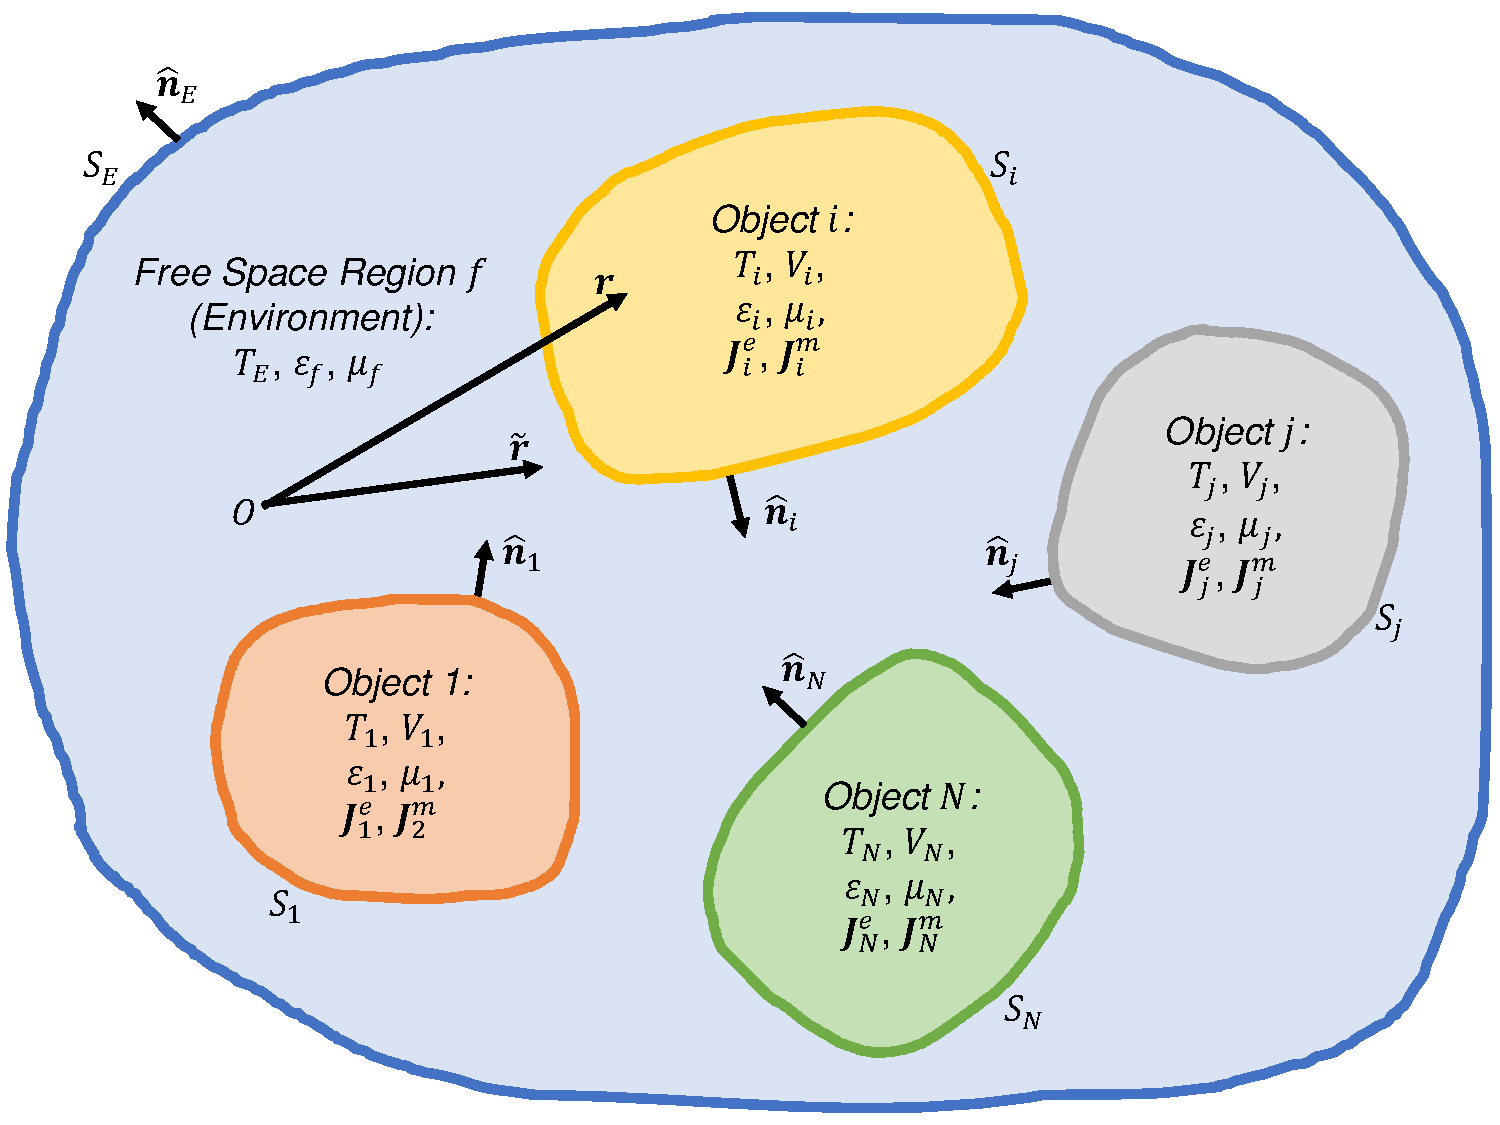
\includegraphics[width=0.8\textwidth]{./Figures/DGF_Geometry.pdf}
\caption{\label{fig:DGF_Geometry}Diagram of $N$ objects, each with its own temperature, volume, permittivity, permeability, electric free current density, and magnetic free current density. The objects are each bounded by a surface and embedded in free space region $f$, which has its own bounding surface.}
\end{figure}


\section{Dyadic Green's Functions} \label{sec:DGFs}
%
Green's functions are a powerful mathematical tool for solving boundary value problems. They represent the response of a linear differential equation at one location due to an impulse at another. A dyadic Green's function (DGF) is a Green's function which takes a vector input (for example a free current density) and produces a vector output (such as the electric field). DGFs take the form $\overline{\overline{\boldsymbol{G}}}(\boldsymbol{r}; \widetilde{\boldsymbol{r}})$ where the arguments $\boldsymbol{r}$ and $\widetilde{\boldsymbol{r}}$ are position vectors which indicate the source and response locations.

\subsection{Determining Electric and Magnetic Fields}
%
Levine and Schwinger\cite{Levine1950} first used DGFs to solve an electromagnetic boundary value problem, diffraction by an aperture in an infinite planar screen made of a conducting material. Since then, they have proven to be an invaluable tool, especially in the field of NFRHT. DGFs have been used to compute heat transfer between layered planar surfaces,\cite{Francoeur2009, Narayanaswamy2013a} spheres,\cite{Narayanaswamy2008, Sasihithlu2014, Czapla2017} and point particles,\cite{Ben-Abdallah2011, Messina2013, Asheichyk2017, Nikbakht2018} just to name a few examples.

The DGFs used to solve electromagnetism problems must satisfy the inhomogeneous vector Helmholtz equation
\begin{equation}
\boldsymbol{\nabla} \times \boldsymbol{\nabla} \times \overline{\overline{\boldsymbol{G}}}(\boldsymbol{r}; \widetilde{\boldsymbol{r}}) - k^{2}(\boldsymbol{r}) \overline{\overline{\boldsymbol{G}}}(\boldsymbol{r}; \widetilde{\boldsymbol{r}}) = \delta(\boldsymbol{r} - \widetilde{\boldsymbol{r}}) \overline{\overline{\boldsymbol{I}}}
\end{equation}

There are two variants of DGFs, electric and magnetic, which are written $\overline{\overline{\boldsymbol{G}}}_{e}(\boldsymbol{r}; \boldsymbol{\widetilde{r}})$ and $\overline{\overline{\boldsymbol{G}}}_{m}(\boldsymbol{r}; \boldsymbol{\widetilde{r}})$, respectively. The electric and magnetic variants of the DGFs can be obtained from one another by substituting $\varepsilon \leftrightarrow \mu$. Additionally, define $\overline{\overline{\boldsymbol{G}}}_{E}(\boldsymbol{r}; \boldsymbol{\widetilde{r}}) = \nabla \times \overline{\overline{\boldsymbol{G}}}_{e}(\boldsymbol{r}; \boldsymbol{\widetilde{r}})$ and $\overline{\overline{\boldsymbol{G}}}_{M}(\boldsymbol{r}; \boldsymbol{\widetilde{r}}) = \nabla \times \overline{\overline{\boldsymbol{G}}}_{m}(\boldsymbol{r}; \boldsymbol{\widetilde{r}})$, where $\nabla$ operates on functions involving $\boldsymbol{r}$ alone.

The key advantage of DGFs is that they can isolate the contributions to the electric and magnetic fields from individual sources or groups of sources, for example sources contained within a single object, like those represented in Fig. \ref{fig:DGF_Geometry}. The electric and magnetic fields themselves are superpositions of all such contributions. Define the contribution to a field $\boldsymbol{F}$ ($\boldsymbol{F}$ is $\boldsymbol{E}$ or $\boldsymbol{H}$) at location $\widetilde{\boldsymbol{r}}$ due to sources in object $i$ as $\boldsymbol{F}^{(i)}(\widetilde{\boldsymbol{r}})$. Then $\boldsymbol{F}(\widetilde{\boldsymbol{r}}) = \sum_{i=1}^{N}\boldsymbol{F}^{(i)}(\widetilde{\boldsymbol{r}})$. Obtaining $\boldsymbol{F}^{(i)}(\widetilde{\boldsymbol{r}})$ requires the inversion of Eqs. \ref{eq:MaxwellCurlElectric4} and \ref{eq:MaxwellCurlMagnetic4}. Further detail on that inversion is available in Ref. \citenum{Narayanaswamy2010}. The results of the inversion, which are presented succinctly in Ref. \citenum{Narayanaswamy2013a}, are volume integrals involving products of sources and DGFs. The volume integrals in essence calculate the net effect of all electromagnetic sources in object $i$. The volume integrals are given by
% 
\begin{subequations}
\begin{align}
\boldsymbol{E}^{(i)}(\widetilde{\boldsymbol{r}}) &= \int_{V_{i}} \left[ i \omega \mu_{0} \mu_{i} \boldsymbol{J}_{i}^{e}(\boldsymbol{r}) \cdot \overline{\overline{\boldsymbol{G}}}_{e}(\boldsymbol{r}; \widetilde{\boldsymbol{r}}) - \boldsymbol{J}_{i}^{m}(\boldsymbol{r}) \cdot \overline{\overline{\boldsymbol{G}}}_{E}(\boldsymbol{r}; \widetilde{\boldsymbol{r}}) \right] d\boldsymbol{r} \label{eq:InvertedE}
\\
\boldsymbol{H}^{(i)}(\widetilde{\boldsymbol{r}}) &= \int_{V_{i}} \left[ i \omega \varepsilon_{0} \varepsilon_{i} \boldsymbol{J}_{i}^{m}(\boldsymbol{r}) \cdot \overline{\overline{\boldsymbol{G}}}_{m}(\boldsymbol{r}; \widetilde{\boldsymbol{r}}) - \boldsymbol{J}_{i}^{e}(\boldsymbol{r}) \cdot \overline{\overline{\boldsymbol{G}}}_{M}(\boldsymbol{r}; \widetilde{\boldsymbol{r}}) \right] d\boldsymbol{r} \label{eq:InvertedH}
\end{align} \label{eq:InvertedFields}
\end{subequations}
%
where $\boldsymbol{r}$ lies within the volume of object $i$. The terms in the integrals should look familiar; they are the right hand side source terms in Eqs. \ref{eq:MaxwellCurlElectric4} and \ref{eq:MaxwellCurlMagnetic4}. 

\subsection{Boundary Conditions}
%
Solving the vector Helmholtz equation is essentially a boundary value problem, so it should come as a surprise to no one that knowledge of the boundary conditions of DGFs will prove vital. Maxwell's equations, in their integral form, guarantee continuity of the tangential components of the electric and magnetic fields across a boundary. Written in terms of DGFs, we get
%
\begin{subequations}
\begin{align}
& \widehat{\boldsymbol{n}}(\boldsymbol{r}) \times \left[\left[ \mu(\boldsymbol{r}) \overline{\overline{\boldsymbol{G}}}_{e}(\boldsymbol{r}; \widetilde{\boldsymbol{r}}) \right]\right] = 0 \\
& \widehat{\boldsymbol{n}}(\boldsymbol{r}) \times \left[\left[ \overline{\overline{\boldsymbol{G}}}_{E}(\boldsymbol{r}; \widetilde{\boldsymbol{r}}) \right]\right] = 0 \\
& \widehat{\boldsymbol{n}}(\boldsymbol{r}) \times \left[\left[ \varepsilon(\boldsymbol{r}) \overline{\overline{\boldsymbol{G}}}_{m}(\boldsymbol{r}; \widetilde{\boldsymbol{r}}) \right]\right] = 0 \\
& \widehat{\boldsymbol{n}}(\boldsymbol{r}) \times \left[\left[ \overline{\overline{\boldsymbol{G}}}_{M}(\boldsymbol{r}; \widetilde{\boldsymbol{r}}) \right]\right] = 0
\end{align} \label{eq:DGF_BCs}
\end{subequations}
%
where $\widehat{\boldsymbol{n}} \times \left[\left[ \overline{\overline{\boldsymbol{f}}} \right]\right] \equiv \widehat{\boldsymbol{n}} \times \left( \overline{\overline{\boldsymbol{f}}}_{+} - \overline{\overline{\boldsymbol{f}}}_{-} \right)$ denotes a jump condition across an interface and $\widehat{\boldsymbol{n}}$ is the unit outward normal pointing to the `+' side of the interface.\cite{Ateshian2007, Satapathy2013}


\section{Radiative Heat Transfer Between Arbitrary Surfaces} \label{sec:NFRHT}
%
Now that we are able to determine electric and magnetic fields by using the DGFs of the system, in conjunction with any sources of electromagnetic waves, we can move on to computing the net radiative transfer between objects. The strategy to compute the heat transfer using Maxwell's equations is as follows: (1) Determine the Poynting vector at the surface of an object to understand the flow of electromagnetic energy into the object. (2) Determine the time-averaged behavior of electromagnetic sources using the fluctuation-dissipation theorem. (3) Combine those results with the results of the previous section to determine formulas which give the net radiative transfer.

\subsection{Poynting Vector}
%
The Poynting vector, $\boldsymbol{P}$, is defined such that its magnitude and direction hold special significance in electromagnetism; they represent the intensity and direction of flow of electromagnetic energy at a given point. Its name is almost serendipitous, since it can be said to point in the direction of the flow. But the Poynting vector is actually named after the English physicist John Henry Poynting, who first published about it in 1884.\cite{Poynting1884}

The time-averaged contribution to the Poynting vector at a position $\widetilde{\boldsymbol{r}}$ due to sources in object $i$ given by
%
\begin{align}
\boldsymbol{P}^{(i)}(\boldsymbol{\widetilde{r}}) &= \frac{1}{2\pi} \mathrm{Re} \int_{0}^{\infty} \left< \boldsymbol{E}^{(i)}(\boldsymbol{\widetilde{r}}) \times \boldsymbol{H}^{(i)*}(\boldsymbol{\widetilde{r}}) + \boldsymbol{E}^{(i)*}(\boldsymbol{\widetilde{r}}) \times \boldsymbol{H}^{(i)}(\boldsymbol{\widetilde{r}}) \right> d\omega \label{eq:PoyntingVector}
\end{align}
%
where $\left< \cdot \right>$ denotes an ensemble average and  $\left(\cdot\right)^{*}$ is the complex conjugate. Due to linearity, the same formula is true after the substitution $\boldsymbol{P}^{(i)} \rightarrow \boldsymbol{P}$, $\boldsymbol{E}^{(i)} \rightarrow \boldsymbol{E}$, and $\boldsymbol{H}^{(i)} \rightarrow \boldsymbol{H}$. As evident by the formula, $\boldsymbol{P}^{(i)}$ is related to the cross-spectral density of the components of the electric and magnetic fields and has contributions from all frequencies. It is important to note here that, despite not being written explictly, the electric and magnetic fields both vary with frequency.

If Eqs. \ref{eq:InvertedE} and \ref{eq:InvertedH} are used to determine $\boldsymbol{E}^{(i)}(\boldsymbol{\widetilde{r}})$ and $\boldsymbol{H}^{(i)}(\boldsymbol{\widetilde{r}})$, the resulting Poynting vector gives the flow of electromagnetic energy due to sources only within the volume of object $i$. This is very useful when isolating thermal radiation between pairs of objects.

From Eq. \ref{eq:PoyntingVector}, we can see that we need to evaluate products of the electric and magnetic fields. The products contain terms which are ensemble averages of the products of the free current densities, $\boldsymbol{J}_{i}^{e}$ and $\boldsymbol{J}_{i}^{m}$. In order to evaluate those terms, we must turn to the fluctuation-dissipation theorem to better understand the statistical nature of the sources of electromagnetic radiation.


\subsection{Fluctuation-Dissipation Theorem}
%
Any object at a finite temperature, even if at equilibrium, will experience random deviations from equilibrium due to its thermal energy. When these fluctuations involve charges like electrons, the acceleration of the electrons will result in the radiation of electromagnetic waves. Although the currents due to fluctuating charges will average to zero overtime, the products of currents need not also average to zero. This is where the fluctuation-dissipation theorem comes in.

The fluctuation-dissipation theorem relates the spectral density of random fluctuations of a system to the system's dissipation. Much of the preliminary work relating fluctuation and dissipation was performed by Harry Nyquist, who investigated such a relation for conductors.\cite{Nyquist1928} His work was only applicable in the low-frequency limit. The first theory to connect fluctuations out of equilibrium and dissipation in a general linear system was completed by Callen and Welton in 1951.\cite{Callen1951} In 1953, Rytov connected thermal radiation to fluctuations currents using the fluctuation-dissipation theorem.\cite{Rytov1953, Rytov1959} His work continues to motivate modern work in NFRHT, as well as work on the van der Waals and Casimir forces.\cite{Lipshitz1956, Dzyaloshinskii1961}

The spectral densities of the components of $\boldsymbol{J}_{i}^{e}(\boldsymbol{r})$ and $\boldsymbol{J}_{i}^{m}(\boldsymbol{r})$ are related by the fluctuation-dissipation theorem of the second kind \cite{Eckhardt1982} 
%
\begin{subequations} \label{eq:FlucDiss}
\begin{align}
\left< \boldsymbol{J}_{i,p}^{e}(\boldsymbol{r}) \boldsymbol{J}_{i,q}^{e*}(\widetilde{\boldsymbol{r}}) \right> &= 2 \omega \varepsilon_{0} \mathrm{Im}{\left( \varepsilon \right)} \Theta(\omega,T) \delta \! \left( \boldsymbol{r} - \boldsymbol{\widetilde{r}} \right) \delta_{pq}
\\
\left< \boldsymbol{J}_{i,p}^{m}(\boldsymbol{r}) \boldsymbol{J}_{i,q}^{m*}(\widetilde{\boldsymbol{r}}) \right> &= 2 \omega \mu_{0} \mathrm{Im}{\left( \mu \right)} \Theta(\omega,T) \delta \! \left( \boldsymbol{r} - \boldsymbol{\widetilde{r}} \right) \delta_{pq}
\\
\left< \boldsymbol{J}_{i,p}^{e}(\boldsymbol{r}) \boldsymbol{J}_{i,q}^{m*}(\widetilde{\boldsymbol{r}}) \right> &= 0
\end{align}
\end{subequations}
%
where $p,q=1,2,3$ are the Cartesian components of the current densities, $\mathrm{Im}{\left(\cdot\right)}$ denotes the imaginary component, $T$ is the thermodynamic temperature, and $\Theta(\omega, T)$ is the average energy of a harmonic oscillator of frequency $\omega$ at temperature $T$. In Eq. \ref{eq:FlucDiss}, $\boldsymbol{J}_{i}^{e}(\boldsymbol{r})$ and $\boldsymbol{J}_{i}^{m}(\boldsymbol{r})$ represent the fluctuation and $\mathrm{Im}{\left( \varepsilon \right)}$ and $\mathrm{Im}{\left( \mu \right)}$ represent the dissipation. The delta function $\delta_{pq}$ makes clear there is no coupling between charge fluctuations in orthogonal directions. The delta function $\delta(\boldsymbol{r} - \widetilde{\boldsymbol{r}})$ shows that there is no spatial correlation in currents, and is known as the local approximation. This work will assume the validity of such an approximation, though I direct authors to Ref. \citenum{Singer2015} for work on NFRHT between non-local materials with spatial dispersion.

The average energy of a harmonic oscillator is given by
%
\begin{equation}
\begin{split}
\Theta &= k_{b} T \mathcal{X} \coth{\left( \mathcal{X} \right)}
\\
&= k_{b} T \mathcal{X} \left( 1 + \frac{2}{\exp{\left( 2 \mathcal{X} \right)} - 1} \right) 
\end{split}
\end{equation}
%
where $\mathcal{X} = \hbar\omega/(2 k_{b} T)$, $\hbar$ is the reduced Planck's constant, and $k_{b}$ is Boltzmann's constant. The lone $k_{b} T \mathcal{X}$ summand in the second line corresponds to the zero point energy. Many works in NFRHT exclude the term when defining $\Theta$ because it does not contribute to the net transfer of heat, but we keep it here for completeness.


\subsection{Heat Transfer and Conductance}
%
The goal of this chapter was to write a general formula for NFRHT in a Landauer-like form, one in which the formulas for thermal transport are given in terms of modes and probabilities of transmission of energy. Now that we can compute all the necessary terms to understand the electromagnetic fields and the flow of electromagnetic energy, we can begin to address radiative transfer. The radiative transfer through surface $S_{i}$ due to sources within object $j$ is given by
%
\begin{align}
Q_{t, j \rightarrow i} &= - \oint_{S_i} \left[ \widehat{\boldsymbol{n}}_{i}(\boldsymbol{\widetilde{r}}) \cdot \boldsymbol{P}^{(j)}(\boldsymbol{\widetilde{r}}) \right] d\boldsymbol{\widetilde{r}},
\label{eq:HeatTransfer1}
\end{align}
%
where $\boldsymbol{\widetilde{r}}$ points to positions on surface $S_{i}$ and the negative sign is required because $\widehat{\boldsymbol{n}}_{i}$ is unit outward normal of the surface and we require energy flow inward. Using Eqs. \ref{eq:PoyntingVector} (Poynting vector), \ref{eq:InvertedFields} (electric and magnetic fields), and \ref{eq:FlucDiss} (fluctuation-dissipation theorem), we can evaluate Eq. \ref{eq:HeatTransfer1} and get a result in terms of only the DGFs of the system, temperatures, and optical properties. We get
%
\begin{align}
Q_{t, j \rightarrow i} &= \frac{1}{2\pi} \int_{0}^{\infty} \left[ \Theta(\omega, T_{j}) - \Theta(\omega, T_{E}) \right] \tau_{j \rightarrow i}(\omega) d\omega
\label{eq:HeatTransfer2}
\end{align}
%
where $\tau_{j \rightarrow i}(\omega)$ is a temperature-independent transmissivity function for energy transfer between objects $i$ and $j$. In some sense, it is a catch-all function for all the terms you get when you evaluate Eq. \ref{eq:HeatTransfer1}. But the function has a number of convenient features which will be discussed at length in the next subsection. The net radiative transfer from object $j$ to object $i$ is given by
%
\begin{equation}
\begin{split}
Q_{t, j \rightarrow i}^{(\mathrm{net})} &= Q_{t, j \rightarrow i} - Q_{t, i \rightarrow j} = \int_{0}^{\infty} Q_{j \rightarrow i}^{(\mathrm{net})}(\omega) d\omega
\\
&= \frac{1}{2\pi} \int_{0}^{\infty} \left[ \Theta(\omega, T_{j}) - \Theta(\omega, T_{i}) \right] \tau_{j \rightarrow i}(\omega) d\omega
\label{eq:NetHeatTransfer}
\end{split}
\end{equation}

This simplification is enabled because $\tau_{i \rightarrow j} = \tau_{j \rightarrow i}$.\cite{Narayanaswamy2013a} From Eq. \ref{eq:NetHeatTransfer}, is it clear to see $Q_{t,j \rightarrow i}^{(\mathrm{net})} = - Q_{t,i \rightarrow j}^{(\mathrm{net})}$, which fits with our expectation for radiative transfer.

An additional quantity useful to analyzing systems of objects exchanging radiation is the conductance. Conductance is the proportionality constant between $Q$ and $\Delta T$, and can be used to linearize the temperature dependence of thermal radiation when $\Delta T$ is small. Define two conductances, a spectral ($G$) and a total conductance ($G_{t}$), given by
%
\begin{align}
G_{j \rightarrow i}(\omega, T) &= \lim_{T_{j},T_{i} \rightarrow T} \frac{Q_{j \rightarrow i}^{\mathrm{(net)}}(\omega)}{T_{j}-T_{i}} =  \frac{\partial \Theta}{\partial T} \tau_{j \rightarrow i} \left( \omega \right)
\\
G_{t, j \rightarrow i}(T) &= \frac{1}{2\pi} \int_{0}^{\infty} G_{j \rightarrow i}(\omega, T) d\omega
\end{align}

Working with conductance has the advantage of reducing the number of temperatures variables to one. To calculate conductances, the temperature dependence is captured by the temperature derivative of $\Theta$
%
\begin{equation} \label{eq:TemperatureDerivative}
\begin{split}
\frac{\partial \Theta}{\partial T} &= k_{b} \mathcal{X}^{2} \csch^{2}{\left( \mathcal{X} \right)}
\\
&= k_{b} \left( 2 \mathcal{X} \right)^{2} \frac{ \exp{\left( 2 \mathcal{X} \right)} }{ \left( \exp{\left( 2 \mathcal{X} \right)} - 1 \right)^{2} }
\end{split}
\end{equation}

Spectral conductance is often expressed in different units in different papers, but changes of variable can be performed to transform between units. A definition of spectral conductance is valid so long as the integral defintion of total conductance computes to the same value, regardless of the units used. For example, in Fig. \ref{fig:ThreeSpheres_SCUFFEM} I present $\tau_{j \rightarrow i}(\lambda)$ in units of \si{\per\second \per\micro\meter}, where $\lambda = 2 \pi c / \omega$ is the vacuum wavelength and $c$ is speed of light in vacuum. This version of spectral conductance is obtained from $\tau_{j \rightarrow i}(\lambda) = c \lambda^{-2} \tau_{j \rightarrow i}(\omega)$ and the corresponding integral definition for total conductance is
%
\begin{equation} \label{eq:TotalConductance_wavelength}
\begin{split}
G_{t,j \rightarrow i}(T) &= \int_{0}^{\infty} G_{j \rightarrow i}(\lambda, T) d\lambda
\\
&= \int_{0}^{\infty} k_{b} \mathcal{X}^{2} \csch^{2}{\left( \mathcal{X} \right)} \tau_{j \rightarrow i}(\lambda) d\lambda 
\end{split}
\end{equation}


\subsection{Transmissivity Function}
%
As was stated earlier, DGFs take the form $\overline{\overline{\boldsymbol{G}}}(\boldsymbol{r}; \widetilde{\boldsymbol{r}})$ where the arguments $\boldsymbol{r}$ and $\widetilde{\boldsymbol{r}}$ are position vectors which indicate the source and response locations. Depending on which regions $\boldsymbol{r}$ and $\widetilde{\boldsymbol{r}}$ are located, both the DGFs themselves and the form of the transmissivity function must change. The transmissivity function was derived using Eq. \ref{eq:InvertedFields} (volume integration) and Eq. \ref{eq:HeatTransfer1} (surface integration). That asymmetry has a number of disadvantages, primarily that it obscures the symmetry of radiative heat transfer. Since emission and absorption of electromagnetic waves are volumetric phenomena, it might seem intuitive to expect the expression for the transmissivity function for energy transfer to contain two volume integrals, and thus to convert the surface integral to a volume integral. Double volume integral was the approach that allowed Polder and van Hove to derive their plane-plane NFRHT\cite{Polder1971} and for Narayanaswamy and Chen to derive the first sphere-sphere NFRHT result.\cite{Narayanaswamy2008} But that approach is limited because any composite bodies would require volume integration over each interior region separately. While that is not impossible, it is cumbersome.

If the volumes are isothermal, the properties of the vector Helmholtz equation allow us to convert volume integrals into surface integrals. If the volume integral is converted to a surface integral, we get the approach called the ``interior method'' by Narayanaswamy and Zheng in Ref. \citenum{Narayanaswamy2013a}. When using the interior method, though the integrations occur on the two surfaces, $\boldsymbol{r}$ and $\widetilde{\boldsymbol{r}}$ must approach the two surfaces from the insides of the objects. The transmissivity function for such a situation is given by
%
\begin{align}
\tau_{j \rightarrow i} (\omega) &= 2 \mathrm{Re} \mathrm{Tr} \oint_{S_i} d\boldsymbol{r} \oint_{S_j} d\boldsymbol{\widetilde{r}}
\left[ \!\! \begin{array}{r} \! \! \left( \frac{\omega}{c} \right)^{2} \! \! \varepsilon^{*}(\boldsymbol{r}) \mu(\boldsymbol{r}) \bigg[ \boldsymbol{\widehat{n}}_{i}(\boldsymbol{r}) \times \overline{\overline{\boldsymbol{G}}}_{e}(\boldsymbol{r}, \widetilde{\boldsymbol{r}}) \bigg] \! \cdot \! \bigg[ \boldsymbol{\widehat{n}}_{j}(\boldsymbol{\widetilde{r}}) \times \overline{\overline{\boldsymbol{G}}}_{m}^{T}(\boldsymbol{r}, \boldsymbol{\widetilde{r}}) \bigg]^{*} \\
+ \bigg[ \boldsymbol{\widehat{n}}_{i}(\boldsymbol{r}) \times \overline{\overline{\boldsymbol{G}}}_{M}(\boldsymbol{r}, \boldsymbol{\widetilde{r}}) \bigg] \! \cdot \! \bigg[ \boldsymbol{\widehat{n}}_{j}(\boldsymbol{\widetilde{r}}) \times \overline{\overline{\boldsymbol{G}}}_{E}^{T}(\boldsymbol{r}, \boldsymbol{\widetilde{r}}) \bigg]^{*}
\end{array} \!\! \right] \label{eq:Transmissivity_Interior}
\end{align}

In some ways, the double surface integral formula for the transmissivity function appears similar to the formula for a view factor \cite{Howell2011} in classical radiative transfer. The view factor, however, is a purely geometric property of just two objects, irrespective of any other objects present, whereas the DGFs contained within the transmissivity function automatically account for the effects of all objects present. Furthermore classical approaches such as thermal circuits or Gebhart factors \cite{Gebhart1961}, when using view factors in their calculations, assume objects emit diffusly with well-defined emissivities. DGF approaches, and therefore the transmissivity function, are exact in all situations where Maxwell's equations are valid, which includes objects with super-Planckian (greater than that of a blackbody) effective emissivities.

The boundary conditions given by Eq. \ref{eq:DGF_BCs} allow us to move from the interior method to an ``exterior method," one for which $\boldsymbol{r}$ and $\widetilde{\boldsymbol{r}}$ must approach the two surfaces from the outsides of the objects, in free-space region $f$. The advantage of this approach is that the same formalism can be used for homogeneous or composite objects. The transmissivity function for that case is given by
%
\begin{align}
\tau_{j \rightarrow i} (\omega) &= 2 \mathrm{Re} \mathrm{Tr} \oint_{S_i} d\boldsymbol{r} \oint_{S_j} d\boldsymbol{\widetilde{r}}
\left[ \begin{array}{r} k_{f}^{2} \bigg[ \boldsymbol{\widehat{n}}_{i}(\boldsymbol{r}) \times \overline{\overline{\boldsymbol{G}}}_{e}(\boldsymbol{r}, \widetilde{\boldsymbol{r}}) \bigg] \cdot \bigg[ \boldsymbol{\widehat{n}}_{j}(\boldsymbol{\widetilde{r}}) \times \overline{\overline{\boldsymbol{G}}}_{m}^{T}(\boldsymbol{r}, \boldsymbol{\widetilde{r}}) \bigg]^{*} \\
+ \bigg[ \boldsymbol{\widehat{n}}_{i}(\boldsymbol{r}) \times \overline{\overline{\boldsymbol{G}}}_{M}(\boldsymbol{r}, \boldsymbol{\widetilde{r}}) \bigg] \cdot \bigg[ \boldsymbol{\widehat{n}}_{j}(\boldsymbol{\widetilde{r}}) \times \overline{\overline{\boldsymbol{G}}}_{E}^{T}(\boldsymbol{r}, \boldsymbol{\widetilde{r}}) \bigg]^{*}
\end{array} \right] \label{eq:Transmissivity_Exterior}
\end{align}

At first glance, the transmissivity function for the exterior method does not appear very different than that of the interior method. The key difference between the two is that the DGFs needed to use this formalism are different than those for the interior method. The DGFs must be determined such that both of the position vector arguments are located in free space region $f$, just outside the surfaces of objects $i$ and $j$. The exterior method will be the approach favored throughout this work.


\section{Radiative Heat Transfer Between Planar Bodies} \label{sec:NFRHT_planeplane}
%
The NFRHT between two planar half-spaces has been well-studied since Polder and van Hove first published their work in 1971.\cite{Polder1971} In this section, I will present theoretical and numerical results for plane-plane NFRHT. Using the exterior method (see Ref. \citenum{Narayanaswamy2013a} for the appropriate DGFs), the transmissivity (per unit area) between two semi-infinite half-spaces is given by 
%
\begin{equation}
\frac{\tau_{1 \rightarrow 2}(\omega)}{A} = \frac{1}{2\pi} \int_{0}^{\infty} \left[ \mathcal{T}^{(s)}(k_{\rho}) + \mathcal{T}^{(p)}(k_{\rho}) \right] k_{\rho} dk_{\rho}
\end{equation}
%
where
\begin{equation}
\mathcal{T}^{(\alpha)}(k_{\rho}) = \left\{ \begin{array}{lcc}
\frac{\left( 1 - \left| \widetilde{r}_{1}^{(\alpha)} \right|^{2} \right) \left( 1 - \left| \widetilde{r}_{2}^{(\alpha)} \right|^{2} \right)}{\left| 1 - \widetilde{r}_{1}^{(\alpha)} \widetilde{r}_{2}^{(\alpha)} \exp{\left( 2ik_{z,0} l \right)} \right|^{2}} & \mathrm{if} & 0 \le k_{\rho} \le \omega/c \\
\frac{4 \mathrm{Im}\left( \widetilde{r}_{1}^{(\alpha)} \right) \mathrm{Im}\left( \widetilde{r}_{2}^{(\alpha)} \right) \exp{\left( 2ik_{z,0} l \right)}}{\left| 1 - \widetilde{r}_{1}^{(\alpha)} \widetilde{r}_{2}^{(\alpha)} \exp{\left( 2ik_{z,0} l \right)} \right|^{2}} & \mathrm{if} & \omega/c < k_{\rho}
\end{array} \right.
\end{equation}
%

Here, $k_{\rho}$ is the in-plane component of the wavevector, $k_{z}$ is the component of the wavevector normal to the surface, $l$ is the separation distance between the two half-spaces, $\widetilde{r}^{(\alpha)}$ is the effective Fresnel coefficient, and $\alpha$ is either the $s$ or $p$ polarization. Information on computing the Fresnel reflection coefficients is found in Appendix \ref{ap:FresnelCoefficients}.

The transmissivity function between two planar media has a piecewise definition, dependent on the value of $k_{\rho}$. For $0 \le k_{\rho} \le \omega/c$, radiation is exchanged by propagating waves. These are the waves accounted for by CRT. For $\omega/c < k_{\rho}$, evanescent waves are responsible for radiative transfer. Evanescent waves are surface waves that exponentially decrease in magnitude as the distance from the surface increases. Evanescent waves are the result of total internal reflection and they are not able to contribute to radiative transfer from a half-space to free space so they do not show up in emissivity calculations. If a second object comes into close proximity to an object with evanescent surface waves and the evanescent wave intersects the second object, then energy may be transferred. This is referred to as frustrated total internal reflection by the optics community and often called photon tunneling in the NFRHT community due to the analogous math to quantum mechanical tunneling.\cite{Zhu1986}

Evanescent waves are essentially the secret sauce of NFRHT; they enable super-Planckian radiative transfer by serving as a second channel to transfer heat. The most important types of evanescent waves to NFRHT are those which couple to phonons (lattice vibrations) within an object to form a resonant quasiparticle called a surface phonon polariton (SPhP).\cite{Mirlin1982} This coupling can only occur for the $p$ polarization when $\mathrm{Re}(\varepsilon) < -1$ and $\mathrm{Im}(\varepsilon) \ll 1$.\cite{Petersen2013}


\subsection{Numerical Results}
%
Numerical results for NFRHT between two half-spaces composed of polar dielectrics (silicon dioxide and silicon carbide), polymer dielectrics (PDMS and PMMA), and metals (gold and silver) are presented in Figs. \ref{fig:PlanePlane_total} and \ref{fig:PlanePlane_spectral_onegap}. All conductances are computed at $T = 300$ \si{\kelvin} and are normalized by the conductance between two blackbodies. The spectral conductance between two blackbodies is given by
%
\begin{align} \label{eq:SpecCond_BB}
G_{j \rightarrow i,BB}(\lambda, T) &= \left[ \frac{ \left( \frac{8 \pi^{3} c^{3} \hbar^{2}}{k_{b} T^{2} \lambda^{6}} \right) \exp{\left( \frac{2 \pi \hbar c}{k_{b} T \lambda} \right)} }{ \left[ \exp{\left( \frac{2 \pi \hbar c}{k_{b} T \lambda} \right)} - 1 \right]^{2} } \right] A_{j} F_{j \rightarrow i},
\end{align}
%
and the total conductance is given by
%
\begin{align} \label{eq:TotalCond_BB}
G_{t,j \rightarrow i,BB}(T) &= \int_{0}^{\infty} G_{j \rightarrow i,BB}(\lambda, T) d\lambda = 4 \sigma T^{3} A_{j} F_{j \rightarrow i},
\end{align}
%
where $A_{j}$ is the surface area of object $j$, $F_{j \rightarrow i}$ is the radiative view factor from object $j$ to object $i$, and $\sigma=\pi^{2} k_{b}^{4}/60c^{2}\hbar^{3}$ is the Stefan-Boltzmann constant. See Appendix \ref{ap:CRT} for further details.

Figure \ref{fig:PlanePlane_spectral_onegap} shows the total conductance as a function of distance. In the near-field ($D < 10$ \si{\micro\meter}), all materials deviate from the constant behavior predicted by CRT and begin to show higher heat transfer rates. The dielectric materials achieve a slope of $\sim D^{-2}$, which is a telltale sign of evanescent wave domination over NFRHT for planar media. Polar materials, which support SPhP modes, show higher heat transfer than polymers, which themselves outperform metals at almost all gaps. Metals tend to level out in the extreme near-field, which indicates that high k-modes do not contribute as heavily to heat transfer between metals as between dielectrics.

\begin{figure}
\centering
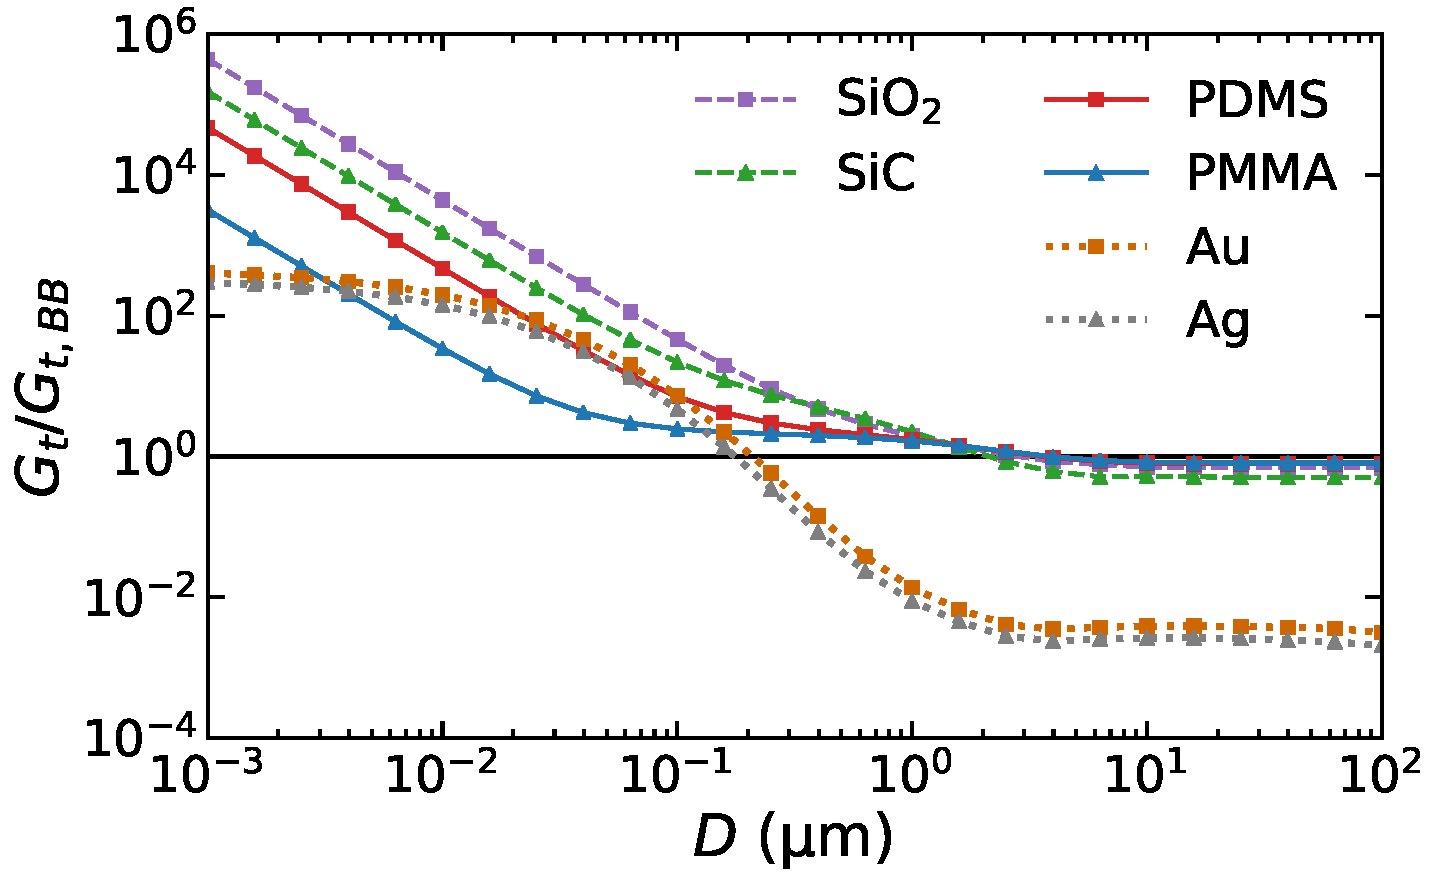
\includegraphics[width=0.8\textwidth]{./Figures/NFRHT_planeplane_total.pdf}
\caption{\label{fig:PlanePlane_total}Total conductance between two semi-infinite planar bodies. The conductance is computed for polar dielectrics (SiO$_{2}$ and SiC), polymers (PDMS and PMMA), and metals (Au and Ag). The conductance is normalized in the plot by that of two blackbodies ($G_{t,BB}/A = 6.12$ \si{\watt\per\square\meter\per\kelvin} where $A$ is the surface area). The solid black line lies at an ordinate of 1 (blackbody behavior) for all values of abscissa.}
\end{figure}

Figure \ref{fig:PlanePlane_total} shows the spectral conductance at a fixed separation distance of 0.1 \si{\micro\meter}. This distance was chosen because it lies safely within the near-field.  Dielectric materials show mostly level behavior (indicating a graybody approximation is valid at those wavelengths), with some peaks seemingly superimposed on top. The peaks correspond to the locations of resonances of the dielectric function of each material.\cite{Spitzer1959, Srinivasan2016, Tsuda2018} The three largest peaks present (two large peaks for silicon dioxide at 8.5 \si{\micro\meter} and 20 \si{\micro\meter} and one large peak at 10.5 \si{\micro\meter} for silicon carbide) correspond to SPhP modes. The other peaks occur due to optical resonances that do not qualify as SPhP modes. Those peaks, such as the numerous peaks in the spectra of PDMS and PMMA, tend to be much smaller. Unsurprisingly, the metals act unlike any other material and do not conform to the shape of a blackbody distribution.

\begin{figure}
\centering
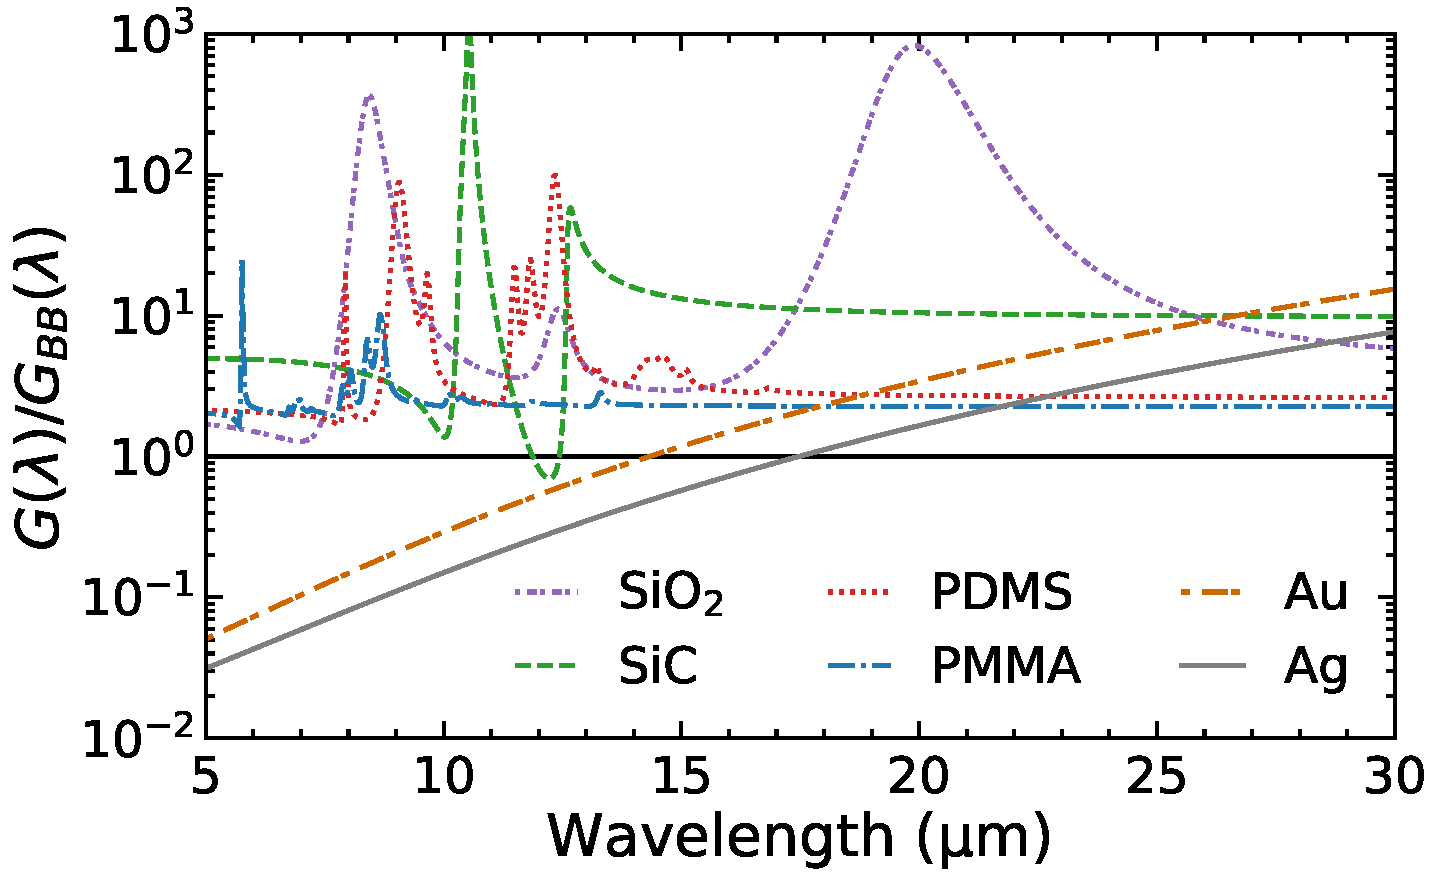
\includegraphics[width=0.8\textwidth]{./Figures/NFRHT_planeplane_spectral_fixedgap.pdf}
\caption{\label{fig:PlanePlane_spectral_onegap}Spectral conductance between two semi-infinite planar bodies with a separation distance of 0.1 \si{\micro\meter}. The conductance is computed for polar dielectrics (SiO$_{2}$ and SiC), polymers (PDMS and PMMA), and metals (Au and Ag). The conductance is normalized in the plot by that of two blackbodies. The solid black line lies at an ordinate of 1 (blackbody behavior) for all values of abscissa.}
\end{figure}

Reviewing NFRHT between planar surfaces was meant to demonstrate some of the common features of NFRHT in the simplest test-case. Many of these characteristics will appear again when examining NFRHT between spheres. The details of that configuration are presented in Chapters \ref{ch:model} and \ref{ch:results}. % Done X
\chapter[Model for Near-Field Radiative Heat Transfer Between Spherical Bodies][Model for Near-Field Radiative Heat Transfer Between Spherical Bodies]{Model for Near-Field Radiative Heat Transfer Between Spherical Bodies} \label{ch:model} \allowdisplaybreaks

\begin{quote}
    We choose to work with spheres not because they are easy, but because they are hard; because that goal will serve to organize and measure the best of our energies and skills, because that challenge is one that we are willing to accept, one we are unwilling to postpone, and one we intend to win, and the others, too. \sourceatright{John F. Kennedy, probably}
\end{quote}

\section{Introduction}
%
In this chapter, we will develop a model for NFRHT between spherical objects, and between a spherical object and its environment. Specifically, we will examine the case of a linear chain of spheres, a chain in which the centers of every sphere lie on a common axis. I published this work in Refs. \citenum{Czapla2017} and \citenum{Czapla2018}. Spheres are an important geometry to investigate because of their numerous useful properties: they are compact objects with a convenient coordinate system, they have rotational symmetry, in the limit as one sphere is much larger than the second you recover a sphere-plane geometry, small spheres can approximate dipoles, etc. For these reasons and more, a model of NFRHT involving spheres is an attractive tool to add to the the toolbox of the NFRHT community.

I will proceed as follows: first, I will provide the geometrical definitions required to describe a linear chain of spheres. Next, I will mathematically define vector spherical waves and demonstrate how to translate them between coordinate systems. After that, I will use the vector spherical waves to construct the DGFs of the system. Finally, I will use the DGFs to solve for the transmissivity which describes sphere-sphere and sphere-environment NFRHT.

\section{Geometry of Linear Chain}
%
The configuration of the chain of spheres is shown in Fig. \ref{fig:Chain_Geometry}. In Fig. \ref{fig:Chain_Geometry}A, an individual sphere, labeled sphere $i$, is depicted. Sphere $i$ has an outer radius, $\rho_{i}$. Internally, it may be homogeneous or composed of spherically symmetric layers. Coordinate system $i$ is fixed to the center of sphere $i$. Any position vector, $\boldsymbol{r}$ or $\widetilde{\boldsymbol{r}}$, when written in coordinate system $i$, is denoted $\boldsymbol{r}_{i}$ or $\widetilde{\boldsymbol{r}}_{i}$, respectively. 

Figure \ref{fig:Chain_Geometry}B depicts a section of a linear chain of $N_{s}$ spheres, which is embedded in free space (referred to as region $f$). The $z$-axis of coordinate system $i$ ($1 \le i \le N_{s}$) is aligned down the central axis of the chain. The $x$-axes of all coordinate systems are parallel, and similarly so are the $y$-axes.

The spheres are numbered $1$ through $N_{s}$, such that their labels increase along the positive $z$-direction (of any coordinate system). Any two spheres, $i$ and $j$, are separated by center-to-center distance $d_{i,j}$ and the minimum separation between them is $D_{i,j} = | d_{i,j} | - \rho_{i} - \rho_{j}$ (not depicted explicitly in Fig. \ref{fig:Chain_Geometry}). The sign of $d_{i,j}$ is positive if $j > i$ and negative if $j < i$.

\begin{figure}
\centering
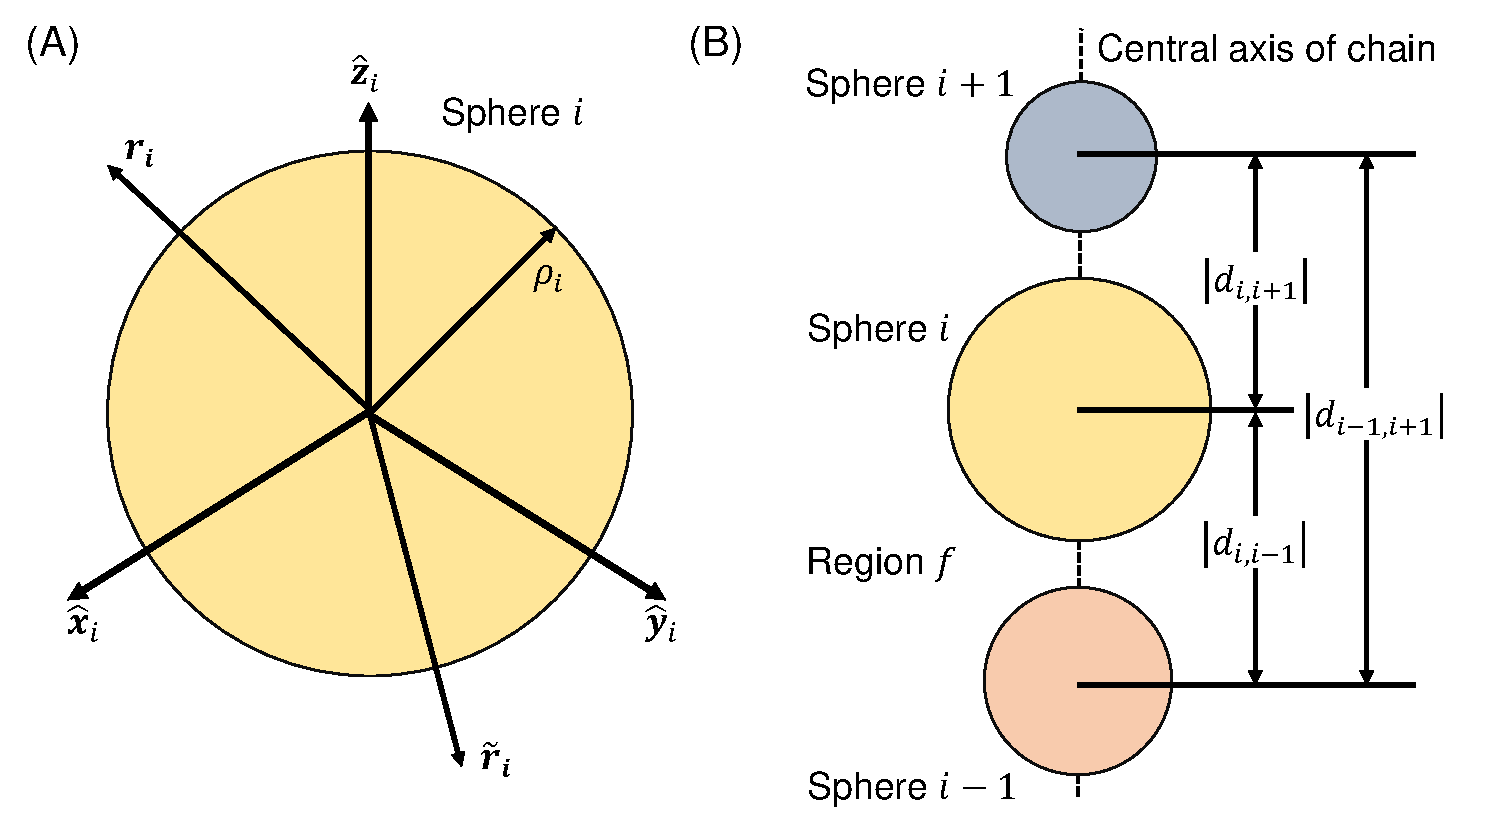
\includegraphics[width=0.8\textwidth]{./Figures/Chain_Geometry.pdf}
\caption{\label{fig:Chain_Geometry}Configuration of spheres in chain. (A) Single sphere $i$ and its associated coordinate system. (B) Section from a linear chain of spheres embedded in region $f$.}
\end{figure}


\section{Spherical Waves}

\subsection{Spherical Coordinate System}
Throughout this chapter, we will be working extensively in spherical coordinates. The convention used to define unit vectors in spherical coordinates varies by field, so a depiction of the convention used henceforth is given as Fig. \ref{fig:SphericalCoordinates}. In our system, $\phi$ defines the azimuthal direction and $\theta$ defines the polar (zenith) angle. The radial distance from the origin is given by $r$.
%
\begin{figure}
\centering
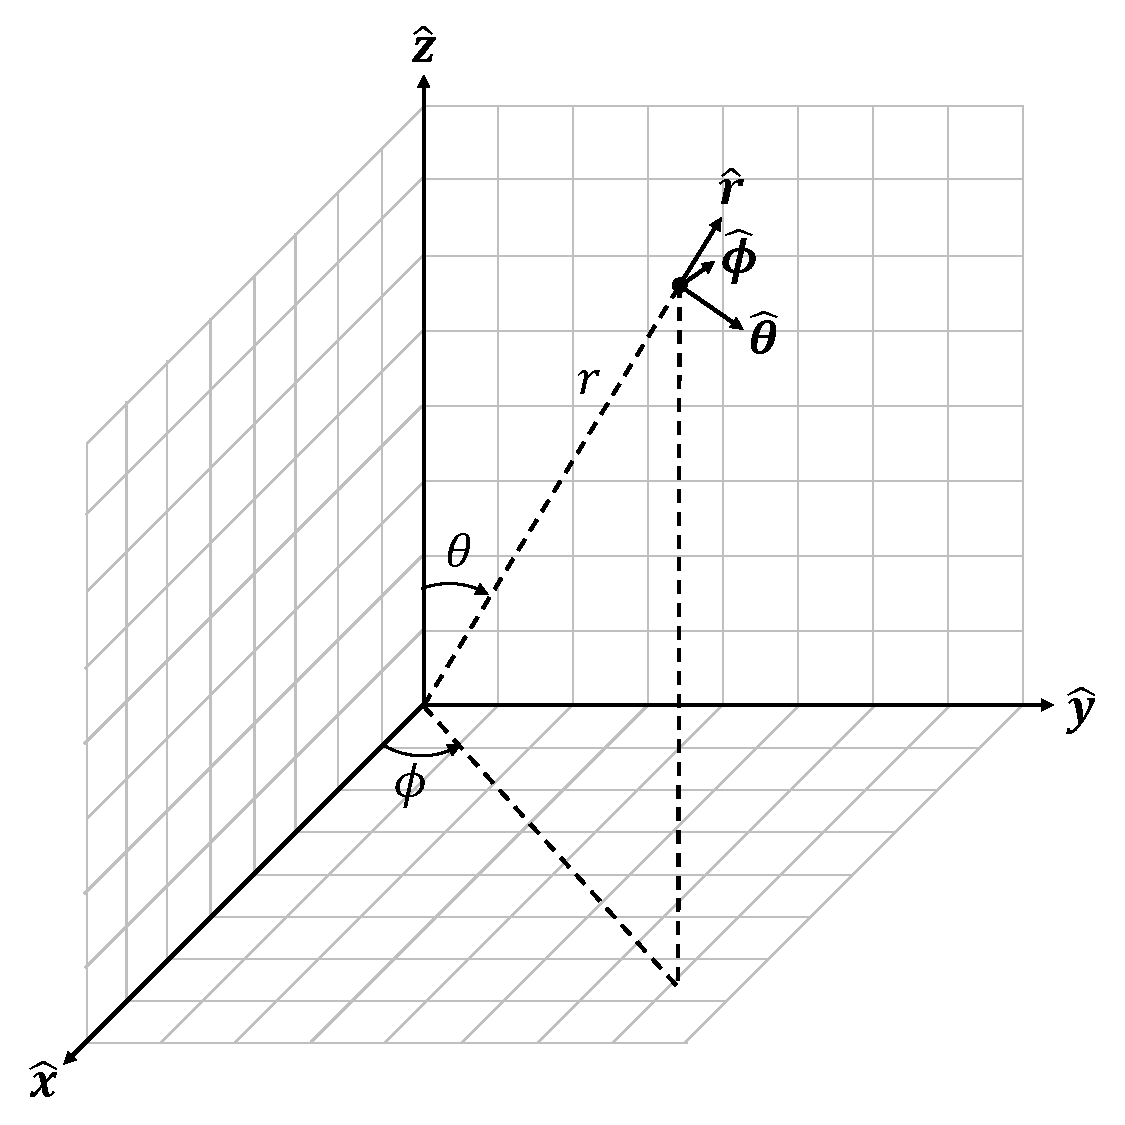
\includegraphics[width=0.8\textwidth]{./Figures/SphericalCoordinates.pdf}
\caption{\label{fig:SphericalCoordinates}Spherical coordinate system convention used in this work.}
\end{figure}

\subsection{Vector Eigenfunctions}
%
When expressed in a spherical coordinate system, the solutions to the homogeneous vector Helmholtz equation are vector spherical waves (VSWs). Three such VSWs exist: $\boldsymbol{L}_{lm}^{(p)}(k\boldsymbol{r})$, $\boldsymbol{M}_{lm}^{(p)}(k\boldsymbol{r})$, and $\boldsymbol{N}_{lm}^{(p)}(k\boldsymbol{r})$. The value of $p$ gives the radial behavior (to be discussed shortly) and $(l,m)$ gives the order of a VSW. The divergence of $\boldsymbol{M}_{lm}^{(p)}(k\boldsymbol{r})$ and $\boldsymbol{N}_{lm}^{(p)}(k\boldsymbol{r})$ is zero, while the curl of $\boldsymbol{L}_{lm}^{(p)}(k\boldsymbol{r})$ is zero. Because Maxwell's equations require divergence-free fields at source-free locations (see Eqs. \ref{eq:ElectricDivergence} and \ref{eq:MagneticDivergence}), only $\boldsymbol{M}_{lm}^{(p)}(k\boldsymbol{r})$ and $\boldsymbol{N}_{lm}^{(p)}(k\boldsymbol{r})$ are required to express the electric and magnetic fields in the eigenfunction expansions in this work.

The requisite VSWs are defined as
%
\begin{align}
\boldsymbol{M}_{l m}^{(p)}(k \boldsymbol{r}) = & z_{l}^{(p)}(kr) \boldsymbol{V}_{lm}^{(2)}(\theta, \phi),
\\
\boldsymbol{N}_{l m}^{(p)}(k \boldsymbol{r}) = & \zeta_{l}^{(p)}(kr) \boldsymbol{V}_{lm}^{(3)}(\theta, \phi) + \frac{\sqrt{l(l+1)}}{kr} z_{l}^{(p)}(kr) \boldsymbol{V}_{lm}^{(1)}(\theta, \phi),
\end{align}
%
where $r = |\boldsymbol{r}|$, $z_{l}^{(p)}(kr)$ is the spherical Bessel ($p=1$) or spherical Hankel ($p=3$) function of the first kind and $ \zeta_{l}^{(p)}(kr) = \frac{1}{kr}\frac{d}{d(kr)} ( kr z_{l}^{(p)}(kr) )$.  $\boldsymbol{V}_{lm}^{(1)}(\theta, \phi)$, $\boldsymbol{V}_{lm}^{(2)}(\theta, \phi)$, and $\boldsymbol{V}_{lm}^{(3)}(\theta, \phi)$ are the vector spherical harmonics of order $(l,m)$ for polar and azimuthal angles $\theta$ and $\phi$, respectively. They are defined as
%
\begin{align}
\boldsymbol{V}_{lm}^{(1)}(\theta, \phi) &= Y_{lm}(\theta, \phi) \boldsymbol{\widehat{r}},
\\
\boldsymbol{V}_{lm}^{(2)}(\theta, \phi) &= \frac{r}{\sqrt{l(l+1)}} \boldsymbol{\nabla} Y_{lm}(\theta, \phi) \times \boldsymbol{\widehat{r}},
\\
%&= \frac{1}{\sqrt{l(l+1)}} \left( \frac{im}{\sin{\theta}}Y_{lm}(\theta, \phi) \boldsymbol{\widehat{\theta}} - \frac{\partial}{\partial \theta} Y_{lm}(\theta, \phi) \boldsymbol{\widehat{\phi}} \right)
%\\
\boldsymbol{V}_{lm}^{(3)}(\theta, \phi) &= \frac{r}{\sqrt{l(l+1)}} \boldsymbol{\nabla} Y_{lm}(\theta, \phi),
%\\
%&= \frac{1}{\sqrt{l(l+1)}} \left( \frac{\partial}{\partial \theta} Y_{lm}(\theta, \phi) \boldsymbol{\widehat{\theta}} + \frac{im}{\sin{\theta}}Y_{lm}(\theta, \phi) \boldsymbol{\widehat{\phi}} \right)
\end{align}
%
where $Y_{lm}(\theta, \phi)$ is the scalar spherical harmonic of order $(l,m)$ and $\boldsymbol{\widehat{r}}$, $\boldsymbol{\widehat{\theta}}$, and $\boldsymbol{\widehat{\phi}}$ are the unit vectors of the spherical coordinate system (see Fig. \ref{fig:SphericalCoordinates}). Scalar spherical harmonics are given by
%
\begin{align}
Y_{lm}(\theta, \phi) &= \sqrt{\frac{2l+1}{4\pi} \frac{(l-m)!}{(l+m)!}} P_{l}^{m}(\cos{\theta}) e^{im\phi},
\end{align}
%
where $P_{l}^{m}(x)$ is the associated Legendre polynomial. \cite{Olver2017} See Appendix \ref{ap:Math} for selected defintions and properties of the VSWs, spherical Bessel and Hankel functions, and vector spherical harmonics. 

Purely as a space-saving tactic, we introduce the notation
%
\begin{equation}
\boldsymbol{X}_{lm}^{(\gamma)}(k_{f} \boldsymbol{r}_{j}) = \boldsymbol{X}_{lm}^{(1)}(k_{f} \boldsymbol{r}_{j}) + \widetilde{R}_{l}^{(\gamma)}(\rho_{j}) \boldsymbol{X}_{lm}^{(3)}(k_{f} \boldsymbol{r}_{j})
\end{equation}
%
where $\boldsymbol{X}$ can be $\boldsymbol{M}$ or $\boldsymbol{N}$ and $\gamma$ can be $M$ or $N$. $\widetilde{R}_{l}^{(\gamma)}$ is the effective Mie coefficient, which will be discussed further in Appendix \ref{ap:MieCoefficients}. This notation will prove vital to saving space when defining DGFs for chains of spheres.


\subsection{Vector Addition Translation Theorem}
%
Each sphere in the chain has a coordinate system fixed to its center, and we will need to occasionally transform VSWs expressed in one coordinate system to another. That can be accomplished by the vector addition translation theorem.\cite{Cruzan1962, Borghese1980, Felderhof1987, Chew1992, Chew1995, Kim2004a, Dufva2008} The vector addition translation theorem is used to translate VSWs expressed in a given coordinate system into a second coordinate system, defined by a second origin and set of unit vectors. For our purposes, we will always translate VSWs with position vectors located closer to the origin of the second coordinate system than the distance between the origins of the two coordinate systems. In its most general form, the vector addition translation theorem for that case is given by 
%
\begin{subequations}
\begin{align}
\boldsymbol{M}_{lm}^{(3)}(k \boldsymbol{r}_{j}) = \sum_{\nu = 1}^{\infty} \sum_{\eta = -\nu}^{\nu} \left[ A_{\nu \eta}^{lm}(k d_{i,j}) \boldsymbol{M}_{\nu \eta}^{(1)}(k \boldsymbol{r}_{i}) + B_{\nu \eta}^{lm}(k d_{i,j}) \boldsymbol{N}_{\nu \eta}^{(1)}(k \boldsymbol{r}_{i}) \right]
\\
\boldsymbol{N}_{lm}^{(3)}(k \boldsymbol{r}_{j}) = \sum_{\nu = 1}^{\infty} \sum_{\eta = -\nu}^{\nu} \left[ B_{\nu \eta}^{lm}(k d_{i,j}) \boldsymbol{M}_{\nu \eta}^{(1)}(k \boldsymbol{r}_{i}) + A_{\nu \eta}^{lm}(k d_{i,j}) \boldsymbol{N}_{\nu \eta}^{(1)}(k \boldsymbol{r}_{i}) \right]
\end{align}
\end{subequations}
where $A_{\nu \eta}^{lm}$ and $B_{\nu \eta}^{lm}$ are vector addition translation coefficients. This expression is only valid for when $|\boldsymbol{r}_{i}| \le |d_{i,j}|$, as in our case. For other cases, the types of spherical Bessel and Hankel functions occurring within the VSWs and translation coefficients vary. See Ref. \citenum{Kim2004a} for details. A further simplification can be made when the two coordinate systems are merely translations along a common $z$-axis. In that case, the translation coefficients are nonzero for $\eta=m$ only and we get the simplified expressions
%
\begin{subequations}
\begin{align}
\boldsymbol{M}_{lm}^{(3)}(k_{f}\boldsymbol{r}_{j}) = \sum_{\nu = \widetilde{m}}^{\infty} \left[ A_{\nu m}^{lm}(k d_{i,j}) \boldsymbol{M}_{\nu m}^{(1)}(k_{f}\boldsymbol{r}_{i}) + B_{\nu m}^{lm}(k d_{i,j}) \boldsymbol{N}_{\nu m}^{(1)}(k_{f}\boldsymbol{r}_{i}) \right],
\\
\boldsymbol{N}_{lm}^{(3)}(k_{f}\boldsymbol{r}_{j}) = \sum_{\nu = \widetilde{m}}^{\infty} \left[ B_{\nu m}^{lm}(k d_{i,j}) \boldsymbol{M}_{\nu m}^{(1)}(k_{f}\boldsymbol{r}_{i}) + A_{\nu m}^{lm}(k d_{i,j}) \boldsymbol{N}_{\nu m}^{(1)}(k_{f}\boldsymbol{r}_{i}) \right].
\end{align}
\end{subequations}

This simplification is the primary reason why we choose to pursue NFRHT in a chain of spheres; it drastically reduces mathematical and computational complexity. For anyone interested in NFRHT and/or light scattering in random clusters of spheres, I direct readers to Refs. \citenum{Xu1995} and \citenum{Mackowski1996}.


\section{Dyadic Green's Functions}
%
A DGF gives the vectorial response at a location due to a vector source at another location, the two positions being the arguments of the DGF. A convenient method to obtain the DGFs is to expand them in terms of the eigenfunction solutions to the vector Helmholtz equation. In spherical coordinates, the eigenfunctions of the vector Helmholtz equation are the vector spherical waves $\boldsymbol{M}_{l m}^{(p)}(k \boldsymbol{r})$  and $\boldsymbol{N}_{l m}^{(p)}(k \boldsymbol{r})$.

Each region (free-space, layer of a sphere, or core of a sphere) has a DGF composed of two parts: a homogeneous DGF, $\overline{\overline{\boldsymbol{G}}}_{0}(\boldsymbol{r}; \boldsymbol{\widetilde{r}})$, corresponding to waves which travel directly from $\boldsymbol{\widetilde{r}}$ to $\boldsymbol{r}$, and a scattered DGF corresponding to waves which have experienced scattering at inhomogeneities. When expanding a DGF into its VSW eigenfunctions, the choice of coordinate system for $\boldsymbol{r}$ and $\boldsymbol{\widetilde{r}}$ becomes important because they appear in the arguments of vector spherical waves. Let's examine the DGFs for the free-space region $f$. Assuming that $\boldsymbol{r}, \boldsymbol{\widetilde{r}} \in f$ (so we may use the exterior method), $\overline{\overline{\boldsymbol{G}}}_{0}(\boldsymbol{r}; \boldsymbol{\widetilde{r}})$ can be written in the $j$-coordinate system as
%
\begin{equation}\label{eq:DGF_homogeneous} \scriptsize
\overline{\overline{\boldsymbol{G}}}_{0}(\boldsymbol{r}; \widetilde{\boldsymbol{r}}) = i k_{f} \sum\limits_{m=-\infty}^{\infty} \sum\limits_{l=\widetilde{m}}^{\infty} (-1)^{m}  \left\{ \begin{array}{lll}
\left[ \begin{array}{r} \boldsymbol{M}_{l m}^{(3)}(k_{f} \boldsymbol{r}_{j}) \boldsymbol{M}_{l, -m}^{(1)}(k_{f} \widetilde{\boldsymbol{r}}_{j}) \\+ \boldsymbol{N}_{l m}^{(3)}(k_{f} \boldsymbol{r}_{j}) \boldsymbol{N}_{l, -m}^{(1)}(k_{f} \widetilde{\boldsymbol{r}}_{j}) \end{array} \right]
& \text{for } r_{j} > \widetilde{r}_{j}
\\
\left[ \begin{array}{r} \boldsymbol{M}_{l m}^{(1)}(k_{f} \boldsymbol{r}_{j}) \boldsymbol{M}_{l, -m}^{(3)}(k_{f} \widetilde{\boldsymbol{r}}_{j}) \\+ \boldsymbol{N}_{l m}^{(1)}(k_{f} \boldsymbol{r}_{j}) \boldsymbol{N}_{l, -m}^{(3)}(k_{f} \widetilde{\boldsymbol{r}}_{j}) \end{array} \right]
& \text{for } r_{j} < \widetilde{r}_{j}
\end{array} \right.
\end{equation}
%
where we define $\widetilde{m} = \max{\left\{ \left| m \right|, 1 \right\}}$. With respect to the center of the $j$-coordinate system, the homogeneous DGF for $r_{j} > \widetilde{r}_{j}$ ($r_{j} < \widetilde{r}_{j}$) corresponds to outgoing (incoming) VSWs at $\boldsymbol{r}_{j}$. The double surface integral in Eq. \ref{eq:Transmissivity_Exterior} for computing $\tau_{j \rightarrow i}$ requires $\boldsymbol{r}_{i} \in S_{i}$ and $\widetilde{\boldsymbol{r}}_{j} \in S_{j}$.  Hence, we must choose the branch of $\overline{\overline{\boldsymbol{G}}}_{0}(\boldsymbol{r}; \boldsymbol{\widetilde{r}})$ for which $r_{j} > \widetilde{r}_{j}$.

The scattered DGF captures the collective effect of all scattering events at interfaces. The scattered DGF splits naturally into two parts: a part representing waves scattered off of a single sphere only, $\overline{\overline{\boldsymbol{G}}}_{e}^{(sc)\prime}(\boldsymbol{r}; \boldsymbol{\widetilde{r}})$, and a part representing waves scattered off of both spheres, $\overline{\overline{\boldsymbol{G}}}_{e}^{(sc)\prime\prime}(\boldsymbol{r}; \boldsymbol{\widetilde{r}})$. $\overline{\overline{\boldsymbol{G}}}_{e}^{(sc)\prime\prime}(\boldsymbol{r}; \boldsymbol{\widetilde{r}})$  obviously includes multiple reflections between the two spheres. Because we chose to write Eq. \ref{eq:DGF_homogeneous} in the $j$-coordinate system, we must also express $\overline{\overline{\boldsymbol{G}}}_{e}^{(sc)\prime}(\boldsymbol{r}; \boldsymbol{\widetilde{r}})$, representing waves scattered by sphere $j$ only, in the $j$-coordinate system. That part of the scattered DGF is related to the branch of $\overline{\overline{\boldsymbol{G}}}_{0}(\boldsymbol{r}; \boldsymbol{\widetilde{r}})$ for $r_{j} < \widetilde{r}_{j}$. In that case, $\overline{\overline{\boldsymbol{G}}}_{e}^{(sc)\prime}(\boldsymbol{r}; \boldsymbol{\widetilde{r}})$ can be thought of as arising from VSWs emitted at $\boldsymbol{\widetilde{r}}$ which travel inward before reflecting off of sphere $j$ and proceeding to $\boldsymbol{r}$. It is given by
%

\begin{equation}\label{eq:DGF_scattered1} \scriptsize
\overline{\overline{\boldsymbol{G}}}_{e}^{(sc)\prime}(\boldsymbol{r}; \boldsymbol{\widetilde{r}}) = i k_{f} \sum\limits_{m=-\infty}^{\infty} \sum\limits_{l=\widetilde{m}}^{\infty} (-1)^{m}
\left\{\begin{array}{l} \widetilde{R}_{l}^{(M)}(\rho_{j}) \boldsymbol{M}_{l m}^{(3)}(k_{f} \boldsymbol{r}_{j}) \boldsymbol{M}_{l, -m}^{(3)}(k_{f} \widetilde{\boldsymbol{r}}_{j}) \\+ \widetilde{R}_{l}^{(N)}(\rho_{j}) \boldsymbol{N}_{l m}^{(3)}(k_{f} \boldsymbol{r}_{j}) \boldsymbol{N}_{l, -m}^{(3)}(k_{f} \widetilde{\boldsymbol{r}}_{j}) \end{array} \right\}
\end{equation}
%
where $\widetilde{R}_{l}^{(M)}(\rho_{j})$ and $\widetilde{R}_{l}^{(N)}(\rho_{j})$ are the effective Mie reflection coefficients (see Appendix \ref{ap:MieCoefficients}) at the surface of sphere $j$ for $\boldsymbol{M}_{l m}^{(1)}(k_{f} \widetilde{\boldsymbol{r}}_{j})$ and $\boldsymbol{N}_{l m}^{(1)}(k_{f} \widetilde{\boldsymbol{r}}_{j})$ waves, respectively.

Some waves may reflect off of both spheres multiple times on their journey from $\boldsymbol{\widetilde{r}}$ to $\boldsymbol{r}$. The DGF which takes into account those multiple scatterings is given by
%
\begin{equation}\label{eq:DGF_scattered2} \scriptsize
\begin{split}
\overline{\overline{\boldsymbol{G}}}_{e}^{(sc)\prime\prime}(\boldsymbol{r}; \widetilde{\boldsymbol{r}})
&= ik_{f} \sum\limits_{p=1}^{N_{s}} \sum\limits_{m=-\infty}^{\infty} \sum\limits_{l=\widetilde{m}}^{\infty} \sum_{\nu = \widetilde{m}}^{\infty} (-1)^{m}
\left\{ \begin{array}{r} \left[ \begin{array}{r}
\widetilde{R}_{\nu}^{(M)}(\rho_{p}) V_{l, \nu,m}^{M,M,p,j} \boldsymbol{M}_{\nu m}^{(3)}(k_{f} \boldsymbol{r}_{p})
\\
+ \widetilde{R}_{\nu}^{(N)}(\rho_{p}) V_{l, \nu,m}^{N,M,p,j} \boldsymbol{N}_{\nu m}^{(3)}(k_{f} \boldsymbol{r}_{p})
\end{array} \right] \boldsymbol{M}_{l, -m}^{(M)}(k_{f} \widetilde{\boldsymbol{r}}_{j})
\\
+ \left[ \begin{array}{r}
\widetilde{R}_{\nu}^{(M)}(\rho_{p}) V_{l, \nu,m}^{M,N,p,j} \boldsymbol{M}_{\nu m}^{(3)}(k_{f} \boldsymbol{r}_{p})
\\
+ \widetilde{R}_{\nu}^{(N)}(\rho_{p}) V_{l, \nu,m}^{N,N,p,j} \boldsymbol{N}_{\nu m}^{(3)}(k_{f} \boldsymbol{r}_{p})
\end{array} \right] \boldsymbol{N}_{l, -m}^{(N)}(k_{f} \widetilde{\boldsymbol{r}}_{j})
\end{array} \right\}
\end{split}
\end{equation}
%
where the coefficients $V_{l, \nu, m}^{X,Y,i,j}$ (referred to henceforth as scattered field coefficients) are unknowns to be determined from the boundary conditions, which will be discussed shortly.

All DGFs of the form discussed in this work are composed of dyadic products\cite{Lai2009} of VSWs. In Eq. \ref{eq:DGF_scattered2}, the VSW to the right can be any of the VSWs to the right in $\overline{\overline{\boldsymbol{G}}}_{0}(\boldsymbol{r}; \boldsymbol{\widetilde{r}})$, i.e., $\boldsymbol{M}_{l, -m}^{(1)}(k_{f} \widetilde{\boldsymbol{r}}_{j})$, $\boldsymbol{N}_{l, -m}^{(1)}(k_{f} \widetilde{\boldsymbol{r}}_{j})$, $\boldsymbol{M}_{l, -m}^{(3)}(k_{f} \widetilde{\boldsymbol{r}}_{j})$, or $\boldsymbol{N}_{l, -m}^{(3)}(k_{f} \widetilde{\boldsymbol{r}}_{j})$ (representing all possible sources). The vector to the left has to be an outgoing VSW (in any coordinate system) in order to satisfy the far-field boundary conditions. Hence, the vector to the left can be a $\boldsymbol{M}_{\nu m}^{(3)}(k_{f} \boldsymbol{r}_{p})$ or $\boldsymbol{N}_{\nu m}^{(3)}(k_{f} \boldsymbol{r}_{p})$ for $1 \le p \le N_{s}$. Eq. \ref{eq:DGF_scattered2} takes into account all these possibilities.

The full electric DGF is obtained by summing Eq. \ref{eq:DGF_homogeneous}-\ref{eq:DGF_scattered2}. Doing so, we get
%
\begin{equation}\label{eq:ElectricDGF} \scriptsize
\begin{split}
\overline{\overline{\boldsymbol{G}}}_{e}(\boldsymbol{r}; \boldsymbol{\widetilde{r}})
&= ik_{f} \sum\limits_{m=-\infty}^{\infty} \sum\limits_{l=\widetilde{m}}^{\infty} (-1)^{m}
\left\{
\boldsymbol{M}_{l m}^{(3)}(k_{f} \boldsymbol{r_{j}}) \boldsymbol{M}_{l, -m}^{(M)}(k_{f} \boldsymbol{\widetilde{r}_{j}})
+ \boldsymbol{N}_{l m}^{(3)}(k_{f} \boldsymbol{r_{j}}) \boldsymbol{N}_{l, -m}^{(N)}(k_{f} \boldsymbol{\widetilde{r}_{j}})
\right\}
\\
& + ik_{f} \sum\limits_{p=1}^{N_{s}} \sum\limits_{m=-\infty}^{\infty} \sum\limits_{l=\widetilde{m}}^{\infty} \sum_{\nu = \widetilde{m}}^{\infty} (-1)^{m}
\left\{ \begin{array}{r} \left[ \begin{array}{r}
\widetilde{R}_{\nu}^{(M)}(\rho_{p}) V_{l, \nu,m}^{M,M,p,j} \boldsymbol{M}_{\nu m}^{(3)}(k_{f} \boldsymbol{r_{p}})
\\
+ \widetilde{R}_{\nu}^{(N)}(\rho_{p}) V_{l, \nu,m}^{N,M,p,j} \boldsymbol{N}_{\nu m}^{(3)}(k_{f} \boldsymbol{r_{p}})
\end{array} \right] \boldsymbol{M}_{l, -m}^{(M)}(k_{f} \boldsymbol{\widetilde{r}_{j}})
\\
+ \left[ \begin{array}{r}
\widetilde{R}_{\nu}^{(M)}(\rho_{p}) V_{l, \nu,m}^{M,N,p,j} \boldsymbol{M}_{\nu m}^{(3)}(k_{f} \boldsymbol{r_{p}})
\\
+ \widetilde{R}_{\nu}^{(N)}(\rho_{p}) V_{l, \nu,m}^{N,N,p,j} \boldsymbol{N}_{\nu m}^{(3)}(k_{f} \boldsymbol{r_{p}})
\end{array} \right] \boldsymbol{N}_{l, -m}^{(N)}(k_{f} \boldsymbol{\widetilde{r}_{j}})
\end{array} \right\}
\end{split}
\end{equation}

I remind the reader that the magnetic DGF may be obtained from Eq. \ref{eq:ElectricDGF} by substituting $M \leftrightarrow N$ in every superscript of the reflection and VSW coefficients. Additionally, that we define $\overline{\overline{\boldsymbol{G}}}_{E} = \nabla \times \overline{\overline{\boldsymbol{G}}}_{e}$ and $\overline{\overline{\boldsymbol{G}}}_{M} = \nabla \times \overline{\overline{\boldsymbol{G}}}_{m}$, where the curl operates on the first term only in each dyadic product summand of the DGFs. $\overline{\overline{\boldsymbol{G}}}_{e}$, $\overline{\overline{\boldsymbol{G}}}_{m}$, $\overline{\overline{\boldsymbol{G}}}_{E}$, and $\overline{\overline{\boldsymbol{G}}}_{M}$ are the four DGFs required to evaluate the transmissivity function.

The scattered field coefficients are required for Eq. \ref{eq:ElectricDGF} to be useful. The linear system of equations for scattered field coefficients is obtained by evaluating boundary conditions between every core, layer, or free-space region $f$ that share a boundary. The linear system contains information on the optical properties and internal configurations of the spheres (encoded by the Mie reflection coefficients) and the geometric configuration of the ensemble of spheres (encoded by the vector additional translation coefficients). 

For given values of $m$ and $j$, $V_{l, \nu, m}^{X,Y,i,j}$ may be obtained by solving the coupled set of linear equations generated from all possible combinations of $X=M$ or $N$, $Y = M$ or $N$, and $i = 1,2,...,$ or $N_{s}$ using
%
\begin{equation}\label{eq:ScatteredFieldEquations} \scriptsize
V_{l, \nu, m}^{X,Y,i,j} - \sum_{p=1}^{N_{s}} \sum_{n = \widetilde{m}}^{\infty}
\left[ \begin{array}{r}
V_{l,n,m}^{M,Y,p,j} \widetilde{R}_{n}^{(M)}(\rho_{p}) C_{n,\nu,m}^{X,M,i,p}
+ V_{l,n,m}^{N,Y,p,j} \widetilde{R}_{n}^{(N)}(\rho_{p}) C_{n,\nu,m}^{X,N,i,p}
\end{array} \right]
= C_{l, \nu, m}^{X,Y,i,j}
\end{equation}
%
where
%
\begin{equation}\label{eq:TranslationCoefficients}
C_{l, \nu, m}^{X,Y,i,j} \! = \! \left\{ \! \!
\begin{array}{cll}
0 & \! \! \text{if} & \! \! i \! = \! j
\\
A_{\nu,m}^{l,m}\left( k_{f} d_{j,i} \right) & \! \! \text{if} & \! \! i \! \neq \! j \text{ and } X \! = \! Y
\\
\! B_{\nu,m}^{l,m}\left( k_{f} d_{j,i} \right) & \! \! \text{if} & \! \! i \! \neq \! j \text{ and } X \! \neq \! Y
\end{array}
\! \! \right.
\end{equation}
%
Further detail on how to solve this linear system is provided in Appendix \ref{ap:SolutionToLinearSystem}.


\section{Analysis for Chain of Spheres}
%
Just like in the plane-plane configuration, the sphere-sphere configuration allows us to probe interobject NFRHT. But unlike the case of two semi-infinite half-spaces, we may also probe sphere-environment NFRHT. In either case, the position vector arguments of the DGFs must be located on each of the two surfaces over which the surface integrals in the transmissivity function are computed. For ease of computation, it is important to express those position vectors in the coordinate system most convenient to that goal. The choice of coordinate system therefore varies, depending on the objects between which the transmissivity function is being computed.

To obtain heat transferred from sphere $j$ to sphere $i$, $\widetilde{\boldsymbol{r}}$ must be written in the $j$-coordinate system and be located just outside the surface of sphere $j$. Similarly, $\boldsymbol{r}$ must be written in the $i$-coordinate system and be located just outside the surface of sphere $i$. Hence, we choose to represent the DGFs as $\overline{\overline{\boldsymbol{G}}}(\boldsymbol{r}_{i}; \widetilde{\boldsymbol{r}}_{j})$. The DGFs may then be simplified by using Eq. \ref{eq:ScatteredFieldEquations} to remove explicit appearances of the vector addition translation coefficients. The DGFs for that case simply to
%
\begin{equation}\label{eq:ElectricDGF_spheresphere} \scriptsize
\begin{split}
\overline{\overline{\boldsymbol{G}}}_{e}(\boldsymbol{r}; \boldsymbol{\widetilde{r}})
& = ik_{f} \sum_{m=-\infty}^{\infty} \sum_{l=\widetilde{m}}^{\infty} \sum_{\nu = \widetilde{m}}^{\infty} (-1)^{m}
\left\{ \begin{array}{r} \left[ \begin{array}{r}
V_{l, \nu,m}^{M,M,i,j} \boldsymbol{M}_{\nu m}^{(M)}(k_{f} \boldsymbol{r_{i}})
\\
+ V_{l, \nu,m}^{N,M,i,j} \boldsymbol{N}_{\nu m}^{(N)}(k_{f} \boldsymbol{r_{i}})
\end{array} \right] \boldsymbol{M}_{l, -m}^{(M)}(k_{f} \boldsymbol{\widetilde{r}_{j}})
\\
+ \left[ \begin{array}{r}
V_{l, \nu,m}^{M,N,i,j} \boldsymbol{M}_{\nu m}^{(M)}(k_{f} \boldsymbol{r_{i}})
\\
+ V_{l, \nu,m}^{N,N,i,j} \boldsymbol{N}_{\nu m}^{(N)}(k_{f} \boldsymbol{r_{i}})
\end{array} \right] \boldsymbol{N}_{l, -m}^{(N)}(k_{f} \boldsymbol{\widetilde{r}_{j}})
\end{array} \right\}
\end{split}
\end{equation}

To obtain heat transferred from a sphere $j$ to its environment, $\widetilde{\boldsymbol{r}}$ must remain on the surface of sphere $j$ and $\boldsymbol{r}$ must lie on a large fictitious surface, whose size expands to infinity. For ease of computation, we choose the fictitious surface to be spherical. For any value of $i$, VSWs with arguments of $k_{f} \boldsymbol{r}_{i}$ asymptotically become equal as $| \boldsymbol{r} |/d_{1,N_{s}} \rightarrow \infty$. For this reason, $\boldsymbol{r}$ may be written in the coordinate system of any sphere. For ease, we will also write $\boldsymbol{r}$ in the $j$-coordinate system. Hence, we choose to represent the DGFs as $\overline{\overline{\boldsymbol{G}}}(\boldsymbol{r}_{j}; \widetilde{\boldsymbol{r}}_{j})$.

\begin{equation}\label{eq:ElectricDGF_sphereenvironment} \scriptsize
\begin{split}
\overline{\overline{\boldsymbol{G}}}_{e}(\boldsymbol{r}_{j}; \widetilde{\boldsymbol{r}}_{j})
&= ik_{f} \sum\limits_{m=-\infty}^{\infty} \sum\limits_{l=\widetilde{m}}^{\infty} \sum_{\nu = \widetilde{m}}^{\infty} (-1)^{m}
\left\{ \begin{array}{r} \left[ \begin{array}{r}
\left[ 1 + S_{l,\nu,m}^{M,M,j} \right] \boldsymbol{M}_{\nu m}^{(3)}(k_{f} \boldsymbol{r_{j}})
\\
+ S_{l, \nu,m}^{N,M,j} \boldsymbol{N}_{\nu m}^{(3)}(k_{f} \boldsymbol{r_{j}})
\end{array} \right] \boldsymbol{M}_{l, -m}^{(M)}(k_{f} \boldsymbol{\widetilde{r}_{j}})
\\
+ \left[ \begin{array}{r}
S_{l, \nu,m}^{M,N,j} \boldsymbol{M}_{\nu m}^{(3)}(k_{f} \boldsymbol{r_{j}})
\\
+ \left[ 1 + S_{l,\nu,m}^{N,N,j} \right] \boldsymbol{N}_{\nu m}^{(3)}(k_{f} \boldsymbol{r_{j}})
\end{array} \right] \boldsymbol{N}_{l, -m}^{(N)}(k_{f} \boldsymbol{\widetilde{r}_{j}})
\end{array} \right\}
\end{split}
\end{equation}
%
where $S_{l,\nu,m}^{X,Y,j} = \sum_{i=1}^{N_{s}} \widetilde{R}_{\nu}^{(X)}(\rho_{i}) V_{l,\nu,m}^{X,Y,i,j}$. 

Using the simplified DGFs, the transmissivity function from sphere $j$ to sphere $i$ is given by 
%
\begin{equation} \label{eq:Transmissivity_SphereSphere}
\begin{split}
& \tau_{j \rightarrow i}\left( \omega \right)
= \left( k_{f} \rho_{i} \right)^{2} \left( k_{f} \rho_{j} \right)^{2} \sum\limits_{m=-\infty}^{\infty} \sum\limits_{l=\widetilde{m}}^{\infty}\sum_{\nu = \widetilde{m}}^{\infty}
\\*
& \times \left[ \! \! \begin{array}{r}
\left[ \! \! \begin{array}{r}
\epsilon_{\nu}^{(M)}(\rho_{i})
\left| V_{l,\nu,m}^{M,M,i,j} \right|^{2}
+ \epsilon_{\nu}^{(N)}(\rho_{i})
\left| V_{l,\nu,m}^{N,M,i,j} \right|^{2}
\end{array} \! \! \right]
\epsilon_{l}^{(M)}(\rho_{j})
\\
+ \left[ \! \! \begin{array}{r}
\epsilon_{\nu}^{(M)}(\rho_{i})
\left| V_{l,\nu,m}^{M,N,i,j} \right|^{2}
+ \epsilon_{\nu}^{(N)}(\rho_{i})
\left| V_{l,\nu,m}^{N,N,i,j} \right|^{2}
\end{array} \! \! \right]
\epsilon_{l}^{(N)}(\rho_{j})
\end{array} \! \! \right]
\end{split}
\end{equation}
%
where
\begin{equation}
\epsilon_{\nu}^{(P)}(\rho_{i}) = \frac{-2}{\left( k_{f} \rho_{i} \right)^{2}} \left[ \mathrm{Re} \left( R_{\nu}^{(P)}(\rho_{i}) \right) + \left| R_{\nu}^{(P)}(\rho_{i}) \right|^{2} \right]
\end{equation}
%
and $P=M$ or $N$. $\mathrm{Re}(z)$ and $\left| z \right|$ denote the real part and magnitude of complex number $z$, respectively. This result was reported by Czapla and Narayanaswamy\cite{Czapla2017} for the two sphere case but here I show that the same formula, with modified scattered field coefficients, holds true for any number of spheres in a chain.

Similarly, using the appropriate DGFs, the transmissivity function from sphere $j$ to its environment is given by
%
\begin{equation}\label{eq:Transmissivity_SphereEnv}
\begin{split}
& \tau_{j \rightarrow E}(\omega) = \tau_{j \rightarrow E}^{iso} (\omega)
\\
& \quad +
4 \left( k_{f} \rho_{j} \right)^{2} \sum\limits_{m=-\infty}^{\infty} \sum\limits_{l=\widetilde{m}}^{\infty}
\left\{ \mathrm{Re} \left[ S_{l,l,m}^{M,M,j} \right] \epsilon_{l}^{(M)}(\rho_{j}) + \mathrm{Re} \left[ S_{l,l,m}^{N,N,j} \right] \epsilon_{l}^{(N)}(\rho_{j}) \right\}
\\
& \quad +
2 \left( k_{f} \rho_{j} \right)^{2} \sum\limits_{m=-\infty}^{\infty} \sum\limits_{l=\widetilde{m}}^{\infty} \sum_{\nu = \widetilde{m}}^{\infty}
\left\{ \begin{array}{r}
\left[ \begin{array}{r}
\left| S_{l,\nu,m}^{M,M,j} \right|^{2}
+ \left| S_{l,\nu,m}^{N,M,j} \right|^{2}
\end{array} \right] \epsilon_{l}^{(M)}(\rho_{j})
\\
+ \left[ \begin{array}{r}
\left| S_{l,\nu,m}^{M,N,j} \right|^{2}
+ \left| S_{l,\nu,m}^{N,N,j} \right|^{2}
\end{array} \right] \epsilon_{l}^{(N)}(\rho_{j})
\end{array} \right\}
\end{split}
\end{equation}
%
where
%
\begin{equation}\label{eq:Transmissivity_IsoSphereEnv}
\tau_{j \rightarrow E}^{iso} (\omega) = 2 \left( k_{f} \rho_{j} \right)^{2} \sum\limits_{m=-\infty}^{\infty} \sum\limits_{l=\widetilde{m}}^{\infty} \left[ \epsilon_{l}^{(M)}(\rho_{j}) + \epsilon_{l}^{(N)}(\rho_{j}) \right]
\end{equation}
%
is the transmissivity function for an isolated sphere emitting into its environment ($N_{s}=1$ implies $V_{l, n, m}^{X,Y,1,1}=0$ for all values of $l$, $n$, $m$, $X$, and $Y$). Interestingly, there is no apparent upper or lower bound on Eq. \ref{eq:Transmissivity_SphereEnv}. This fits with recent theoretical work that showed far-field emission by sub-wavelength objects can exceed Planck's blackbody limit by orders of magnitude.\cite{Fernandez-Hurtado2018} Fig. \ref{fig:DistanceDependence} in the next chapter will show that $\tau_{j \rightarrow E}$ can become larger or smaller that $\tau_{j \rightarrow E}^{iso}$ in different cases.

$\epsilon_{\nu}^{(P)}(\rho_{i})$ is defined such that the spectral emissivity of an isolated sphere\cite{Kattawar1970} is given by
%
\begin{equation}\label{eq:SpectralEmissivity}
\epsilon\left( \omega \right)
= \sum\limits_{m=-\infty}^{\infty} \sum\limits_{l=\widetilde{m}}^{\infty}
\left[ \epsilon_{l}^{(M)}(\rho_{i}) + \epsilon_{l}^{(N)}(\rho_{i}) \right]
\end{equation}
%
The spectral emissivity of an isolated sphere in Ref. \citenum{Kattawar1970} can alternatively be derived using the DGF formalism from this work. To do so, we first compute the transmissivity function from a single blackbody sphere to a large fictitious spherical surface surrounding it. $\tau_{j \rightarrow E, BB}^{iso}$ is given by\cite{Narayanaswamy2013a} 
%
\begin{equation}\label{eq:Transmissivity_BBSphereEnv}
\begin{split}
\tau_{j \rightarrow E, BB}^{iso} (\omega) = \frac{k_{f}^{2}}{2 \pi} A_{j} F_{j \rightarrow E}
= 2 \left( k_{f} \rho_{j} \right)^{2}
\end{split}
\end{equation}
%
where $A_{j} = 4 \pi \rho_{j}^{2}$ is the surface area of sphere $j$ and $F_{j \rightarrow E}$ is the view factor from sphere $j$ to its environment ($F_{j \rightarrow E}=1$ for an isolated sphere in a large enclosure). Dividing the true amount of heat emitted Eq. \ref{eq:Transmissivity_IsoSphereEnv} by the amount emitted by a blackbody Eq. \ref{eq:Transmissivity_BBSphereEnv} yields the emissivity Eq. \ref{eq:SpectralEmissivity}.

Equations \ref{eq:Transmissivity_SphereSphere} and \ref{eq:Transmissivity_SphereEnv} are the main results of this work. It is important to note that these equations are valid, in principle, for spheres of any outer radii, number of coatings, separation gaps, and isotropic optical properties. This stands in contrast to the many prior works where explicit results for sphere-sphere NFRHT are only given for special cases such as small radii \cite{Joulain2005, Ben-Abdallah2011, Dong2017a, Nikbakht2018}, large separation gaps \cite{Kruger2012}, or small skin depths \cite{Volokitin2001, Sasihithlu2011}. Furthermore, Eq. \ref{eq:Transmissivity_SphereEnv} now allows us to probe sphere-environment NFRHT, using the same scattered field coefficients that are necessary to compute for sphere-sphere interactions. Essentially, a second useful quantity can now be determined for free, as a post-processing step. These formulas are numerically probed in Chapter \ref{ch:results}.

%%%%%%%%%%%%%%%%%%%%%%%%%%%%%%%%%%%%%%%%%%%%%%%%%%%%%%%%%%%%%%%%%%%%%%%%%%%%%%%%%%%%

%\section{Analysis for an Isolated Sphere}
%
%Evaluating the transmissivity function is a long, intensive process of mathematical steps. In this section, we will present the key steps in the simplest possible scenario: an isolated sphere emitting into its environment. The DGFs for such a scenario are
%%
%\scriptsize
%\begin{subequations}\label{eq:DGDS_IsolatedSphere}
%\begin{align}
%\overline{\overline{\boldsymbol{G}}}_{e}(\boldsymbol{r}; \boldsymbol{\widetilde{r}})
%&= i k_{f} \sum\limits_{m=-\infty}^{\infty} \sum\limits_{l=\widetilde{m}}^{\infty} (-1)^{m}
%\left\{
%\boldsymbol{M}_{l m}^{(3)}(k_{f} \boldsymbol{r_{j}}) \boldsymbol{M}_{l, -m}^{(M)}(k_{f} \boldsymbol{\widetilde{r}_{j}})
%+ \boldsymbol{N}_{l m}^{(3)}(k_{f} \boldsymbol{r_{j}}) \boldsymbol{N}_{l, -m}^{(N)}(k_{f} \boldsymbol{\widetilde{r}_{j}})
%\right\}
%\\
%\overline{\overline{\boldsymbol{G}}}_{m}(\boldsymbol{r}; \boldsymbol{\widetilde{r}})
%&= i k_{f}^{2} \sum\limits_{m'=-\infty}^{\infty} \sum\limits_{l'=\widetilde{m}'}^{\infty} (-1)^{m'}
%\left\{
%\boldsymbol{M}_{l' m'}^{(3)}(k_{f} \boldsymbol{r_{j}}) \boldsymbol{M}_{l', -m'}^{(N)}(k_{f} \boldsymbol{\widetilde{r}_{j}})
%+ \boldsymbol{N}_{l' m'}^{(3)}(k_{f} \boldsymbol{r_{j}}) \boldsymbol{N}_{l', -m'}^{(M)}(k_{f} \boldsymbol{\widetilde{r}_{j}})
%\right\}
%\\
%\overline{\overline{\boldsymbol{G}}}_{E}(\boldsymbol{r}; \boldsymbol{\widetilde{r}})
%&= i k_{f}^{2} \! \! \sum\limits_{m=-\infty}^{\infty} \sum\limits_{l=\widetilde{m}}^{\infty} (-1)^{m}
%\left\{
%\boldsymbol{N}_{l m}^{(3)}(k_{f} \boldsymbol{r_{j}}) \boldsymbol{M}_{l, -m}^{(M)}(k_{f} \boldsymbol{\widetilde{r}_{j}})
%+ \boldsymbol{M}_{l m}^{(3)}(k_{f} \boldsymbol{r_{j}}) \boldsymbol{N}_{l, -m}^{(N)}(k_{f} \boldsymbol{\widetilde{r}_{j}})
%\right\}
%\\
%\overline{\overline{\boldsymbol{G}}}_{M}(\boldsymbol{r}; \boldsymbol{\widetilde{r}})
%&= i k_{f}^{2} \! \! \sum\limits_{m'=-\infty}^{\infty} \sum\limits_{l'=\widetilde{m}'}^{\infty} (-1)^{m'}
%\left\{
%\boldsymbol{N}_{l' m'}^{(3)}(k_{f} \boldsymbol{r_{j}}) \boldsymbol{M}_{l', -m'}^{(N)}(k_{f} \boldsymbol{\widetilde{r}_{j}})
%+ \boldsymbol{M}_{l' m'}^{(3)}(k_{f} \boldsymbol{r_{j}}) \boldsymbol{N}_{l', -m'}^{(M)}(k_{f} \boldsymbol{\widetilde{r}_{j}})
%\right\}
%\end{align}
%\end{subequations}
%\normalsize
%%
%where $\boldsymbol{\widetilde{r}_{j}}$ may take any location just outside the surface of sphere $j$ and $\boldsymbol{r}$ can take any position on a large, ficticious spherical surface surrounding the sphere. We will use those two spherical surfaces when evaluating the surface integrals in the transmissivity function. 
%
%The transmissivity function using the exterior method is given by
%%
%\begin{align}
%\tau_{j \rightarrow i} (\omega) &= 2 \mathrm{Re} \mathrm{Tr} \oint_{S_i} d\boldsymbol{r} \oint_{S_j} d\boldsymbol{\widetilde{r}}
%\left[ \begin{array}{r} k_{f}^{2} \bigg[ \boldsymbol{\widehat{n}}_{i}(\boldsymbol{r}) \times \overline{\overline{\boldsymbol{G}}}_{e}(\boldsymbol{r}, \widetilde{\boldsymbol{r}}) \bigg] \cdot \bigg[ \boldsymbol{\widehat{n}}_{j}(\boldsymbol{\widetilde{r}}) \times \overline{\overline{\boldsymbol{G}}}_{m}^{T}(\boldsymbol{r}, \boldsymbol{\widetilde{r}}) \bigg]^{*} \\
%+ \bigg[ \boldsymbol{\widehat{n}}_{i}(\boldsymbol{r}) \times \overline{\overline{\boldsymbol{G}}}_{M}(\boldsymbol{r}, \boldsymbol{\widetilde{r}}) \bigg] \cdot \bigg[ \boldsymbol{\widehat{n}}_{j}(\boldsymbol{\widetilde{r}}) \times \overline{\overline{\boldsymbol{G}}}_{E}^{T}(\boldsymbol{r}, \boldsymbol{\widetilde{r}}) \bigg]^{*}
%\end{array} \right] \tag{\ref{eq:Transmissivity_Exterior} revisited}
%\end{align}
%
%Substituting in
%\scriptsize
%\begin{equation}
%\begin{split}
%\tau_{j \rightarrow i} (\omega) &= 2  k_{f}^{4} \sum\limits_{m=-\infty}^{\infty} \sum\limits_{m'=-\infty}^{\infty}  \sum\limits_{l=\widetilde{m}}^{\infty} \sum\limits_{l'=\widetilde{m}'}^{\infty} \mathrm{Re} \mathrm{Tr} \oint_{S_i} d\boldsymbol{r} \oint_{S_j} d\boldsymbol{\widetilde{r}}  (-1)^{m+m'+1} 
%\\
%& \times \left[ \begin{array}{r} \boldsymbol{\widehat{n}}_{i}(\boldsymbol{r_{j}}) \times \left[ \begin{array}{r} \boldsymbol{M}_{l m}^{(3)}(k_{f} \boldsymbol{r_{j}}) \boldsymbol{M}_{l, -m}^{(M)}(k_{f} \boldsymbol{\widetilde{r}_{j}}) \\ + \boldsymbol{N}_{l m}^{(3)}(k_{f} \boldsymbol{r_{j}}) \boldsymbol{N}_{l, -m}^{(N)}(k_{f} \boldsymbol{\widetilde{r}_{j}}) \end{array} \right] \cdot \boldsymbol{\widehat{n}}_{j}(\boldsymbol{\widetilde{r}_{j}}) \times \left[ \begin{array}{r} \boldsymbol{M}_{l', -m'}^{(N)}(k_{f} \boldsymbol{\widetilde{r}_{j}}) \boldsymbol{M}_{l' m'}^{(3)}(k_{f} \boldsymbol{r_{j}}) \\+ \boldsymbol{N}_{l', -m'}^{(M)}(k_{f} \boldsymbol{\widetilde{r}_{j}}) \boldsymbol{N}_{l' m'}^{(3)}(k_{f} \boldsymbol{r_{j}}) \end{array} \right]^{*} \\
%+ \boldsymbol{\widehat{n}}_{i}(\boldsymbol{r_{j}}) \times \left[ \begin{array}{r} \boldsymbol{N}_{l' m'}^{(3)}(k_{f} \boldsymbol{r_{j}}) \boldsymbol{M}_{l', -m'}^{(N)}(k_{f} \boldsymbol{\widetilde{r}_{j}}) \\+ \boldsymbol{M}_{l' m'}^{(3)}(k_{f} \boldsymbol{r_{j}}) \boldsymbol{N}_{l', -m'}^{(M)}(k_{f} \boldsymbol{\widetilde{r}_{j}}) \end{array} \right] \cdot
%\boldsymbol{\widehat{n}}_{j}(\boldsymbol{\widetilde{r}_{j}}) \times \left[ \begin{array}{r} \boldsymbol{M}_{l, -m}^{(M)}(k_{f} \boldsymbol{\widetilde{r}_{j}}) \boldsymbol{N}_{l m}^{(3)}(k_{f} \boldsymbol{r_{j}}) \\+ \boldsymbol{N}_{l, -m}^{(N)}(k_{f} \boldsymbol{\widetilde{r}_{j}}) \boldsymbol{M}_{l m}^{(3)}(k_{f} \boldsymbol{r_{j}}) \end{array} \right]^{*}
%\end{array} \right]
%\end{split}
%\end{equation}
%\normalsize
%
%The strategy to simply the transmissivity function is to group terms with the same position vector together. Then we can evaluate surface integrals of the form
%\begin{subequations} \label{eq:SurfaceIntegrals1}
%\begin{align}
%\oint_{S} \boldsymbol{\widehat{r}} \cdot \left[ \boldsymbol{M}_{lm}^{(u)}(k_{f} \boldsymbol{r}) \times \boldsymbol{M}_{pq}^{(v)*}(k_{f} \boldsymbol{r}) \right] d\boldsymbol{r} &= 0,
%\\
%\oint_{S} \boldsymbol{\widehat{r}} \cdot \left[ \boldsymbol{N}_{lm}^{(u)}(k_{f} \boldsymbol{r}) \times \boldsymbol{N}_{pq}^{(v)*}(k_{f} \boldsymbol{r}) \right] d\boldsymbol{r} &= 0,
%\\
%\oint_{S} \boldsymbol{\widehat{r}} \cdot \left[ \boldsymbol{M}_{lm}^{(u)}(k_{f}\boldsymbol{r}) \times \boldsymbol{N}_{pq}^{(v)*}(k_{f} \boldsymbol{r}) \right] d\boldsymbol{r} &= r^2 z_{l}^{(u)}(k_{f} r) \zeta_{p}^{(v)*}(k_{f} r) \delta_{lp} \delta_{mq},
%\\
%\oint_{S} \boldsymbol{\widehat{r}} \cdot \left[ \boldsymbol{N}_{lm}^{(v)}(k_{f}\boldsymbol{r}) \times \boldsymbol{M}_{pq}^{(v)*}(k_{f} \boldsymbol{r}) \right] d\boldsymbol{r} &= - r^2 \zeta_{l}^{(u)}(k_{f} r) z_{p}^{(v)*}(k_{f} r) \delta_{lp} \delta_{mq},
%\end{align}
%\end{subequations}
%
%where $u$ and $v$ are 1 or 3 and $z$. definitions. From Eqs. \ref{eq:SurfaceIntegrals1}, we can derive
%\begin{subequations} \label{eq:SurfaceIntegrals2}
%\begin{align}
%& \oint_{S} \boldsymbol{\widehat{r}} \cdot \left[ \boldsymbol{M}_{lm}^{(P)}(k_{f} \boldsymbol{r}) \times \boldsymbol{M}_{pq}^{(Q)*}(k_{f} \boldsymbol{r}) \right] d\boldsymbol{r} = 0
%\\
%& \oint_{S} \boldsymbol{\widehat{r}} \cdot \left[ \boldsymbol{N}_{lm}^{(P)}(k_{f} \boldsymbol{r}) \times \boldsymbol{N}_{pq}^{(Q)*}(k_{f} \boldsymbol{r}) \right] d\boldsymbol{r} = 0
%\\
%& \begin{array}{l} \oint_{S} \boldsymbol{\widehat{r}} \cdot \left[ \boldsymbol{M}_{lm}^{(P)}(k_{f}\boldsymbol{r}) \times \boldsymbol{N}_{pq}^{(Q)*}(k_{f} \boldsymbol{r}) \right] d\boldsymbol{r}
%\\
%\quad =  r^2 \left( z_{l}^{(1)}(k_{f} r) + R_{l}^{(P)}(\rho_{j})  z_{l}^{(3)}(k_{f} r) \right) \left( \zeta_{p}^{(1)}(k_{f} r) + R_{p}^{(Q)}(\rho_{j})  \zeta_{p}^{(3)}(k_{f} r) \right)^{*} \delta_{lp} \delta_{mq} \end{array}
%\\
%& \begin{array}{l} \oint_{S} \boldsymbol{\widehat{r}} \cdot \left[ \boldsymbol{N}_{lm}^{(P)}(k_{f}\boldsymbol{r}) \times \boldsymbol{M}_{pq}^{(Q)*}(k_{f} \boldsymbol{r}) \right] d\boldsymbol{r}
%\\
%\quad = -  r^2 \left( \zeta_{l}^{(1)}(k_{f} r) + R_{l}^{(P)}(\rho_{j}) \zeta_{l}^{(3)}(k_{f} r) \right) \left( z_{p}^{(1)}(k_{f} r) + R_{p}^{(Q)}(\rho_{j})  z_{p}^{(3)}(k_{f} r) \right)^{*} \delta_{lp} \delta_{mq} \end{array}
%\end{align}
%\end{subequations}
%
%
%Using the scalar triple product identity twice, we can rearrange Eq. to get.
%%\scriptsize
%%\begin{equation}
%%\begin{split}
%%\tau_{j \rightarrow i} (\omega) &= 2  k_{f}^{4} \sum\limits_{m=-\infty}^{\infty} \sum\limits_{m'=-\infty}^{\infty}  \sum\limits_{l=\widetilde{m}}^{\infty} \sum\limits_{l'=\widetilde{m}'}^{\infty} \mathrm{Re} \mathrm{Tr} \oint_{S_i} d\boldsymbol{r} \oint_{S_j} d\boldsymbol{\widetilde{r}}  (-1)^{m+m'+1} 
%%\\
%%& \times \left[ \begin{array}{r} \boldsymbol{\widehat{n}}_{i}(\boldsymbol{r_{j}}) \times \left[ \boldsymbol{M}_{l m}^{(3)}(k_{f} \boldsymbol{r_{j}}) \boldsymbol{M}_{l, -m}^{(M)}(k_{f} \boldsymbol{\widetilde{r}_{j}}) \right] \cdot \boldsymbol{\widehat{n}}_{j}(\boldsymbol{\widetilde{r}_{j}}) \times \left[ \boldsymbol{N}_{l, -m}^{(M)}(k_{f} \boldsymbol{\widetilde{r}_{j}}) \boldsymbol{N}_{l m}^{(3)}(k_{f} \boldsymbol{r_{j}}) \right]^{*}
%%\\
%%+ \boldsymbol{\widehat{n}}_{i}(\boldsymbol{r_{j}}) \times \left[ \boldsymbol{N}_{l m}^{(3)}(k_{f} \boldsymbol{r_{j}}) \boldsymbol{N}_{l, -m}^{(N)}(k_{f} \boldsymbol{\widetilde{r}_{j}}) \right] \cdot \boldsymbol{\widehat{n}}_{j}(\boldsymbol{\widetilde{r}_{j}}) \times \left[ \boldsymbol{M}_{l, -m}^{(N)}(k_{f} \boldsymbol{\widetilde{r}_{j}}) \boldsymbol{M}_{l m}^{(3)}(k_{f} \boldsymbol{r_{j}}) \right]^{*}
%%\\
%%+ \boldsymbol{\widehat{n}}_{i}(\boldsymbol{r_{j}}) \times \left[ \boldsymbol{N}_{l m}^{(3)}(k_{f} \boldsymbol{r_{j}}) \boldsymbol{M}_{l, -m}^{(N)}(k_{f} \boldsymbol{\widetilde{r}_{j}}) \right] \cdot
%%\boldsymbol{\widehat{n}}_{j}(\boldsymbol{\widetilde{r}_{j}}) \times \left[ \boldsymbol{N}_{l, -m}^{(N)}(k_{f} \boldsymbol{\widetilde{r}_{j}}) \boldsymbol{M}_{l m}^{(3)}(k_{f} \boldsymbol{r_{j}}) \right]^{*}
%%\\
%%+ \boldsymbol{\widehat{n}}_{i}(\boldsymbol{r_{j}}) \times \left[ \boldsymbol{M}_{l m}^{(3)}(k_{f} \boldsymbol{r_{j}}) \boldsymbol{N}_{l, -m}^{(M)}(k_{f} \boldsymbol{\widetilde{r}_{j}}) \right] \cdot
%%\boldsymbol{\widehat{n}}_{j}(\boldsymbol{\widetilde{r}_{j}}) \times \left[ \boldsymbol{M}_{l, -m}^{(M)}(k_{f} \boldsymbol{\widetilde{r}_{j}}) \boldsymbol{N}_{l m}^{(3)}(k_{f} \boldsymbol{r_{j}}) \right]^{*}
%%\end{array} \right]
%%\end{split}
%%\end{equation}
%%\normalsize
%
%\scriptsize
%\begin{equation}
%\begin{split}
%\tau_{j \rightarrow i} (\omega) &= 2  k_{f}^{4} \sum\limits_{m=-\infty}^{\infty} \sum\limits_{m'=-\infty}^{\infty}  \sum\limits_{l=\widetilde{m}}^{\infty} \sum\limits_{l'=\widetilde{m}'}^{\infty} \mathrm{Re} (-1)^{m+m'} 
%\\
%& \times \left[ \begin{array}{r} \oint_{S} \boldsymbol{\widehat{n}}_{i}(\boldsymbol{r_{j}}) \cdot \left[ \boldsymbol{M}_{l m}^{(3)}(k_{f} \boldsymbol{r_{j}}) \times \boldsymbol{N}_{l' m'}^{(3)*}(k_{f} \boldsymbol{r_{j}}) \right] d\boldsymbol{r}
%\oint_{\widetilde{S}} \boldsymbol{\widehat{n}}_{j}(\boldsymbol{\widetilde{r}_{j}}) \cdot \left[ \boldsymbol{M}_{l, -m}^{(M)}(k_{f} \boldsymbol{\widetilde{r}_{j}}) \times \boldsymbol{N}_{l', -m'}^{(M)*}(k_{f} \boldsymbol{\widetilde{r}_{j}}) \right] d\boldsymbol{\widetilde{r}}
%\\
%+ \oint_{S} \boldsymbol{\widehat{n}}_{i}(\boldsymbol{r_{j}}) \cdot \left[ \boldsymbol{N}_{l m}^{(3)}(k_{f} \boldsymbol{r_{j}}) \times \boldsymbol{M}_{l' m'}^{(3)*}(k_{f} \boldsymbol{r_{j}}) \right] d\boldsymbol{r}
%\oint_{\widetilde{S}} \boldsymbol{\widehat{n}}_{j}(\boldsymbol{\widetilde{r}_{j}}) \cdot \left[ \boldsymbol{N}_{l, -m}^{(N)}(k_{f} \boldsymbol{\widetilde{r}_{j}}) \times \boldsymbol{M}_{l', -m'}^{(N)*}(k_{f} \boldsymbol{\widetilde{r}_{j}}) \right] d\boldsymbol{\widetilde{r}}
%\\
%+ \oint_{S} \boldsymbol{\widehat{n}}_{i}(\boldsymbol{r_{j}}) \cdot \left[ \boldsymbol{N}_{l' m'}^{(3)}(k_{f} \boldsymbol{r_{j}}) \times \boldsymbol{M}_{l m}^{(3)*}(k_{f} \boldsymbol{r_{j}}) \right] d\boldsymbol{r}
%\oint_{\widetilde{S}} \boldsymbol{\widehat{n}}_{j}(\boldsymbol{\widetilde{r}_{j}}) \cdot \left[ \boldsymbol{M}_{l', -m'}^{(N)}(k_{f} \boldsymbol{\widetilde{r}_{j}}) \times \boldsymbol{N}_{l, -m}^{(N)*}(k_{f} \boldsymbol{\widetilde{r}_{j}}) \right] d\boldsymbol{\widetilde{r}}
%\\
%+ \oint_{S} \boldsymbol{\widehat{n}}_{i}(\boldsymbol{r_{j}}) \cdot \left[ \boldsymbol{M}_{l' m'}^{(3)}(k_{f} \boldsymbol{r_{j}}) \times \boldsymbol{N}_{l m}^{(3)*}(k_{f} \boldsymbol{r_{j}}) \right] d\boldsymbol{r}
%\oint_{\widetilde{S}} \boldsymbol{\widehat{n}}_{j}(\boldsymbol{\widetilde{r}_{j}}) \cdot \left[ \boldsymbol{N}_{l', -m'}^{(M)}(k_{f} \boldsymbol{\widetilde{r}_{j}}) \times \boldsymbol{M}_{l, -m}^{(M)*}(k_{f} \boldsymbol{\widetilde{r}_{j}}) \right] d\boldsymbol{\widetilde{r}}
%\end{array} \right]
%\end{split}
%\end{equation}
%\normalsize
%
%Substituting in surface integral values
%\scriptsize
%\begin{equation}
%\begin{split}
%& \tau_{j \rightarrow i} (\omega) = 2  (k_{f} \rho_{j})^{2} (k_{f} r_{f})^{2} \sum\limits_{m=-\infty}^{\infty} \sum\limits_{m'=-\infty}^{\infty}  \sum\limits_{l=\widetilde{m}}^{\infty} \sum\limits_{l'=\widetilde{m}'}^{\infty} \mathrm{Re} (-1)^{m+m'} \delta_{l,l'} \delta_{m,m'} \delta_{l,l'} \delta_{-m,-m'}
%\\
%\quad & \times \left[ \begin{array}{r} z_{l}^{(3)}(k_{f} r_{f}) \zeta_{l'}^{(3)*}(k_{f} r_{f})
%\left( z_{l}^{(1)}(k_{f}\rho_{j}) + R_{l}^{(M)}(\rho_{j})  z_{l}^{(3)}(k_{f}\rho_{j}) \right) \left( \zeta_{l'}^{(1)}(k_{f}\rho_{j}) + R_{l'}^{(M)}(\rho_{j}) \zeta_{l'}^{(3)}(k_{f}\rho_{j}) \right)^{*}
%\\
%+ z_{l'}^{(3)*}(k_{f} r_{f}) \zeta_{l}^{(3)}(k_{f} r_{f})
%\left( z_{l'}^{(1)}(k_{f}\rho_{j}) + R_{l'}^{(N)}(\rho_{j})  z_{l'}^{(3)}(k_{f}\rho_{j}) \right)^{*} \left( \zeta_{l}^{(1)}(k_{f}\rho_{j}) + R_{l}^{(N)}(\rho_{j}) \zeta_{l}^{(3)}(k_{f}\rho_{j}) \right)
%\\
%- z_{l}^{(3)*}(k_{f} r_{f}) \zeta_{l'}^{(3)}(k_{f} r_{f})
%\left( z_{l'}^{(1)}(k_{f}\rho_{j}) + R_{l'}^{(N)}(\rho_{j})  z_{l'}^{(3)}(k_{f}\rho_{j}) \right) \left( \zeta_{l}^{(1)}(k_{f}\rho_{j}) + R_{l}^{(N)}(\rho_{j}) \zeta_{l}^{(3)}(k_{f}\rho_{j}) \right)^{*}
%\\
%- z_{l'}^{(3)}(k_{f} r_{f}) \zeta_{l}^{(3)*}(k_{f} r_{f})
%\left( z_{l}^{(1)}(k_{f}\rho_{j}) + R_{l}^{(M)}(\rho_{j})  z_{l}^{(3)}(k_{f}\rho_{j}) \right)^{*} \left( \zeta_{l'}^{(1)}(k_{f}\rho_{j}) + R_{l'}^{(M)}(\rho_{j}) \zeta_{l'}^{(3)}(k_{f}\rho_{j}) \right)
%\end{array} \right]
%\end{split}
%\end{equation}
%\normalsize
%
%Simplfying the primed sums and factoring
%\scriptsize
%\begin{equation}
%\begin{split}
%& \tau_{j \rightarrow i} (\omega) = 2  (k_{f} \rho_{j})^{2} (k_{f} r_{f})^{2} \sum\limits_{m=-\infty}^{\infty}\sum\limits_{l=\widetilde{m}}^{\infty} \mathrm{Re}
%\\
%\quad & \times \left[ \begin{array}{r} z_{l}^{(3)}(k_{f} r_{f}) \zeta_{l}^{(3)*}(k_{f} r_{f})
%\left[ \begin{array}{r} \left( z_{l}^{(1)}(k_{f}\rho_{j}) + R_{l}^{(M)}(\rho_{j})  z_{l}^{(3)}(k_{f}\rho_{j}) \right) \left( \zeta_{l}^{(1)}(k_{f}\rho_{j}) + R_{l}^{(M)}(\rho_{j}) \zeta_{l}^{(3)}(k_{f}\rho_{j}) \right)^{*}
%\\
%- \left( z_{l}^{(1)}(k_{f}\rho_{j}) + R_{l}^{(M)}(\rho_{j})  z_{l}^{(3)}(k_{f}\rho_{j}) \right)^{*} \left( \zeta_{l}^{(1)}(k_{f}\rho_{j}) + R_{l}^{(M)}(\rho_{j}) \zeta_{l}^{(3)}(k_{f}\rho_{j}) \right) \end{array} \right]
%\\
%- z_{l}^{(3)*}(k_{f} r_{f}) \zeta_{l}^{(3)}(k_{f} r_{f})
%\left[ \begin{array}{r} \left( z_{l}^{(1)}(k_{f}\rho_{j}) + R_{l}^{(N)}(\rho_{j})  z_{l}^{(3)}(k_{f}\rho_{j}) \right) \left( \zeta_{l}^{(1)}(k_{f}\rho_{j}) + R_{l}^{(N)}(\rho_{j}) \zeta_{l}^{(3)}(k_{f}\rho_{j}) \right)^{*}
%\\
%- \left( z_{l}^{(1)}(k_{f}\rho_{j}) + R_{l}^{(N)}(\rho_{j})  z_{l}^{(3)}(k_{f}\rho_{j}) \right)^{*} \left( \zeta_{l}^{(1)}(k_{f}\rho_{j}) + R_{l}^{(N)}(\rho_{j}) \zeta_{l}^{(3)}(k_{f}\rho_{j}) \right) \end{array} \right]
%\end{array} \right]
%\end{split}
%\end{equation}
%\normalsize
%
%Using the properties $z - z^{*} = 2 i \mathrm{Im}(z)$, $\mathrm{Re}(iz) = -\mathrm{Im}(z)$, and $\mathrm{Re}(iz^{*}) = \mathrm{Im}(z)$
%%
%\scriptsize
%\begin{equation}
%\begin{split}
%& \tau_{j \rightarrow i} (\omega) = -4  (k_{f} \rho_{j})^{2} \sum\limits_{m=-\infty}^{\infty}\sum\limits_{l=\widetilde{m}}^{\infty} \mathrm{Im}\left( (k_{f} r_{f})^{2} z_{l}^{(3)}(k_{f} r_{f}) \zeta_{l}^{(3)*}(k_{f} r_{f}) \right)
%\\
%\quad & \times \left[ \begin{array}{r} 
%\mathrm{Im}\left[ \left( z_{l}^{(1)}(k_{f}\rho_{j}) + R_{l}^{(M)}(\rho_{j})  z_{l}^{(3)}(k_{f}\rho_{j}) \right) \left( \zeta_{l}^{(1)}(k_{f}\rho_{j}) + R_{l}^{(M)}(\rho_{j}) \zeta_{l}^{(3)}(k_{f}\rho_{j}) \right)^{*} \right]
%\\
%+ \mathrm{Im} \left[ \left( z_{l}^{(1)}(k_{f}\rho_{j}) + R_{l}^{(N)}(\rho_{j})  z_{l}^{(3)}(k_{f}\rho_{j}) \right) \left( \zeta_{l}^{(1)}(k_{f}\rho_{j}) + R_{l}^{(N)}(\rho_{j}) \zeta_{l}^{(3)}(k_{f}\rho_{j}) \right)^{*} \right]
%\end{array} \right]
%\end{split}
%\end{equation}
%\normalsize
%
%After extensive mathematical manipulation, you can show
%%
%\scriptsize
%\begin{equation}
%\begin{split}
%&\mathrm{Im}\left[ \left( z_{l}^{(1)}(k_{f} \rho) + R_{l}^{(P)}(\rho)  z_{l}^{(3)}(k_{f} \rho) \right) \left( \zeta_{l}^{(1)}(k_{f} \rho) + R_{l}^{(P)}(\rho) \zeta_{l}^{(3)}(k_{f} \rho) \right)^{*} \right]
%\\ &= \frac{-1}{\left( k_{f} \rho \right)^{2}} \left[ \mathrm{Re}\left( R_{l}^{(P)}(\rho) \right) + \left| R_{l}^{(P)}(\rho) \right|^{2} \right]
%\end{split}
%\end{equation}
%\normalsize
%
%Substituting in
%%
%\scriptsize
%\begin{equation}
%\begin{split}
%& \tau_{j \rightarrow i} (\omega) = 4 \sum\limits_{m=-\infty}^{\infty}\sum\limits_{l=\widetilde{m}}^{\infty} \mathrm{Im}\left( (k_{f} r_{f})^{2} z_{l}^{(3)}(k_{f} r_{f}) \zeta_{l}^{(3)*}(k_{f} r_{f}) \right)
%\\
%\quad & \times \left[
%\left[ \mathrm{Re}\left( R_{l}^{(M)}(\rho_{j}) \right) + \left| R_{l}^{(M)}(\rho_{j}) \right|^{2} \right]
%+ \left[ \mathrm{Re}\left( R_{l}^{(N)}(\rho_{j}) \right) + \left| R_{l}^{(N)}(\rho_{j}) \right|^{2} \right]
%\right]
%\end{split}
%\end{equation}
%\normalsize
%
%We started this derivation by seeking the NFRHT between a surface enclosing an isolated sphere and a second large spherical surface. We will now take the limit as the large sphere's radius expands to infinity. Specifically, we need asymptotic expansions for the spherical Hankel function and its derivative for the case of $k_{f} r_{f} \rightarrow \infty$. We get
%%
%\begin{equation}
%\lim_{k_{f} r_{f} \rightarrow \infty} \mathrm{Im}\left( (k_{f} r_{f})^{2} z_{l}^{(3)}(k_{f} r_{f}) \zeta_{l}^{(3)*}(k_{f} r_{f}) \right) = -1
%\end{equation}
%
%Additionally, we will make one further substitution. Define the quantity
%%
%\begin{equation}
%\epsilon_{l}^{(P)}(\rho) = \frac{-2}{\left(k_{f}\rho\right)^{2}} \left[ \mathrm{Re}\left( R_{l}^{(P)}(\rho) \right) + \left| R_{l}^{(P)}(\rho) \right|^{2} \right]
%\end{equation}
%
%Substituting in
%%
%\begin{equation} \label{eq:Transmissivity_IsoSphereEnv}
%\tau_{j \rightarrow i} (\omega) = 2 \left(k_{f} \rho_{j} \right)^{2} \sum\limits_{m=-\infty}^{\infty}\sum\limits_{l=\widetilde{m}}^{\infty}
%\left[ \epsilon_{l}^{(M)}(\rho) + \epsilon_{l}^{(N)}(\rho) \right]
%\end{equation}
%
%The DGF formalism was used in Ref. \citenum{Narayanaswamy2013a} to determine the transmissivity between two blackbodies. For an isolated sphere
%%
%\begin{equation}\label{eq:Transmissivity_BBSphereEnv}
%\begin{split}
%\tau_{j \rightarrow E, BB}^{iso} (\omega) = \frac{k_{f}^{2}}{2 \pi} A_{j} F_{j \rightarrow E}
%= 2 \left( k_{f} \rho_{j} \right)^{2}
%\end{split}
%\end{equation}
%%
%where $A_{j} = 4 \pi \rho_{j}^{2}$ is the surface area of sphere $j$ and $F_{j \rightarrow E}$ is the view factor from sphere $j$ to its environment ($F_{j \rightarrow E}=1$ for an isolated sphere in a large enclosure). Dividing the true amount of heat emitted (Eq. \ref{eq:Transmissivity_IsoSphereEnv}) by the amount emitted by a blackbody (Eq. \ref{eq:Transmissivity_BBSphereEnv}) yields the emissivity
%%
%\begin{equation}\label{eq:SpectralEmissivity}
%\epsilon\left( \omega \right)
%= \sum\limits_{m=-\infty}^{\infty} \sum\limits_{l=\widetilde{m}}^{\infty}
%\left[ \epsilon_{l}^{(M)}(\rho_{i}) + \epsilon_{l}^{(N)}(\rho_{i}) \right]
%\end{equation}
%
%The choice of defintion for $\epsilon_{l}^{(P)}(\rho)$ should now be clear. This result matches that found in the literature, which was derived using Mie theory.\cite{Kattawar1970}
%
%%\begin{align*}
%%& \oint_{S} \boldsymbol{\widehat{r}} \cdot \left[ \boldsymbol{M}_{lm}^{(P)}(k_{f}\boldsymbol{r}) \times \boldsymbol{N}_{pq}^{(Q)*}(k_{f} \boldsymbol{r}) \right] d\boldsymbol{r}
%%\\
%%\quad &= \oint_{S} \boldsymbol{\widehat{r}} \cdot \left[ \left( \boldsymbol{M}_{lm}^{(1)}(k_{f}\boldsymbol{r}) + R_{l}^{(P)}(\rho_{j}) \boldsymbol{M}_{lm}^{(3)}(k_{f}\boldsymbol{r}) \right) \times \left( \boldsymbol{N}_{pq}^{(1)}(k_{f}\boldsymbol{r}) + R_{l}^{(Q)}(\rho_{j}) \boldsymbol{N}_{pq}^{(3)}(k_{f}\boldsymbol{r}) \right)^{*} \right] d\boldsymbol{r}
%%\\
%%\quad &= \oint_{S} \boldsymbol{\widehat{r}} \cdot \left[ \boldsymbol{M}_{lm}^{(1)}(k_{f}\boldsymbol{r}) \times \boldsymbol{N}_{pq}^{(1)*}(k_{f}\boldsymbol{r}) \right] d\boldsymbol{r}
%%\\
%%\quad &+ R_{l}^{(Q)*}(\rho_{j}) \oint_{S} \boldsymbol{\widehat{r}} \cdot \left[ \boldsymbol{M}_{lm}^{(1)}(k_{f}\boldsymbol{r}) \times \boldsymbol{N}_{pq}^{(3)*}(k_{f}\boldsymbol{r}) \right] d\boldsymbol{r}
%%\\
%%\quad &+ R_{l}^{(P)}(\rho_{j}) \oint_{S} \boldsymbol{\widehat{r}} \cdot \left[ \boldsymbol{M}_{lm}^{(3)}(k_{f}\boldsymbol{r}) \times \boldsymbol{N}_{pq}^{(1)*}(k_{f}\boldsymbol{r}) \right] d\boldsymbol{r}
%%\\
%%\quad &+ R_{l}^{(P)}(\rho_{j}) R_{l}^{(Q)*}(\rho_{j}) \oint_{S} \boldsymbol{\widehat{r}} \cdot \left[ \boldsymbol{M}_{lm}^{(3)}(k_{f}\boldsymbol{r}) \times \boldsymbol{N}_{pq}^{(3)*}(k_{f}\boldsymbol{r}) \right] d\boldsymbol{r}
%%\end{align*}
%%\begin{align*}
%%\quad &=  r^2 z_{l}^{(1)}(k_{f} r) \zeta_{p}^{(1)*}(k_{f} r) \delta_{lp} \delta_{mq}
%%\\
%%\quad &+ R_{l}^{(Q)*}(\rho_{j})  r^2 z_{l}^{(1)}(k_{f} r) \zeta_{p}^{(3)*}(k_{f} r) \delta_{lp} \delta_{mq}
%%\\
%%\quad &+ R_{l}^{(P)}(\rho_{j})  r^2 z_{l}^{(3)}(k_{f} r) \zeta_{p}^{(1)*}(k_{f} r) \delta_{lp} \delta_{mq}
%%\\
%%\quad &+ R_{l}^{(P)}(\rho_{j}) R_{l}^{(Q)*}(\rho_{j})  r^2 z_{l}^{(3)}(k_{f} r) \zeta_{p}^{(3)*}(k_{f} r) \delta_{lp} \delta_{mq}
%%\\
%%\quad &=  r^2 \left( z_{l}^{(1)}(k_{f} r) + R_{l}^{(P)}(\rho_{j})  z_{l}^{(3)}(k_{f} r) \right) \left( \zeta_{p}^{(1)}(k_{f} r) + R_{l}^{(Q)}(\rho_{j})  \zeta_{p}^{(3)}(k_{f} r) \right)^{*} \delta_{lp} \delta_{mq}
%%\end{align*}
%%
%%\begin{subequations} \label{eq:SurfaceIntegrals1}
%%\begin{align}
%%\oint_{S} \boldsymbol{\widehat{r}} \cdot \left[ \boldsymbol{M}_{lm}^{(u)}(k_{f}\boldsymbol{r}) \times \boldsymbol{N}_{pq}^{(v)*}(k_{f} \boldsymbol{r}) \right] d\boldsymbol{r} &= r^2 z_{l}^{(u)}(k_{f} r) \zeta_{p}^{(v)*}(k_{f} r) \delta_{lp} \delta_{mq},
%%\\
%%\oint_{S} \boldsymbol{\widehat{r}} \cdot \left[ \boldsymbol{N}_{lm}^{(v)}(k_{f}\boldsymbol{r}) \times \boldsymbol{M}_{pq}^{(v)*}(k_{f} \boldsymbol{r}) \right] d\boldsymbol{r} &= - r^2 \zeta_{l}^{(u)}(k_{f} r) z_{p}^{(v)*}(k_{f} r) \delta_{lp} \delta_{mq},
%%\end{align}
%%\end{subequations}
 % Done X
\chapter[Cross-Validation and Results of Model][Cross-Validation and Results of Model]{Cross-Validation and Results of Model} \label{ch:results}

\section{Validation of Model}
%
In this section, I will compare the results of this work against existing methods in the literature. Equations \ref{eq:Transmissivity_SphereSphere} and \ref{eq:Transmissivity_SphereEnv} were implemented in the Wolfram language of Mathematica \cite{Wolfram2016} (see GitHub repository in Ref. \citenum{Narayanaswamy2018}) and validated against the thermal discrete dipole approximation (T-DDA) and the boundary element method (BEM). It is also important to state that the method outlined in this work reproduces previous work on sphere-sphere NFRHT in Ref. \citenum{Narayanaswamy2008} to 4 to 5 digits of accuracy, for the case of two homogeneous spheres. Those results will not be presented below.

The Mathematica code is written to take the number, outer radii, and optical properties of the spheres as inputs. Furthermore, the algorithm used to compute vector addition translation coefficients is optimized for spheres of approximately equal radii. Though the algorithm works, in principle, for any size spheres, the time required grows rapidly for spheres with large size disparity. I direct readers interested in that situation to Ref. \citenum{Sasihithlu2014} for asymptotic approximations which improve computation time.

\subsection{Validation Against Thermal Discrete Dipole Approximation}
%
T-DDA \cite{Edalatpour2014, Edalatpour2015, Edalatpour2016} uses an ensemble of dipoles, described by the fluctuation-dissipation theorem, to construct larger volumes in arbitrary geometries. T-DDA can be used to solve for the heat transfer between finite objects and semi-infinite half-spaces. Edalatpour et al. \cite{Edalatpour2016a} used T-DDA to simulate the NFRHT between three spheres in a chain.  In the notation of this work, Edalatpour et al. simulated three identical spheres with $\rho=0.8$ \si{\micro\meter} and $D = 100$ \si{\nano\meter}. They set $T_{1} = 300$ K and $T_{2}=T_{3} = 0$ K and simulated values of $Q_{j \rightarrow i}$ for $\lambda = 10$ \si{\micro\meter} and two different values of the relative permittivity: $\varepsilon_{res} = -1.36+1.36i$ and $\varepsilon_{non-res} = 9+0.06i$. $\varepsilon_{res}$ and $\varepsilon_{non-res}$ correspond to resonant and non-resonant dielectric functions, respectively.

T-DDA requires volume discretization of the spheres. Edalatpour et al. discretized the outer spheres (1 and 3) into 27,564 non-uniform subvolumes and the middle sphere into 45,800 non-uniform subvolumes. The smallest subvolumes were concentrated at locations nearest to other spheres, to achieve high resolution in the areas which absorb most heavily. Although it is not mentioned in Ref. \citenum{Edalatpour2016a}, the authors have stated in other works that T-DDA computation time can be lengthy.\cite{Edalatpour2016} Time, of course, is the price paid for the ability to simulate any geometry.

\begin{table}
	\caption{Comparison of results from current work (DGF) and the thermal discrete dipole approximation (T-DDA) for a three sphere chain using a resonant value of dielectric function. Values from T-DDA are taken from Ref. \citenum{Edalatpour2016a}.}
	\begin{center}
		\renewcommand{\arraystretch}{1.15}
		\setlength{\tabcolsep}{0.10cm}
		\begin{tabular}{ccccccccc}
			\hline 
			\multicolumn{1}{c}{} &
			\multicolumn{1}{c}{T-DDA (\si{\nano\watt\per\electronvolt})} & 
			\multicolumn{1}{c}{DGF  (\si{\nano\watt\per\electronvolt})} &
			\multicolumn{1}{c}{Percent Error} \\
			\hline
			%
			$Q_{1 \rightarrow 2}$ & 197.2 & 193.8 & 1.75\% \\
			$Q_{1 \rightarrow 3}$ & 2.41 & 2.48 & 2.82\% \\
			\hline
		\end{tabular} 
	\end{center}
\label{tab:ThreeSphereResonant}
\end{table}

\begin{table}
	\caption{Comparison of results from current work (DGF) and the thermal discrete dipole approximation (T-DDA) for a three sphere chain using a non-resonant value of dielectric function. Values from T-DDA are taken from Ref. \citenum{Edalatpour2016a}.}
	\begin{center}
		\renewcommand{\arraystretch}{1.15}
		\setlength{\tabcolsep}{0.10cm}
		\begin{tabular}{ccccccccc}
			\hline 
			\multicolumn{1}{c}{} &
			\multicolumn{1}{c}{T-DDA  (\si{\pico\watt\per\electronvolt})} & 
			\multicolumn{1}{c}{DGF  (\si{\pico\watt\per\electronvolt})} &
			\multicolumn{1}{c}{Percent Error} \\
			\hline
			%
			$Q_{1 \rightarrow 2}$ & 0.425 &  0.430 & 1.16\% \\
			$Q_{1 \rightarrow 3}$ & 0.0285 & 0.0287 & 0.70\% \\
			\hline
		\end{tabular} 
	\end{center}
\label{tab:ThreeSphereNonResonant}
\end{table}

A comparison of the results of the T-DDA method and this work (labeled DGF) appears in Tables \ref{tab:ThreeSphereResonant} and \ref{tab:ThreeSphereNonResonant}. This work shows excellent agreement with the results of T-DDA. The maximum percent error of the T-DDA results is 2.82\% compared to our DGF results. Edalatpour et al. did not, however, report results for heat transfer to the environment.


\subsection{Validation Against Boundary Element Method}
%
To compare results for larger spheres and conductance to the environment, numerical computations were performed using \textsc{scuff-em}, a free, open-source software implementation of the boundary-element method \cite{scuffem, Reid2015} which models fluctuating-surface-currents as the source of thermal radiation. The steps required to perform NFRHT simulations using \textsc{scuff-em} are outlined in Appendix \ref{ap:SCUFFEM}. Three identical spheres of $\rho=10$ \si{\micro\meter} and $D = 1$ \si{\micro\meter} were simulated. These sizes were chosen specifically to be comparable to the thermal wavelength. The spheres were simulated to be amorphous silicon dioxide, using the built-in Lorentz oscillator model of dielectric function found in \textsc{scuff-em}. All the parameters of the Lorentz model are given in Table \ref{tab:DielectricFunction}.

The \textsc{scuff-em} software can compute both sphere-sphere and sphere-environment heat transfer rates. Figure \ref{fig:ThreeSpheres_SCUFFEM}A shows the transmissivity between each pair of spheres and between each sphere and its environment. Due to the symmetry of the three spheres, redundant curves are suppressed. Solid lines are computed using the DGF formulas outlined in this work and markers are from \textsc{scuff-em} calculations. For most wavelengths, there is fairly good agreement between the two methods, with approximately 10\% error (see Fig. \ref{fig:ThreeSpheres_SCUFFEM}B). Sphere-sphere errors tend to be lower than sphere-environment errors. Additionally, a large error tail is apparent for shorter wavelengths. This may be due to an insufficiently dense mesh. Each sphere's outer surface was meshed into 442 roughly equal triangular areas. Shorter wavelengths should be more sensitive to the deviations from a spherical shape that a mesh introduces. A preliminary convergence analysis shows a reduction in the relative error for short wavelengths, but the source of the deviant behavior should be explored further in future work. Fortunately, the $k_{b} \mathcal{X}^{2} \csch^{2}{\left( \mathcal{X} \right)}$ term in Eq. \ref{eq:TotalConductance_wavelength} is small for short wavelengths, tempering potential error in total conductance.

\begin{table}
	\caption{\label{tab:DielectricFunction}Lorentz oscillator model parameters for the dielectric function of amorphous silicon dioxide, as given by \textsc{scuff-em}. Unlisted is $\varepsilon_{\infty}=2.03843$.}
	\begin{center}
		\renewcommand{\arraystretch}{1.15}
		\setlength{\tabcolsep}{0.10cm}
		\begin{tabular}{ccccccccc}
			\hline 
			\multicolumn{1}{c}{k} &
			\multicolumn{1}{c}{$\hbar \omega_{0,k}$ (eV)} & 
			\multicolumn{1}{c}{$\lambda_{0,k}$ (\si{\micro\meter})} & 
			\multicolumn{1}{c}{$S_{k}$} &
			\multicolumn{1}{c}{$\Gamma_{k}$} \\
			\hline
			%
			1 & 0.05624 & 22.04432 & 0.93752 & 0.09906\\ 
			2 & 0.09952 & 12.45818& 0.05050 & 0.05511 \\
			3 & 0.13355 & 9.28364 & 0.60642 & 0.05246 \\
			\hline
		\end{tabular} 
	\end{center}
\end{table}

\begin{figure}
\centering
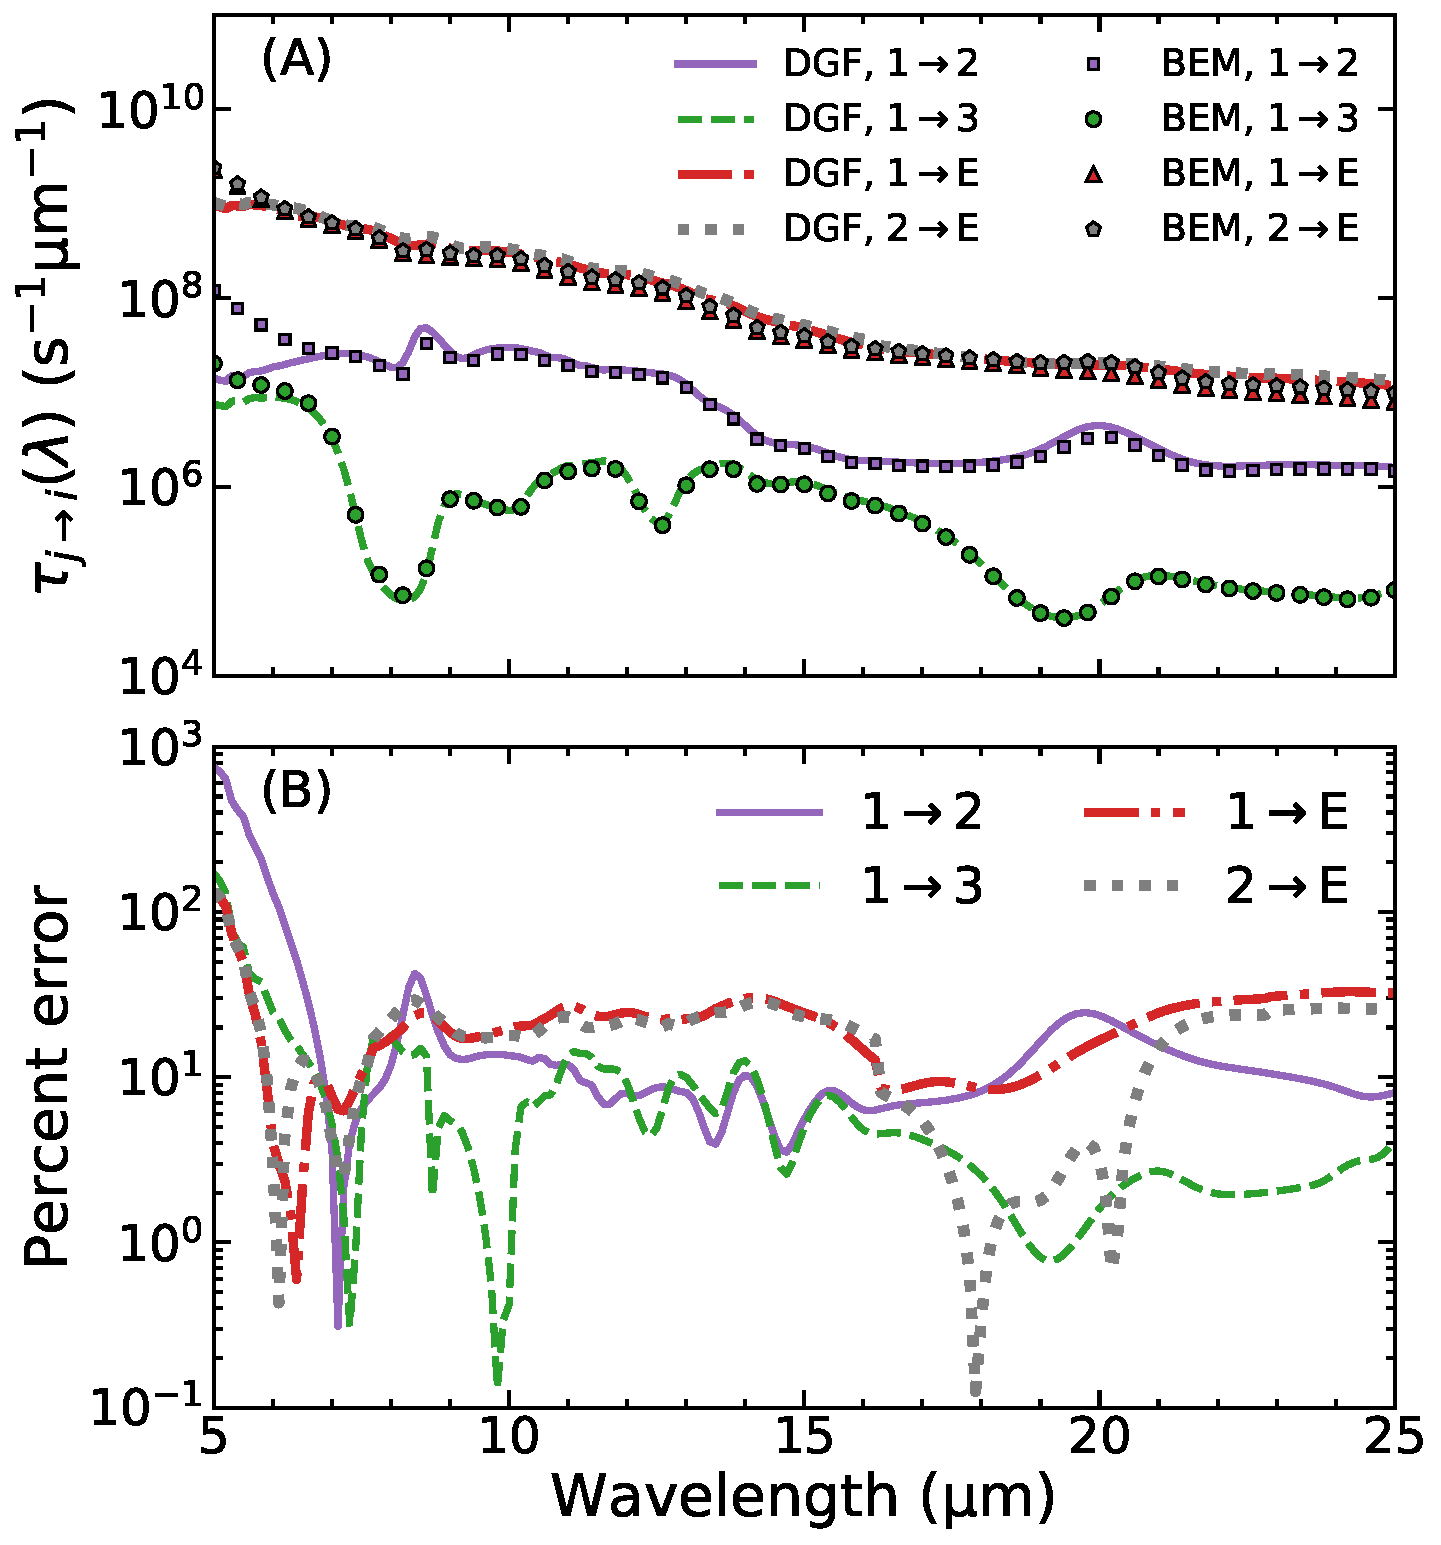
\includegraphics[width=0.8\textwidth]{./Figures/Figure2.pdf}
\caption{\label{fig:ThreeSpheres_SCUFFEM}Cross-validation of DGF and BEM methods. (A) Transmissivity function for energy transfer from source to destination ($j \rightarrow i$) between three identical silicon dioxide spheres with $\rho=10$ \si{\micro\meter} and $D = 1$ \si{\micro\meter}. Values were computed by the DGF (present work) and BEM methods. (B) Magnitude of percent error between two methods in (A).}
\end{figure}

\section{Coated Sphere Results}
%
In this section, all numerical results will be shown for $T=300$ K. Simulated values of spectral and total conductance will be normalized by the conductance between the same two spheres, assuming them to be blackbodies. The spectral conductance between two blackbodies is given by
%
\begin{align}
G_{j \rightarrow i,BB}(\lambda, T) &= \left[ \frac{ \left( \frac{8 \pi^{3} c^{3} \hbar^{2}}{k_{b} T^{2} \lambda^{6}} \right) \exp{\left( \frac{2 \pi \hbar c}{k_{b} T \lambda} \right)} }{ \left[ \exp{\left( \frac{2 \pi \hbar c}{k_{b} T \lambda} \right)} - 1 \right]^{2} } \right] A_{j} F_{j \rightarrow i},
\tag{\ref{eq:SpecCond_BB} revisited}
\end{align}
%
and the total conductance is given by
%
\begin{align}
G_{t,j \rightarrow i,BB}(T) &= \int_{0}^{\infty} G_{j \rightarrow i,BB}(\lambda, T) d\lambda = 4 \sigma T^{3} A_{j} F_{j \rightarrow i},
\tag{\ref{eq:TotalCond_BB} revisited}
\end{align}
%
where $A_{j}$ is the surface area of object $j$, $F_{j \rightarrow i}$ is the radiative view factor from object $j$ to object $i$, and $\sigma=\pi^{2} k_{B}^{4}/60c^{2}\hbar^{3}$ is the Stefan-Boltzmann constant.

\subsection{Dielectric coating atop metal core}

Planar stratified HMMs have previously been investigated for heat transfer applications due to their broadband super-Planckian thermal emission properties.\cite{Guo2012, Guo2013} Though use of non-planar layered media is relatively rare in the study of near-field heat transfer, a thermal MEMS device with a layer of polar material atop a curved chromium sensor has been used in extreme near-field experiments by Kim et al.\cite{Kim2015} It is important to note that a single layer of material does not make the device an HMM. Regardless, our work may still give insight into the behavior of the device. Despite their device having coatings, Kim et al. modeled their curved probe as homogeneous, composed of the polar material only. The authors provided only a \textit{post hoc} justification of this assumption: the seeming agreement between modeled and measured results.

Numerical investigation of heat transfer can shed light on the validity of such an assumption. The simplest test case is to simulate the heat transfer between two identical single-coated spheres. For the simulations here we use a metallic core and a dielectric coating, composed of silver\cite{Yang2015} and silica,\cite{Palik1985} respectively. Varying the spheres' dimensions, the position of the metal/dielectric interface and the separation gap allows for characterization of the impact of dielectric coatings atop metallic cores.

Figure \ref{fig:SpectralConductance} shows the effect of altering the position of the metal/dielectric interface on the spectrum of radiative heat transfer. The coated spheres have an outer radius, coating thickness, and core radius of $\rho$, $t$, and $\rho-t$, respectively. Their geometries are fixed such that $\rho=10$ \si{\micro\meter} and the minimum separation gap is $D=1$ \si{\micro\meter}.

\begin{figure}
\centering
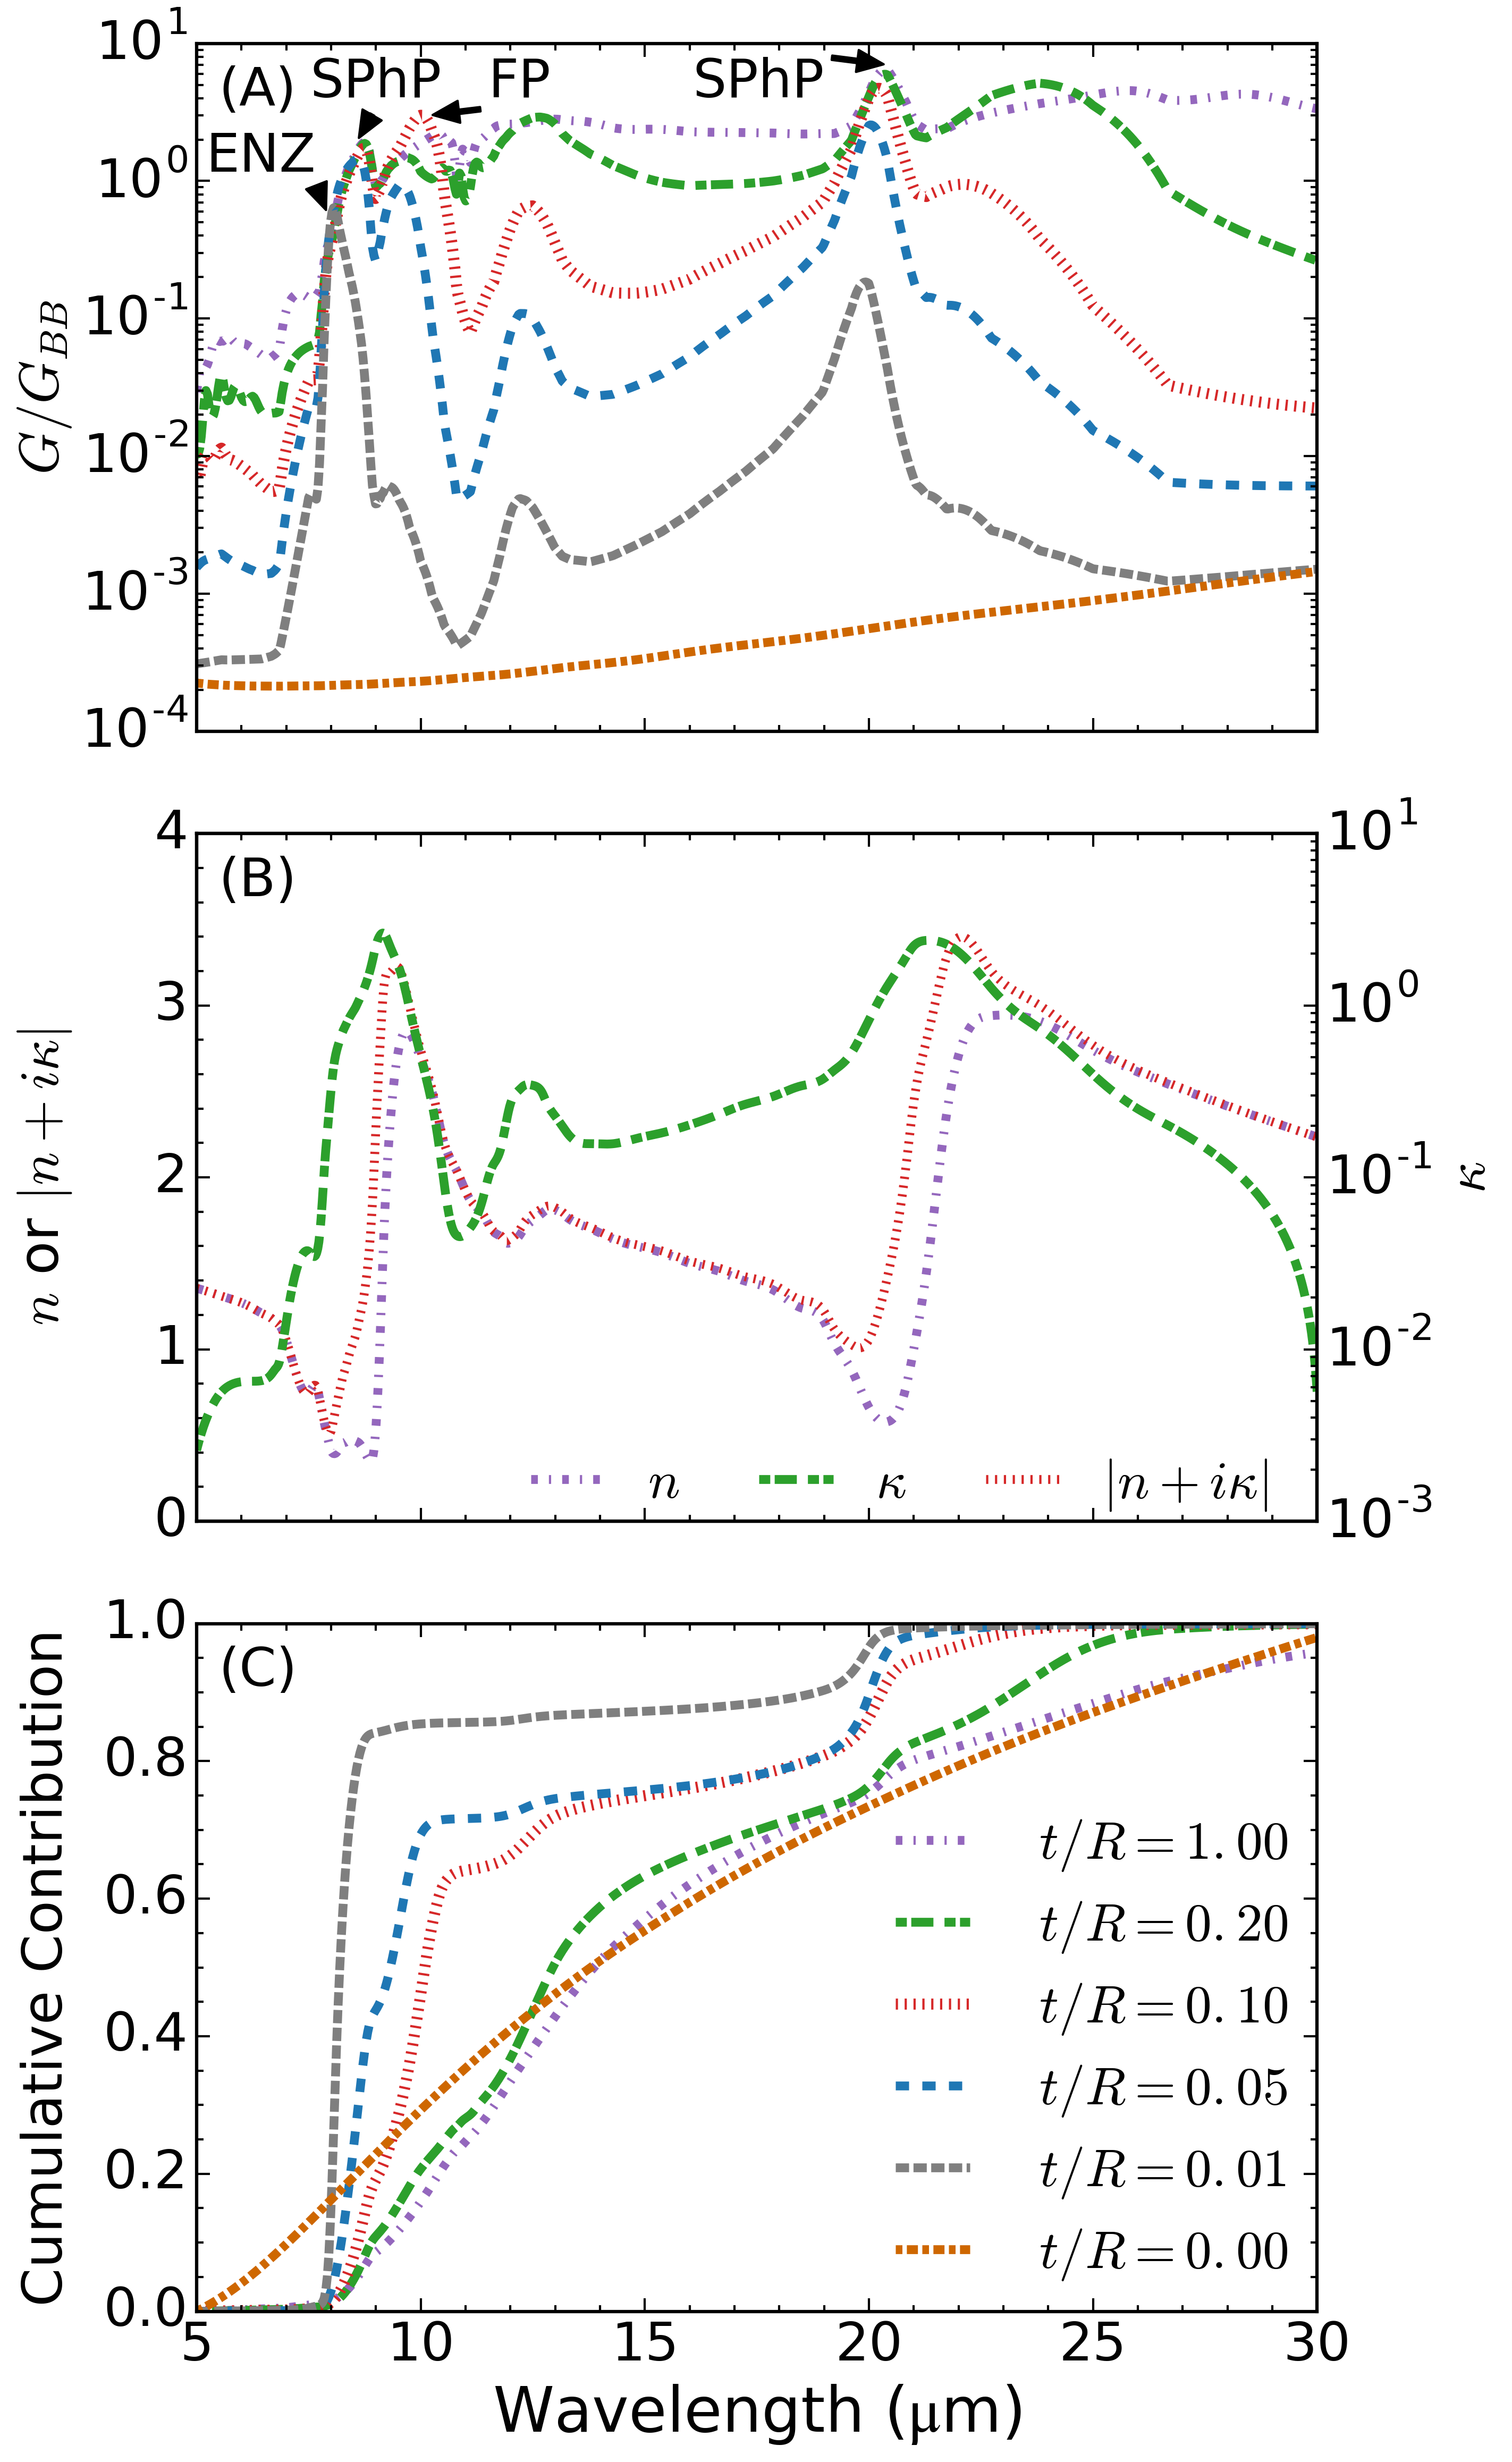
\includegraphics[width=0.75\textwidth]{./Figures/figure2.png}
\caption{\label{fig:SpectralConductance} (A) Spectral conductance between sets of identical coated spheres with varying core/coating interface positions (normalized by that of two blackbody spheres). Spheres have a silver core and silica layer with outer radii of 10 \si{\micro\meter} and minimum separation gap of 1 \si{\micro\meter}. Surface phonon polariton (SPhP), Fabry-Perot (FP), and epsilon near zero (ENZ) peaks are labeled. Legend appearing in (C) also applies to curves appearing in (A). (B) Real ($n$) and imaginary ($\kappa$) components and magnitude ($|n+i\kappa|$) of the complex refractive index of silica. (C) Cumulative spectral contribution to conductance for the curves depicted in (A).}
\end{figure}

The spectral conductance is shown in Fig. \ref{fig:SpectralConductance}(A). For the case of a homogeneous silica sphere ($t/\rho=1$), the result is a relatively wideband distribution of frequencies contributing to the radiative transfer which exactly reproduces the results of previous work. \cite{Narayanaswamy2008} The two well-known surface phonon polariton (SPhP) peaks are present at 8.75 \si{\micro\meter} and 20.3 \si{\micro\meter} [labeled in Fig. \ref{fig:SpectralConductance}(A)]. As the silver core is allowed to grow, the spectrum incrementally changes into the case of two bare silver spheres. Spheres with $t/\rho=0.1$, $0.05$, and $0.01$ exhibit spectral conductances, which appear to be roughly scaled versions of each other, the scaling proportional to the thickness of the coating. 

The sequence in which the spectrum of radiative transfer for silica spheres transitions to that of silver spheres is not uniform across the spectrum. Although the magnitude of the spectral conductance of silver is always lower than that of silica, increasing the proportion of silver to silica may actually increase the spectral conductance for some wavelengths at some intermediate coating thicknesses. This is evident in the spectrum of spheres with $t/\rho=0.2$ at 12.5 \si{\micro\meter} and 23.5 \si{\micro\meter} and $t/\rho=0.1$ at the wavelength of 10 \si{\micro\meter}, where a broad super-Planckian peak, not associated with an SPhP, manifests. At these wavelengths, the conductance of the coated spheres exceeds that of pure silica spheres. 

When a thin layer of polar material (or any material with narrow absorption bands) is coated on a metallic substrate, the wavelength at which the magnitude of the dielectric function (or equivalently the complex refractive index) of the polar material reaches a minimum, $\lambda_{ENZ}$ (ENZ denoting epsilon near zero), takes special significance.\cite{Narayanaswamy2014} At this wavelength alone, the interface between the coating and vacuum behaves as a highly reflective mirror. The interface between the metallic substrate and the thin film is highly reflective at all wavelengths considered here because of the high dielectric function of metals for mid-infrared wavelengths.

Near $\lambda_{ENZ}$, electromagnetic waves experience reflective conditions at both interfaces, leading to a larger number of reflections than at other wavelengths, if the thin film is not too absorptive. The result of a greater number of reflections is the appearance of an optically thicker film. Because amorphous silica has a relatively high damping, these interesting effects manifest themselves in the near field only when the thickness becomes very small. Amorphous silica has a $\lambda_{ENZ}$ point at 7.95 \si{\micro\meter} [see Fig. \ref{fig:SpectralConductance}(B)]. Hence, the stand-alone peak in Fig. \ref{fig:SpectralConductance}(A) for $t/\rho = 0.01$ at 8.06 \si{\micro\meter} is an epsilon near zero mode. As the thickness is increased, this peak can no longer be resolved because of its proximity to a SPhP peak.

Another class of peaks which appears in the spectrum of thermal radiative transfer of coated structures is the Fabry-Perot--like resonance. This type of resonance results from the interference of the multiple reflections of waves within a thin film. Because Fabry-Perot-like resonances require the constructive interference of waves, the location of the peak will drift as the thickness of the coating changes. This type of peak is evident in Fig. \ref{fig:SpectralConductance}(A) for $t/\rho = 0.1$ at 10.0 \si{\micro\meter} and $t/\rho = 0.05$ at 9.55 \si{\micro\meter}.

The cumulative spectral contribution to conductance is shown in Fig. \ref{fig:SpectralConductance}(C). The cumulative contribution at wavelength $\lambda$ is given by 
%
\begin{align}
CSC(\lambda) &= \frac{\int_{0}^{\lambda} d\lambda' G(\lambda',T)}{\int_{0}^{\infty} d\lambda' G(\lambda',T)},
\end{align}
%
where $\lambda'$ is a dummy integration variable. The slopes of the cumulative contribution curves indicate how relatively dominant a wavelength is in contributing to the total conductance. A greater slope indicates a greater relative contribution to the total conductance and vice versa.

The curves for spheres with $t/\rho \ge 0.2$ have relatively small slopes across most wavelengths. This is consistent with the fairly wideband behavior demonstrated in Fig. \ref{fig:SpectralConductance}(A). As $t/\rho$ decreases, however, wavelengths differentiate into two categories: those with nearly zero slope and those with a very steep slope. For $t/\rho =0.10$ and $t/\rho =0.05$, the curves become nearly vertical at the SPhP wavelengths. In the most extreme case, for $t/\rho=0.01$, the curve is nearly vertical at 7.95 \si{\micro\meter} and 19.79 \si{\micro\meter} and nearly horizontal elsewhere. These wavelengths correspond to ENZ points of the silica layer.  If the minimum separation gap between the spheres is decreased, SPhP peaks grow and eventually dominate over ENZ peaks. The dominance of SPhP modes in the extreme near field is made clear in the discussion of Fig. \ref{fig:TotalConductance}.

As we have shown, adding a very thin layer of a material supporting surface polaritons to a metallic substrate creates a selective near-field emitter. (This was already known to be true in the far field.\cite{Granqvist1980, Narayanaswamy2014}) Experimental measurement of spheres with very thin coatings would allow for probing of resonant heat transfer, some of which may be due to SPhPs, while suppressing heat transfer at other wavelengths. Because SPhPs are known to dominate heat transfer between polar materials in the extreme near field, isolating the contributions from SPhPs by using a coated sphere would serve as a superior experimental method compared to measuring the effects of SPhPs with homogeneous spheres as in past experiments.\cite{Narayanaswamy2008a, Shen2009, Guha2012}

Figure \ref{fig:TotalConductance} shows the effect of varying the separation gap between spheres with outer radii of 5 \si{\micro\meter} on total conductance. According to classical radiative transfer, the distance dependence in the far field is due to changes in view factor. Indeed, for gaps such that $D/\rho \ge 2$, all cases are well approximated as graybodies, as indicated by the curves' near-zero slopes. In that regime, the total conductance of spheres of constant radius increases as the fraction of silica increases.

As the separation gap decreases, the conductance between spheres with a silica coating begins to be dominated by the SPhP contributions. At a separation gap such that $D/\rho=0.004$, a coating of just 50 \si{\nano\meter} of silica can achieve 70\% of the conductance of a fully silica sphere. This allows for the creation of spheres with silica-like behavior in the near-field but tunable radiative transfer behavior in the far-field. As a simple rule of thumb, the conductance between two silica coated silver spheres exceeds 70\% of that between two homogeneous silica spheres for $D/t \lesssim 1/4$. For larger gaps, the conductance is more like that of silver.

\begin{figure}
\centering
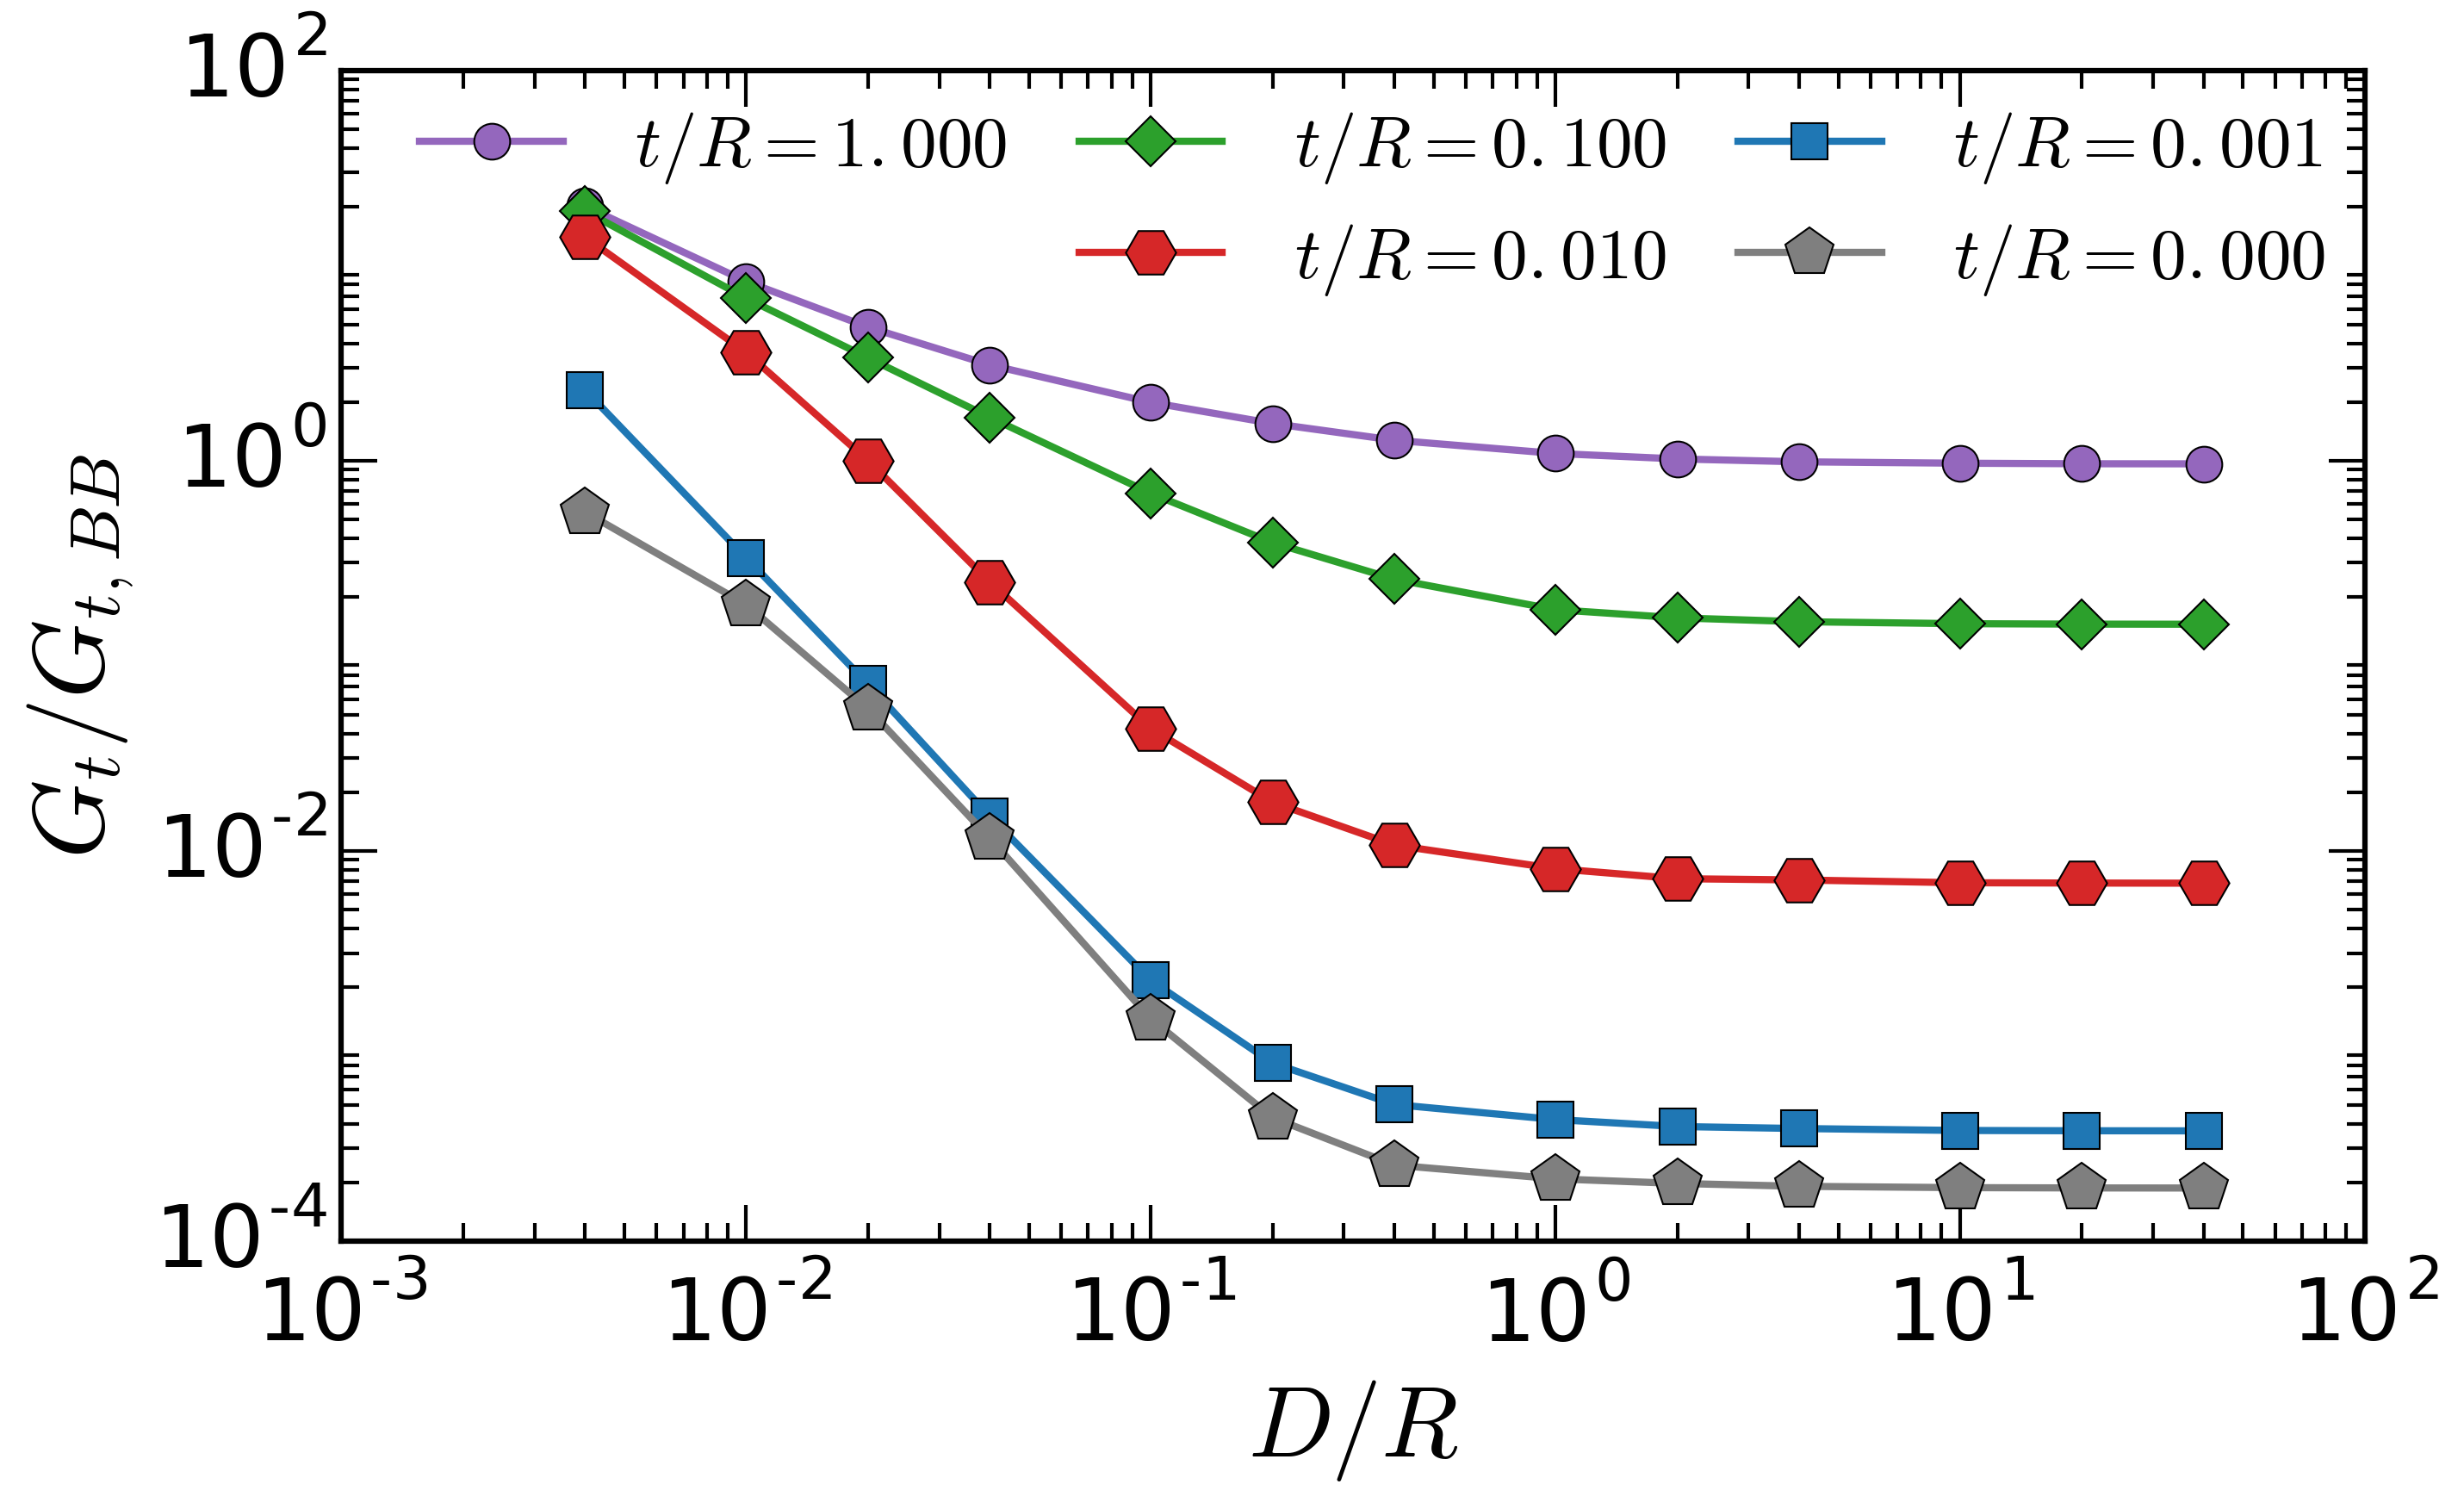
\includegraphics[width=0.8\textwidth]{./Figures/figure3.png}
\caption{\label{fig:TotalConductance} Distance dependence of total conductance between two identical coated spheres. Spheres have a silver core and silica layer with outer radii of 5 \si{\micro\meter}. Total conductance is normalized by that of two blackbodies, and the minimum separation gap is normalized by the outer radii of the spheres.}
\end{figure}

This observation partially validates the assumption made by Kim et al.\cite{Kim2015} Their device had a 100 \si{\nano\meter} silica coating atop an optically opaque chromium thermocouple. Their measurements were performed in the extreme near-field, at gaps ranging from 1 \si{\nano\meter} to 50 \si{\nano\meter}. For the smallest gaps, we have shown that the SPhP contributions will be dominant and modeling the whole body as homogeneous silica is a reasonable approximation. However, should the gaps of interest be larger or the materials not be dominated by SPhPs, more care must be taken to properly approximate near-field thermal radiative transfer of coated bodies.

\subsection{Dielectric coating atop dielectric core}

We observed that the total conductance of the two spheres with dielectric coatings and metallic cores is effectively capped at that of two homogeneous spheres composed of the same dielectric material. A natural question is whether or not two coated spheres can ever exceed the total conductance of two homogeneous spheres which are composed of any of the coated spheres' constitutive materials. Because of the importance of SPhPs in near-field radiative heat transfer, we simulate the conductance between two coated spheres whose cores and coatings both support SPhPs. As shown in Fig. \ref{fig:TwoDielectrics}(A), we simulate identical spheres with beryllia\cite{Palik1985} cores and alumina\cite{Palik1985} coatings, or vice versa, with outer radii of 5 \si{\micro\meter} and a minimum separation gap of 100 \si{\nano\meter}. Those spheres simulated with an alumina coating and a beryllia core such that $0.01 \le t/\rho \le 0.5$ all exceed the total conductance between two homogeneous alumina spheres (which themselves exceed that of two homogeneous beryllia spheres). The maximum occurs at $t/\rho \approx 0.05$. Although spheres with beryllia coatings and alumina cores never exceed the total conductance of homogeneous alumina spheres, they too exhibit a slight local maximum at the same value of $t/\rho$. The maximum total conductance of the coated spheres outperforms homogeneous alumina spheres by 8.5\%.

When looking at the spectral conductance of the homogeneous spheres and the coated sphere with the maximum conductance, it becomes apparent how the coated spheres are able to outperform the homogeneous spheres. As shown in Fig. \ref{fig:TwoDielectrics}(B), the coated spheres exhibit spectral features similar to features found in the spectra of their components. Most importantly, the coated spheres strongly reproduce the SPhP peaks of homogeneous alumina at 12.2 \si{\micro\meter} and 20.8 \si{\micro\meter} while capturing a portion of the enhancement due to the SPhP peak of homogeneous beryllia at 10.0 \si{\micro\meter} (SPhP peaks labeled in Fig. \ref{fig:TwoDielectrics}). This suggests that it may be possible to ``stack" the effect of SPhPs at multiple wavelengths by choosing coatings of materials with spectrally spread SPhP peaks.

\begin{figure}
\centering
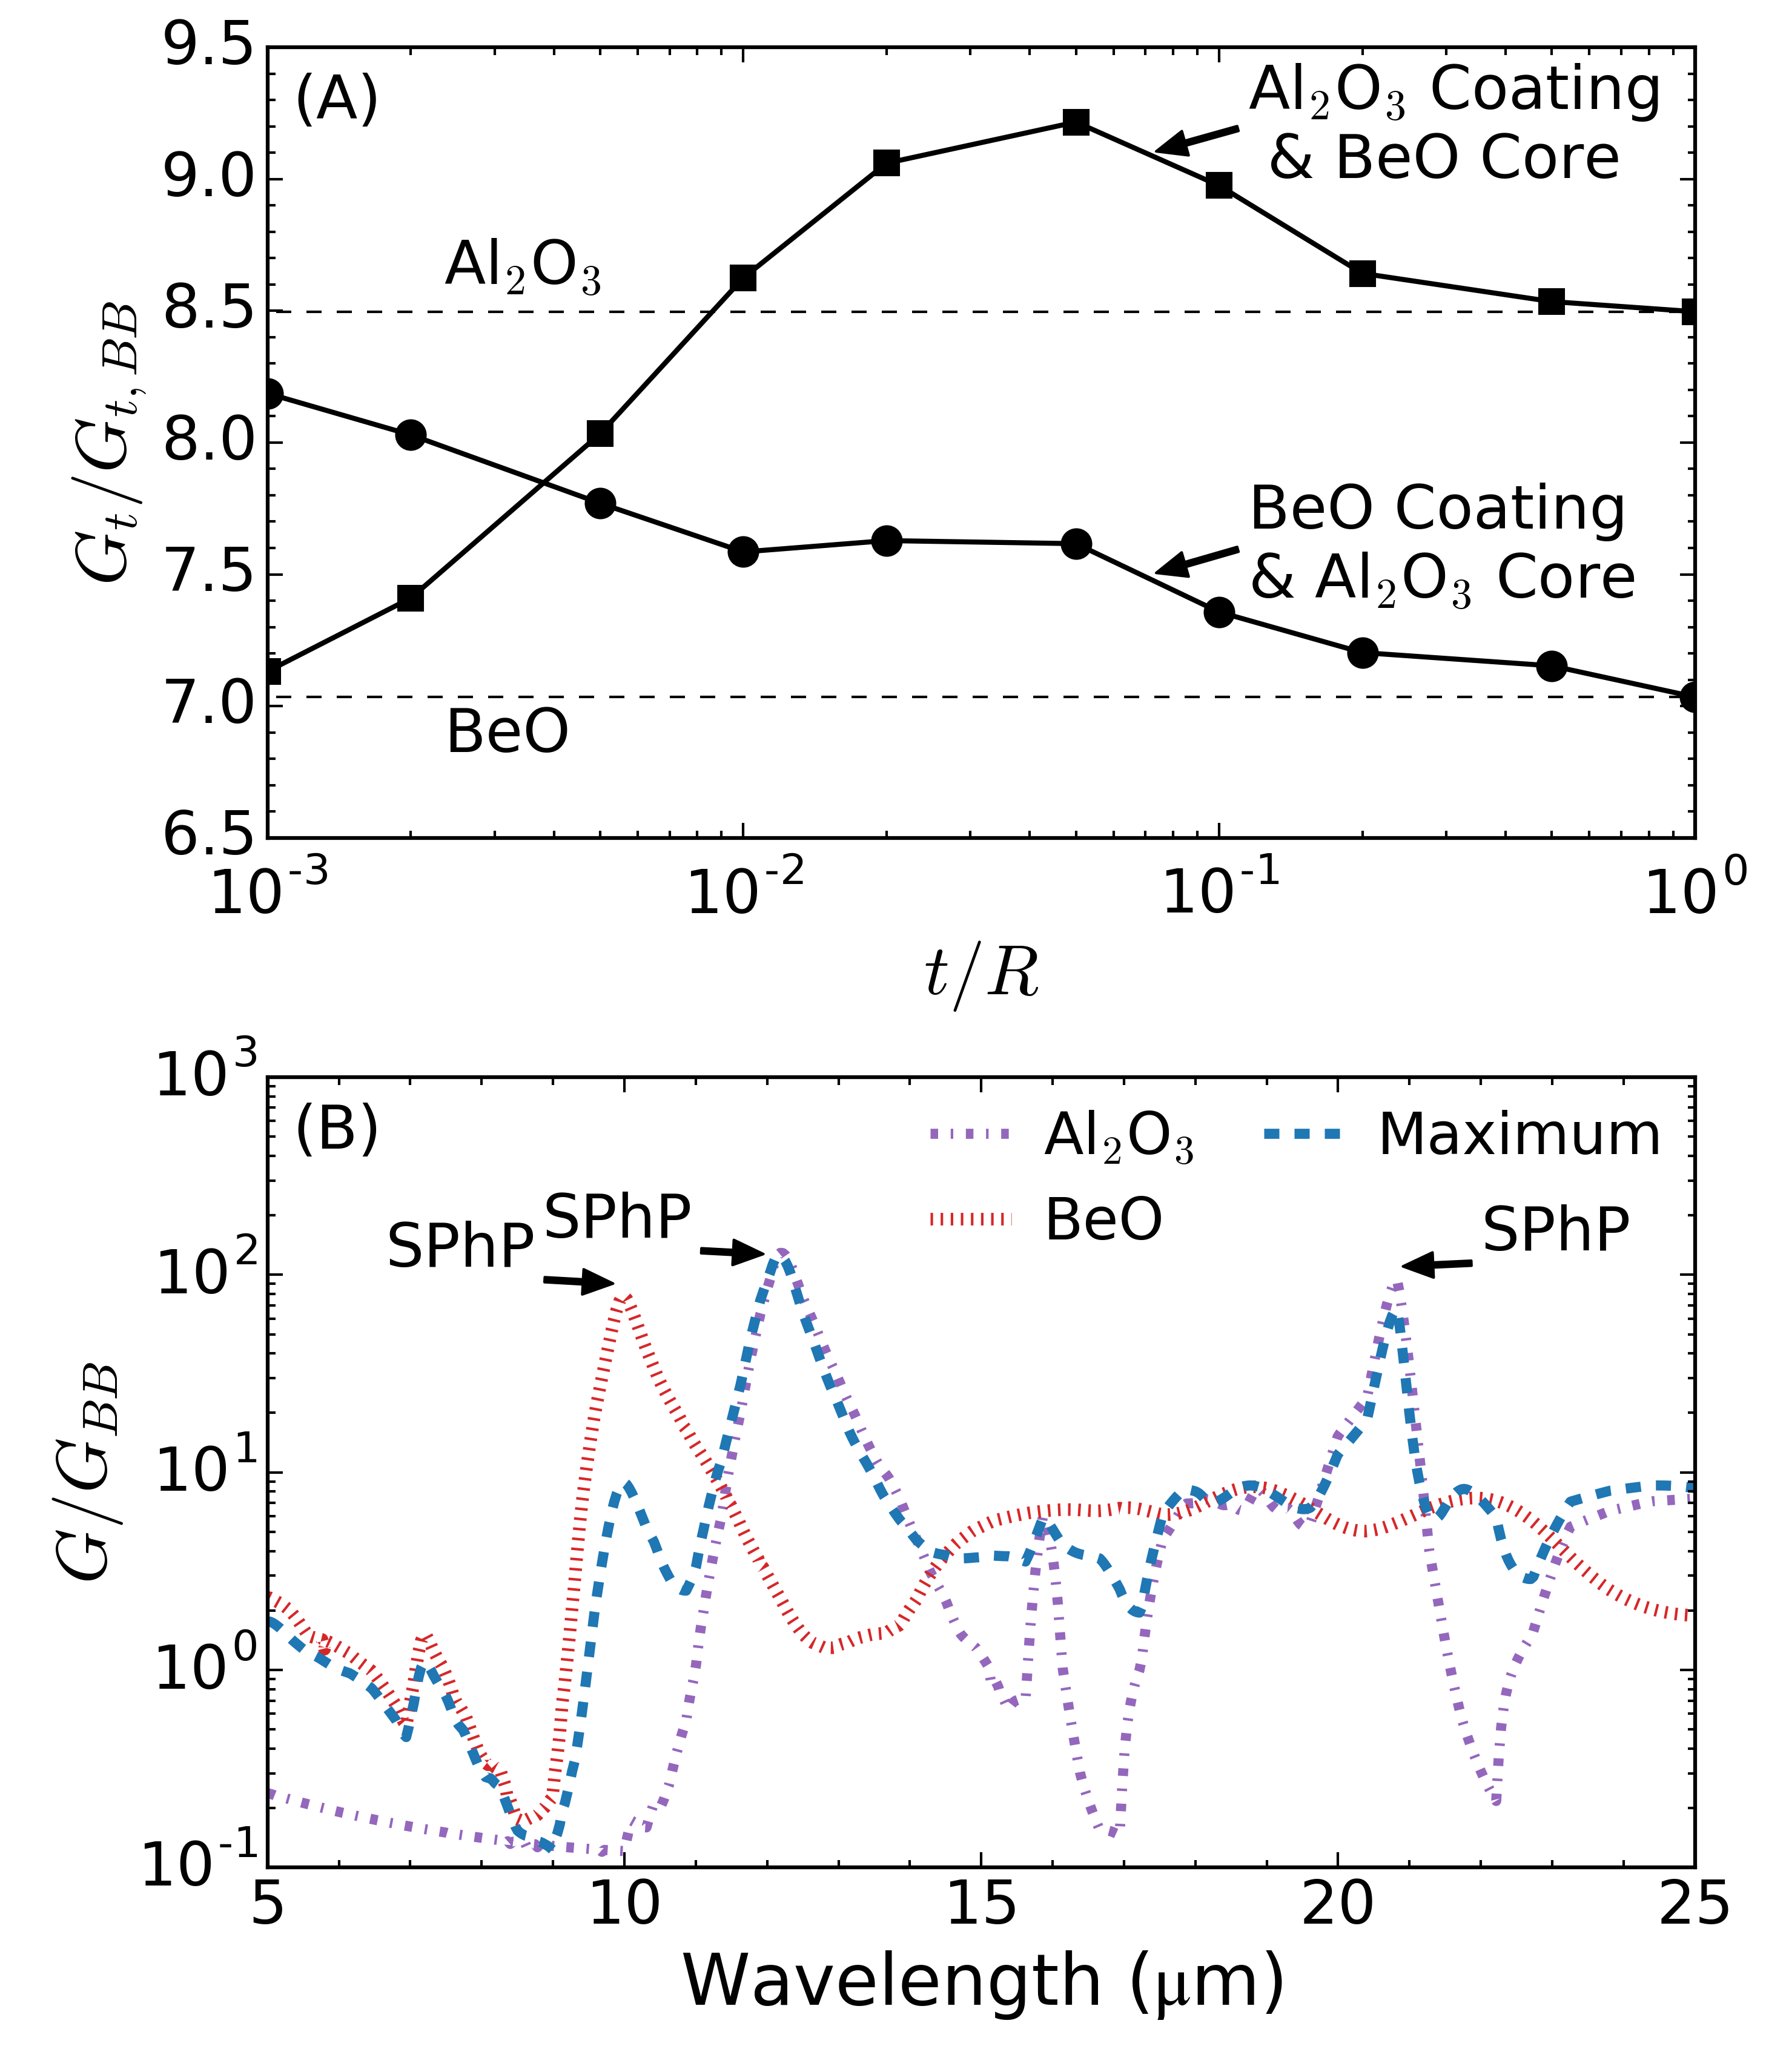
\includegraphics[width=0.8\textwidth]{./Figures/figure4.png}
\caption{\label{fig:TwoDielectrics} (A) Total conductance between two identical coated spheres (normalized by that of two blackbody spheres) as a function of the core/coating interface position. Spheres have a beryllia core and an alumina coating, or vice versa. The spheres have outer radii of 5 \si{\micro\meter} and a minimum separation gap of 100 nm. Dashed lines represent the total conductance of homogeneous beryllia and alumina spheres of the same geometry. Surface phonon polaritonic peaks (SPhP) for the homogeneous spheres are labeled. (B) Spectral conductance of spheres from (A) for homogeneous beryllia, homogeneous alumina, and the coated sphere with the maximum total conductance (alumina coating and beryllia core with $t/\rho=0.05$).}
\end{figure}
\section{Implications for NFRHT Experiments}
%
Until the recent advances in NFRHT between MEMS devices,\cite{Song2016, Cui2017, Fiorino2018} experiments measuring NFRHT with sub-micron gaps were performed in the microsphere-plane configuration, much like the configurations used in Casimir and van der Waals force experiments.\cite{Lamoreaux1997, Mohideen1998, Roy1999, Harris2000} Recent experimental work investigating the Casimir force\cite{Garrett2018} demonstrates that sphere-sphere geometries are also a feasible configuration to investigate NFRHT. To better understand how such a sphere-sphere NFRHT experiment would work, we must first understand how sphere-plane experiments have been performed.

In past sphere-plane NFRHT experiments,\cite{Rousseau2009,Shen2009} experimenters attached the sphere to a bimaterial microcantilever. Bimaterial cantilevers, such as atomic force microscopy cantilevers, are extremely sensitive calorimeters which deflect with any change in temperature. The planar substrate was fixed at a temperature, either passively to the ambient or heated to a temperature above ambient. If the substrate was fixed at ambient temperature, then the sphere was heated using a laser to create a temperature difference between the two objects. Otherwise, the heated substrate supplied the temperature difference.

The sphere was initially located at some distance above the substrate, typically between 2.5 \si{\micro\meter} and 10 \si{\micro\meter}. The separation between the sphere and substrate was then decreased until contact was made. Due to surface imperfections and the resolution of the system controlling the separation distance, the minimum distance achievable was approximately 30 \si{\nano\meter} in Refs. \citenum{Shen2009} and \citenum{Rousseau2009}.

As a sphere lowers, its temperature changes, which results in a change in deflection angle of the cantilever. The change in deflection angle, unlike the temperature, is the experimental parameter which can actually be measured. Change in deflection angle must be related to the change in conductance between the two objects by using a thermal model. Because the measurement can only measure changes in deflection angle, the experiment is sensitive only to changes in total conductance from its value at the initial (maximum) separation distance to its value at its some later time.

The thermal model used to infer sphere-plane conductance must account for all means of heat transfer occurring. Critically, it must reflect the fact that the sphere-plane system is really a sphere-plane-environment system with exchanges of thermal energy between both objects and their environment. Prior works employing sphere-plane geometries have used a variety of approaches to account for heat transfer to the environment. For example, some works have used Mie theory to compute sphere-environment conductances,\cite{Narayanaswamy2008a} assumed a constant but unnamed value,\cite{Shen2009} ignored environmental heat transfer effects all together,\cite{Rousseau2009, Guha2012} or not reported their treatment of far-field radiation at all.\cite{Kim2015} Any improper treatment of the sphere-environment conductance will introduce a systematic error.

\begin{figure}
\centering
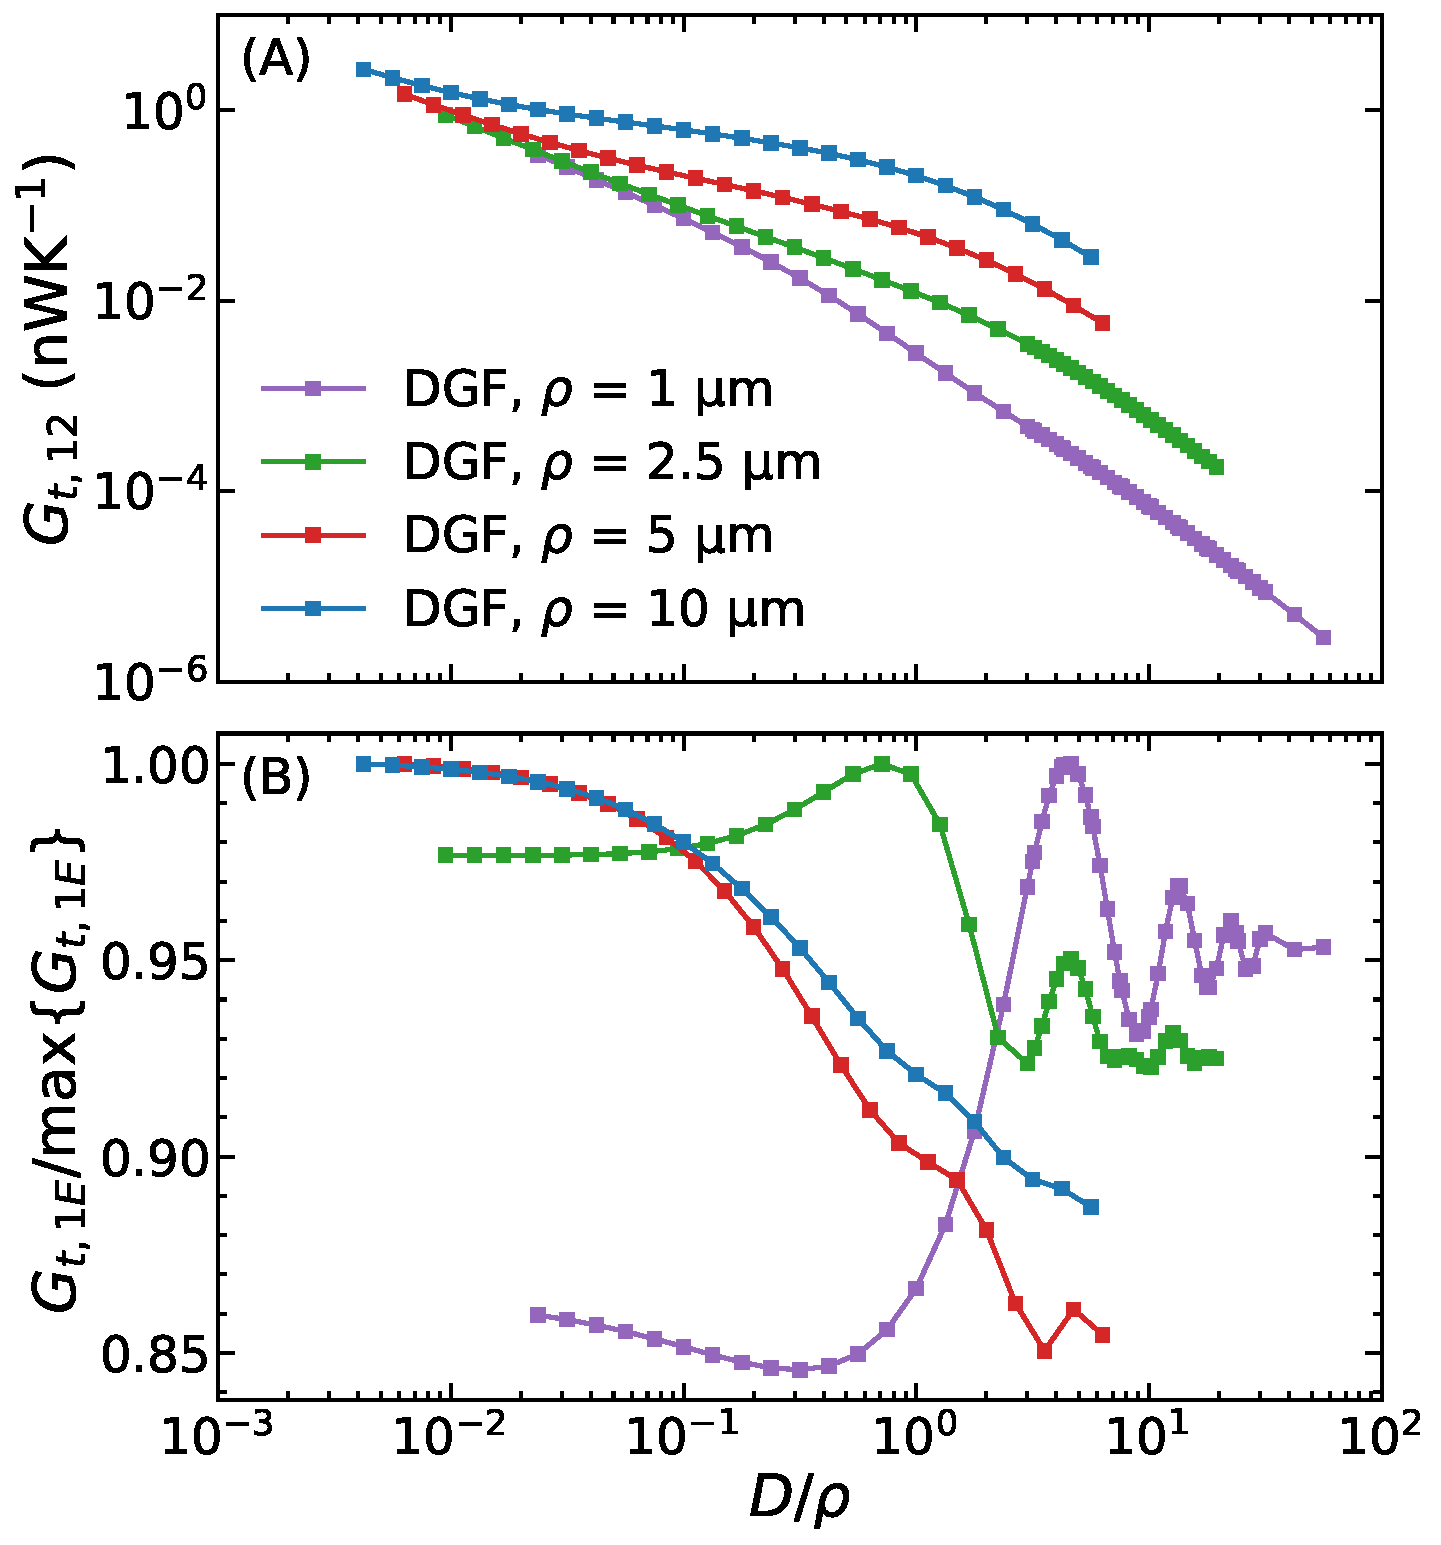
\includegraphics[width=0.8\textwidth]{./Figures/Fig_MockExperimentDissertation.pdf}
\caption{\label{fig:DistanceDependence} Total conductance in a system of two identical silicon dioxide spheres with outer radii of 10 \si{\micro\meter}. The legend in (A) is common to both subfigures. (A) Sphere-sphere conductances determined by DGF method. (B) Sphere-environment conductances (normalized by the maximum value of each curve) predicted by the DGF method. The oscillations present for the smallest spheres are signs of diffraction.}
\end{figure}

To investigate the magnitude of that error in a potential sphere-sphere experiment, we simulate the NFRHT for two identical silicon dioxide spheres with outer radii of 1, 2.5, 5, and 10 \si{\micro\meter}. Figure \ref{fig:DistanceDependence}A shows sphere-sphere conductances and Fig. \ref{fig:DistanceDependence}B shows normalized sphere-environment conductances. The legend in Fig. \ref{fig:DistanceDependence}A is common to the entire figure. As expected, the sphere-sphere conductances determined by the DGF method show a super-Planckian monotonic increase in the near-field. More interestingly, it is readily apparent from Fig. \ref{fig:DistanceDependence}B that the character of the sphere-environment conductances has a strong size dependence. The smallest spheres show strong signs of diffraction for large separation distances, reminiscent of recent work involving point particles (see Fig. 8 of Ref. \citenum{Asheichyk2017}). The smallest sphere ($\rho$ = 1 \si{\micro\meter}) actually shows a decrease in sphere-environment conductance with decreasing distance. The next smallest ($\rho$ = 2.5 \si{\micro\meter}) shows an eventual increase over its far-field value, though it has a global maximum at an intermediate gap. The largest spheres ($\rho$ = 5 \si{\micro\meter} and 10 \si{\micro\meter}) show near-monotonic increases and a maximum value at the smallest gap simulated. This demonstrates that the intense electric and magnetic fields between objects which contribute to NFRHT can dampen or enhance far-field emission, with a seeming size dependence. The one common trend is that all sphere-environment conductances eventually level off for sufficiently small $D/\rho$.

The fact that the curves level off is key to taking a valid measurement of sphere-sphere conductance using a cantilever. Since cantilevers are sensitive to changes of conductance from the initial point to the final, starting an experiment at a sufficiently small initial separation gap should result in no change in the sphere-environment conductance and an isolation of the sphere-sphere conductance. The value of $D/\rho$ required by each silicon dioxide sphere to have a maximum relative error of approximately 5\% are given in Table \ref{tab:ErrorInSphereSphere}. Further work must be devoted to determining a universal criterion. The current results suggests that smaller spheres will allow for a larger range of separation distances to be probed. This is contrary to the many large spheres used in sphere-plane experiments.\cite{Rousseau2009,Shen2009}

\begin{table}
	\caption{\label{tab:ErrorInSphereSphere}Initial values of $D/\rho$ which will ensure a relative error of approximately 5\% or less in a hypothetical sphere-sphere experiment.}
	\begin{center}
		\renewcommand{\arraystretch}{1.15}
		\setlength{\tabcolsep}{0.10cm}
		\begin{tabular}{ccccccccc}
			\hline 
			\multicolumn{1}{c}{$\rho$ (\si{\micro\meter})} &
			\multicolumn{1}{c}{$D_{0}/\rho$} \\
			\hline
			%
			1 & 1.00 \\ 
			2.5 & 0.40 \\
			5 & 0.10 \\
			10 & 0.06 \\
			\hline
		\end{tabular} 
	\end{center}
\end{table}

It is my hope that this work may spur other researchers to modify their methodologies and reporting practices to reflect the importance of heat transfer to the environment in NFRHT experiments. Additionally, by better quantifying far-field heat transfer, the possibility is left open of closely studying other phenomena that cause NFRHT to deviate from idealized behavior, for example surface roughness.\cite{Kruger2013, Chen2015} % Done X
\chapter[Summary and Future Work][Summary and Future Work]{Summary and Future Work} \label{ch:Summary}

\section{Main Contributions}
%
\begin{enumerate}
\item \textit{NFRHT Between Layered Spheres:} I developed the first numerically exact model for NFRHT between two coated spheres and used it to investigate the impact of coatings on the spectrum of NFRHT. I observed a number of interference-based peaks in the spectrum of NFRHT between two metallic spheres with polar material coatings. The peaks were reminiscent of my earliest work involving NFRHT between two homogeneous silicon carbide spheres.\cite{Czapla2014} These similarities were due to silicon carbide's low absorption allowing waves to enter into each sphere, reflect off the backside and constructively/destructively interfere with other waves, in a similar fashion to waves entering a thin coating and reflecting off the metallic core. I also showed that layered spheres composed of different materials which support SPhPs can result in enhanced NFRHT, above that of either material alone. (See Refs. \citenum{Czapla2017}, \citenum{Czapla2014}, and \citenum{Czapla2017b}.)
\item \textit{NFRHT in Chains of Spheres:} I extended my two sphere work to include any number of coated spheres in a linear chain. I can simulate both sphere-sphere and sphere-environment radiative transfer. Using this work, I was able to issue a warning regarding the distance-dependence of sphere-environment heat transfer to any experimentalist who wishes to conduct sphere-sphere NFRHT experiments using a microcantilever. I also proposed a solution to mitigate the potential risk. Furthermore, I moved software development to GitHub\cite{Narayanaswamy2018} to lower the barrier of entry for other researchers. (See Ref. \citenum{Czapla2018}.)
\item \textit{New Optical Properties:} I published the first broadband optical data for PDMS in the mid-infrared portion of the electromagnetic spectrum. I used those properties to explore the potential of PDMS for radiative cooling applications, another situation that requires tailoring the spectrum of radiative transfer, and demonstrated numerically that PDMS thin films atop aluminum substrates could theoretically reach equilibrium temperatures of 12\si{\celsius} below ambient when exposed to the night sky. (See Refs. \citenum{Srinivasan2016} and \citenum{Czapla2017a}.)
\end{enumerate}


\section{Future Work}
%
\begin{enumerate}
\item \textit{Sphere-Plane Heat Transfer:} Otey et al.\cite{Otey2011} computed the NFRHT between a homogeneous sphere and substrate using a method analogous to the interior method. In doing so, they translated back and forth between vector spherical and cylindrical (required for the plane) waves. It would be interesting to see if the same result could be obtained using an exterior method approach and asymptotic expressions for the spherical Bessel and Hankel functions in the limit as one sphere gets very large. Previous work in the Swamy Group by Sasihithlu and Narayanaswamy\cite{Sasihithlu2014} considered only homogeneous spheres with large size disparity ($\rho_{2} \lesssim 40 \rho_{1}$), not a true $\rho_{2}/\rho_{1} \rightarrow \infty$ case, and requires a convergence analysis to prove that the sphere-sphere NFRHT reaches a steady value which can approximate sphere-plane NFRHT. By taking the approach of Ref. \citenum{Sasihithlu2014}, we should get accurate sphere-environment heat transfer but perhaps not an accurate plane-environment heat transfer. My proposed method should bypass those shortcomings and give access to NFRHT between coated objects in the process.
\item \textit{Higher-Order Discrete Dipole Approximations:} The method outlined in this work should reproduce the discrete dipole approximation (DDA) for two spheres when their radii are small and $l_{\mathrm{max}} = \nu_{\mathrm{max}} = 1.$ Firstly, this should be verified. Secondly, the linear system of scattered field coefficients should be solved explicitly in the case of $l_{\mathrm{max}} = \nu_{\mathrm{max}} =2, 3, 4,... $ until it is no longer feasible. This would provide higher order corrections which could yield DDA models applicable to larger spheres.
\item \textit{Scattered Field Coefficient Bottleneck:} The greatest bottleneck in calculating NFRHT between closely-spaced wavelength-sized spheres is solving for the scattered field coefficients using their linear system. The number of terms for convergence is too great when the spheres are large, very close, or very far. Examining the results of the higher-order DDA could shed insight into a solution to the linear system which doesn't require matrix inversion. Richardson extrapolation also has the potential to accelerate the convergence of the infinite series.
%\item \textit{NFRHT Python Library:} The NFRHT community would benefit greatly if it could coallesce around a common set of open-source numerical tools. Could include future innovations such as... 
\item \textit{Experimental Validation:} As of yet, no two sphere NFRHT experiments have taken place, let alone multiple-body experiments. Experimental NFRHT has lagged behind theoretical NFRHT, and that mismatch should be corrected, both to validate my models and to innovate on existing experimental techniques so we can move toward producing devices which exploit NFRHT phenomena.
\end{enumerate}


%Coding - service to the community. Python library that can translate between all systems. Precompiled Fortran or C code in a python library. move beyond chain. Include common approximations and dielectric functions. Basically, become a software engineer.

%Cylinder-cylinder exterior method. Mostly for completeness.

%Using chain of progressively smaller spheres as a proxy for a sharp tip over a surface (large sphere)

 % Done X

\appendix

\SingleSpacing
\bibliography{./library}

\DoubleSpacing
\chapter[Fresnel Coefficients][Fresnel Coefficients]{Fresnel Coefficients}\label{ap:FresnelCoefficients}

\section{Background}
%
The Fresnel coefficients, $r^{(\alpha)}_{ij}$ (where $\alpha$ is the polarization), give the ratio of electric field before and after the reflection off a planar interface. The Fresnel coefficients depend on wavelength (through the optical properties), the angle of incidence, and the polarization of light. The polarization (essentially orientation) of light is said to either be $s$ (also called transverse electric, TE, or $\perp$) or $p$ (also called transverse magnetic, TM, or $\parallel$). In some sense, the orientation of the fields is arbitrary and two main conventions exist in the literature for the $p$ polarization. In this work, we will follow the convention of Hecht.\cite{Hecht2017} The main difference is that, for the convention used in this work, $r^{(p)} = - r^{(s)} $ at normal incidence. In the opposing convention, the two quantities are equal. A diagram of the convention used here appears in Fig. \ref{fig:FieldConvention}.

One difference between the present treatment and that of Hecht is that we will not use angles directly when examining angles of incidence. For complex refractive indices, Snell's law predicts complex angles, which I find distasteful. Instead, we will use the in-plane component of the wavevector, $k_{\rho}$, to indicate angles. The main advantage is that $k_{\rho}$ stays constant and real in all media. It may be related to the angle of incidence by $k_{\rho} = (2 \pi /\lambda) \cos{\theta}$. A diagram of the components of the wavevector can be seen in Fig. \ref{fig:FieldConvention}A.

\begin{figure}
\centering
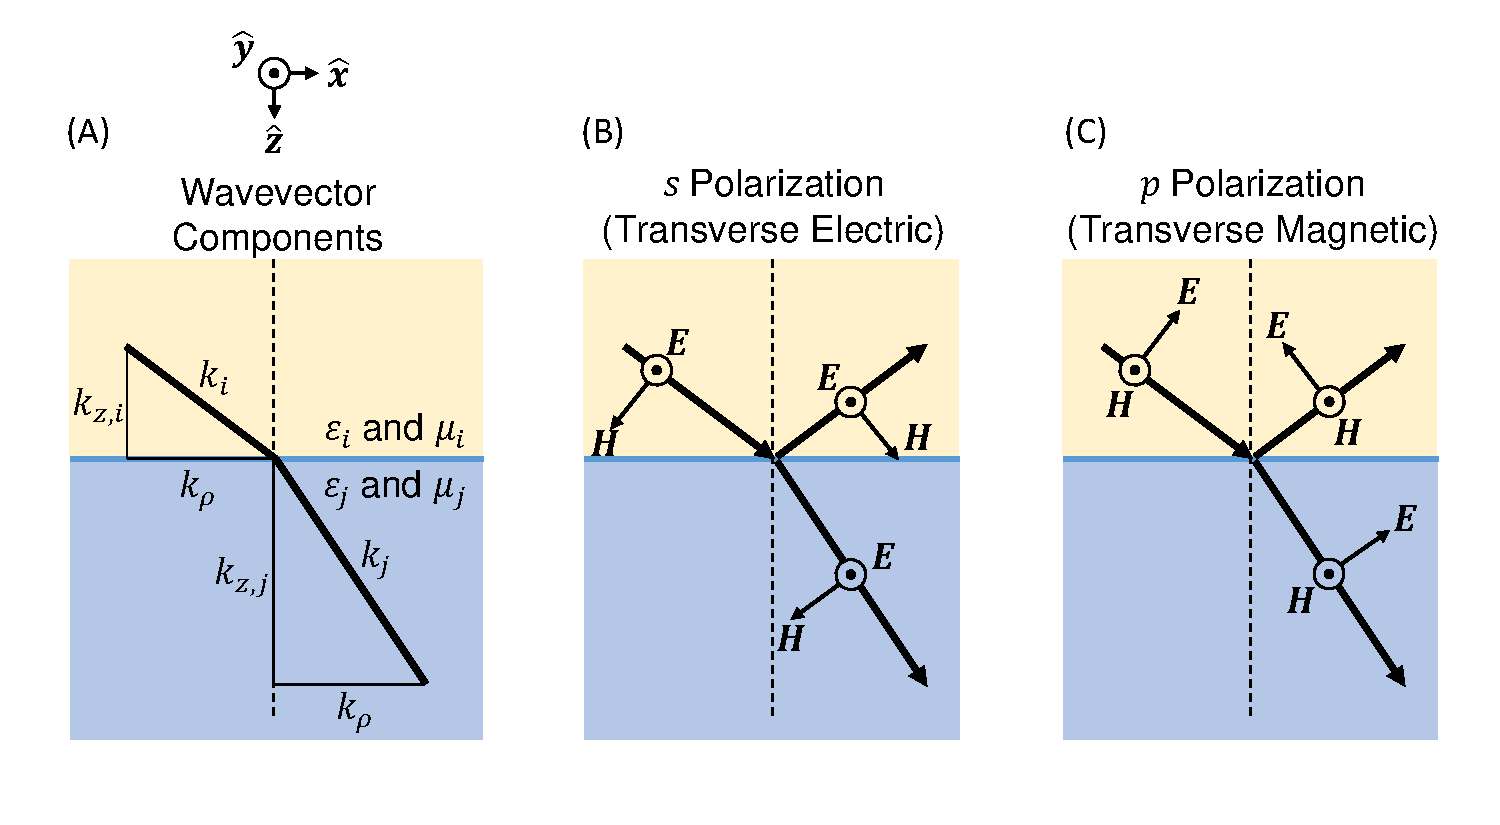
\includegraphics[width=1.0\textwidth]{./Figures/ReflectionConvention.pdf}
\caption{\label{fig:FieldConvention}(A) Diagram of wavevector components and optical properties. (B) Diagram showing orientation of electric and magnetic fields for reflection of $s$ polarization light. (C) Diagram showing orientation of electric and magnetic fields for reflection of $p$ polarization light. }
\end{figure}

\section{Reflection Coefficients} 
%
The Fresnel coefficients between media $i$ and $j$ are given by
%
\begin{subequations}
\begin{align}
r_{i,j}^{(s)} &= \frac{ \frac{k_{z,i}}{\mu_{i}} - \frac{k_{z,j}}{\mu_{j}} }{ \frac{k_{z,i}}{\mu_{i}} + \frac{k_{z,j}}{\mu_{j}} } \\
r_{i,j}^{(p)} &= \frac{ \frac{k_{z,i}}{\varepsilon_{i}} - \frac{k_{z,j}}{\varepsilon_{j}} }{ \frac{k_{z,i}}{\varepsilon_{i}} + \frac{k_{z,j}}{\varepsilon_{j}} }
\end{align}
\end{subequations}

\subsection{Reflectance}
%
Commonly in optics problems, the ratio of electric fields is not a directly useful quantity. Instead, the ratio of electric field intensities is more useful. That ratio is called the reflectance, and is given by
%
\begin{equation}
R_{i,j}^{(\alpha)} = \left| r_{i,j}^{(\alpha)} \right|^{2}
\end{equation}
%
where $\alpha =$ $s$ or $p$.

\subsection{Stratified Media}
%
When a planar medium has multiple planar layers, an effective Fresnel coefficient can be determined. This is typically done using a transfer matrix method\cite{Katsidis2002, Troparevsky2010} or using the Airy formula,\cite{Airy1833, Kaushik1997, Jen2001, Narayanaswamy2013b} which is commonly determined by counting partial wave contributions to reflection. The Airy formula can be used recursively to account for an arbitrary number of layers. It is given by
%
\begin{equation}
\widetilde{r}_{i,i+1}^{(\alpha)} = \frac{r_{i,i+1}^{(\alpha)} + \widetilde{r}_{i+1,i+2}^{(\alpha)} \exp{\left( 2i k_{z,i+1} d_{i+1} \right)} }{ 1 + r_{i,i+1}^{(\alpha)} \widetilde{r}_{i+1,i+2}^{(\alpha)} \exp{\left( 2i k_{z,i+1} d_{i+1} \right)} } 
\end{equation}
%
where $d_{i}$ is the thickness of layer $i$. The recursion is terminated when a semi-infinite half-space is encountered by using a regular Fresnel coefficient in place of the effective one.  % Done X
\chapter[Classical Radiative Transfer][Classical Radiative Transfer]{Classical Radiative Transfer} \label{ap:CRT} \allowdisplaybreaks

\section{Emissive Power of a Blackbody}
%
Define the quantity $e_{\lambda}$ as the monochromatic emissive power (with units of \si{\watt\per\square\meter\per\meter}), which gives the flux of energy radiated from a surface at a given wavelength and temperature. Then 
%
\begin{equation}
e(T) = \int_{0}^{\infty} e_{\lambda}(\lambda, T) d\lambda
\end{equation}
%
gives the total energy flux emitted by the surface at a given temperature. Planck's blackbody law gives $e_{\lambda, BB}$, the monochromatic emissive power of a blackbody, as
%
\begin{equation}\label{eq:BlackBody_Power}
    e_{\lambda, BB}(T,\lambda) = \frac{2 \pi h c^{2}}{\lambda^{5}} \frac{1}{\exp{\left( \frac{hc}{\lambda k_{B}T} \right)} -1}
\end{equation}
%
where $h$ is Planck's constant, $c$ is the speed of light in vacuum, $\lambda$ is the wavelength in vacuum, $k_{B}$ is Boltzmann's constant, and $T$ is the thermodynamic temperature. Integrating to get the total emitted power yields
\begin{equation} \label{eq:StefanBoltzmannLaw}
e_{BB}(T) = \int_{0}^{\infty} e_{\lambda, BB}(\lambda, T) d\lambda = \sigma T^{4}
\end{equation}
%
where $\sigma = 2 \pi^{5} k_{B}^{4}/( 15 c^{2} h^{3} )$ is the Stefan-Boltzmann constant. This is the Stefan-Boltzmann law.

\section{Emissivity}
%
Real objects do not emit exactly like blackbodies, so it is useful to benchmark a real object's emission against that of a blackbody. The ratio of a real object's monochromatic emissive power to that of a blackbody is called the object's spectral emissivity, $\epsilon_{\lambda}$. It is given by $\epsilon_{\lambda} = e_{\lambda} / e_{\lambda, BB}$. Another useful quantity is the total emissivity, which gives the ratio of an object's total emitted power to that of a black body, and is given by
%
\begin{equation}
\epsilon = \frac{e(T)}{e_{BB}(T)} = \frac{ \int_{0}^{\infty} e_{\lambda}(T) d\lambda }{ \int_{0}^{\infty} e_{\lambda,BB}(T) d\lambda } = \frac{ \int_{0}^{\infty} \epsilon_{\lambda} e_{\lambda,BB}(T) d\lambda }{ \int_{0}^{\infty} e_{\lambda,BB}(T) d\lambda } = \frac{ \int_{0}^{\infty} \epsilon_{\lambda} e_{\lambda,BB}(T) d\lambda }{\sigma T^{4}}
\end{equation}


\section{View Factor}
%
The view factor, $F_{i \rightarrow  j}$, is the proportion of rays of light that are emitted diffusely (isotropically) from surface $i$ that strike surface $j$. It is given by the double integral
%
\begin{equation}\label{eq:ViewFactor}
	A_{i} F_{i \rightarrow j} = \int_{A_{i}} \int_{A_{j}} \frac{ \cos{\theta_{i}} \cos{\theta_{j}} }{ \pi S^{2} } dA_{i}dA_{j}
\end{equation}
%
where $A$ is the surface area of an object and $\theta$ and $S$ are configuration parameters which are defined in Fig. \ref{fig:ViewFactor}. The view factor has two very important properties: $A_{i} F_{i \rightarrow  j} = A_{j} F_{j \rightarrow i}$ (which becomes readily apparent by swapping instances of $i$ and $j$ in Eq. \ref{eq:ViewFactor}) and $\sum_{j} F_{i \rightarrow  j} = 1$ (which is a mathematical statement that that all emitted rays must go somewhere).

\begin{figure}
\centering
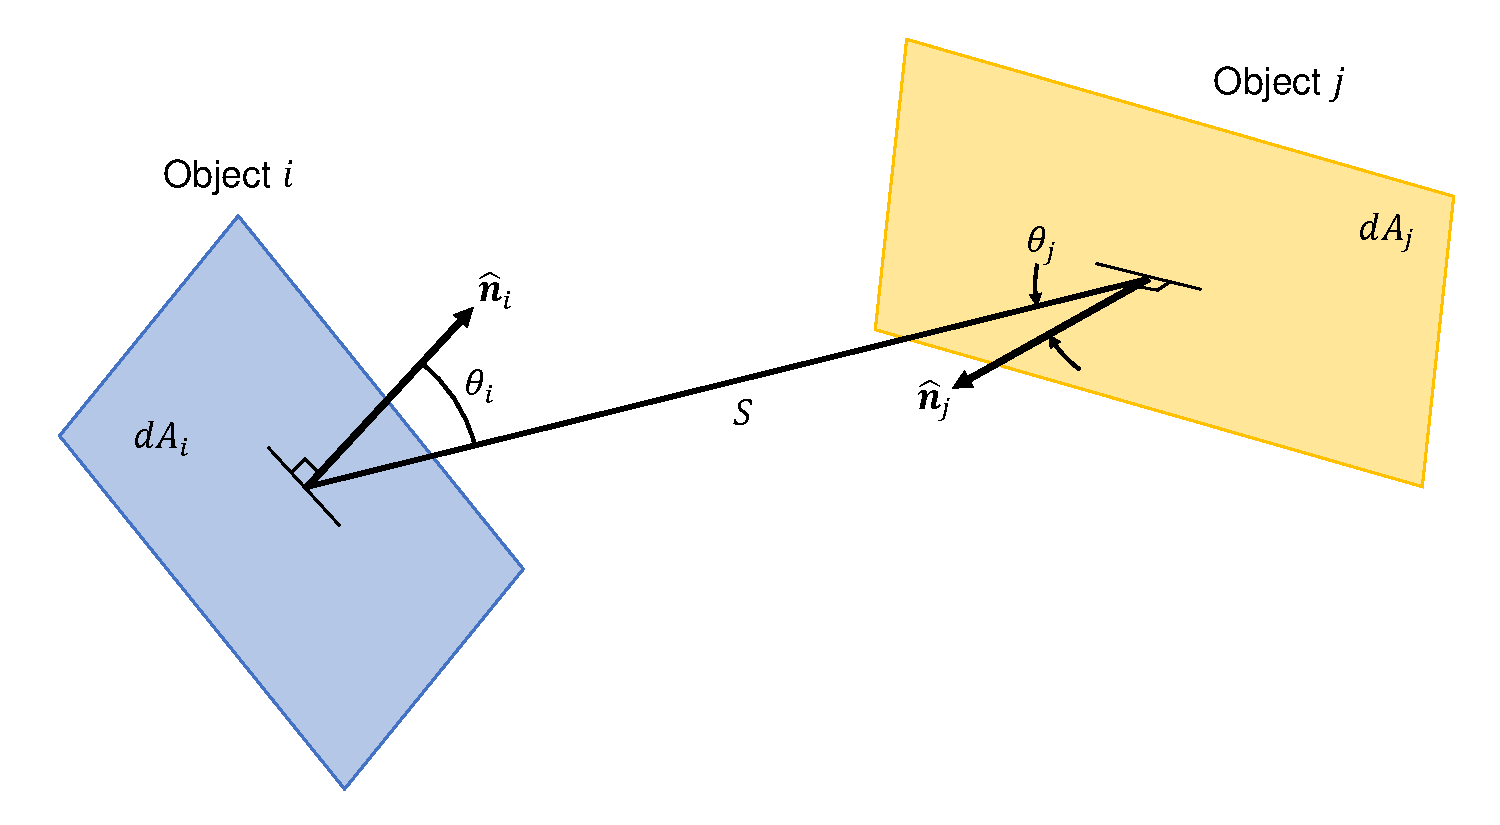
\includegraphics[width=0.8\textwidth]{./Figures/ViewFactor.pdf}
\caption{\label{fig:ViewFactor}Diagram of geometric parameters necessary to compute a view factor.}
\end{figure}


\section{Radiative Heat Transfer}
%
If objects $i$ and $j$ are blackbodies, the total radiative power emitted by object $i$ that strikes object $j$  is given by
%
\begin{equation} \label{eq:RadiatedPower}
Q_{i \rightarrow j, BB} = \sigma T_{i}^{4} A_{i} F_{i \rightarrow j}
\end{equation}

A similar quantity for emission by object $j$ can be obtained by swapping $i$ and $i$ in Eq. \ref{eq:RadiatedPower}. Their net power exchange is
%
\begin{equation} \label{eq:RadiatedPower}
Q_{i \rightarrow j, BB}^{(net)} = Q_{i \rightarrow j, BB} - Q_{j \rightarrow i, BB} = \sigma A_{i} F_{i \rightarrow j} \left( T_{i}^{4} - T_{j}^{4} \right)
\end{equation}

If objects $i$ and $j$ are not blackbodies, then not all radiation which is emitted by object $i$ will be absorbed by object $j$ when it strikes its surface. Instead, some will reflect off object $i$ and potentially be reabsorbed by object $i$, which would not contribute to the net radiative transfer. Accounting for these reflections,
%
\begin{align*}
    Q_{i \rightarrow j} &= \left( \epsilon_{i} \sigma T_{i}^{4} A_{i} \right) F_{i \rightarrow j} \alpha_{j} \\
    &+ \left( \epsilon_{i} \sigma T_{i}^{4} A_{i} \right) F_{i \rightarrow j} \left( \rho_{j} F_{j \rightarrow i} \rho_{i} F_{i \rightarrow j} \right) \alpha_{j} \\
    &+ \left( \epsilon_{i} \sigma T_{i}^{4} A_{i} \right) F_{i \rightarrow j} \left( \rho_{j} F_{j \rightarrow i} \rho_{i} F_{i \rightarrow j} \rho_{j} F_{j \rightarrow i} \rho_{i} F_{i \rightarrow j} \right) \alpha_{j} \\
    &+ ... \\
    &= \left( \epsilon_{i} \sigma T_{i}^{4} A_{i} \right) F_{i \rightarrow j} \alpha_{j} \sum_{n=0}^{\infty} \left( \rho_{j} F_{j \rightarrow i} \rho_{i} F_{i \rightarrow j}\right)^{n} \\
    &= \frac{\epsilon_{i} \alpha_{j} \sigma T_{i}^{4} A_{i} F_{i \rightarrow j}}{1- \rho_{i} \rho_{j} F_{i \rightarrow j} F_{j \rightarrow i} } \\
    &= \frac{\epsilon_{i} \epsilon_{j} \sigma T_{i}^{4} A_{i} F_{i \rightarrow j}}{1- (1-\epsilon_{i}) (1-\epsilon_{j}) F_{i \rightarrow j} F_{j \rightarrow i} }
\end{align*}
%
and
%
\begin{equation}
    Q_{i \rightarrow j}^{(net)} = \left( \frac{\epsilon_{i} \epsilon_{j} }{1- (1-\epsilon_{i}) (1-\epsilon_{j}) F_{i \rightarrow j} F_{i \rightarrow j} } \right) Q_{i \rightarrow j, BB}^{(net)}
\end{equation}
%
where $\alpha = \epsilon$ is the absorptivity and $\rho = 1 - \epsilon$ is the reflectivity.  % Done X
\chapter[Potpourri of Mathematical Relations][Potpourri of Mathematical Relations]{Potpourri of Mathematical Relations} \label{ap:Math} \raggedbottom
%
Below I include a number of mathematical relations which have proven useful to the work contained within this document, mostly uncited. Proof, as they say, is left as an exercise to the reader.

%\section{Dyadic Green's Functions}
%
%\subsection{Reciprocity Relations}
%\begin{subequations}
%\begin{align}
%& \mu(\boldsymbol{r}) \overline{\overline{\boldsymbol{G}}}_{e}(\boldsymbol{r}; \widetilde{\boldsymbol{r}}) = \mu(\widetilde{\boldsymbol{r}}) \overline{\overline{\boldsymbol{G}}}_{e}^{T}(\widetilde{\boldsymbol{r}}; \boldsymbol{r}) \\
%& \varepsilon(\boldsymbol{r}) \overline{\overline{\boldsymbol{G}}}_{m}(\boldsymbol{r}; \widetilde{\boldsymbol{r}}) = \varepsilon(\widetilde{\boldsymbol{r}}) \overline{\overline{\boldsymbol{G}}}_{m}^{T}(\widetilde{\boldsymbol{r}}; \boldsymbol{r}) \\
%& \overline{\overline{\boldsymbol{G}}}_{e}(\boldsymbol{r}; \widetilde{\boldsymbol{r}}) = \overline{\overline{\boldsymbol{G}}}_{M}^{T}(\widetilde{\boldsymbol{r}}; \boldsymbol{r})
%\end{align}
%\end{subequations}

\section{Vector Spherical Waves}

\subsection{Definitions}
%
\begin{subequations}
\begin{align}
\boldsymbol{M}_{l m}^{(p)}(k \boldsymbol{r}) = & z_{l}^{(p)}(kr) \boldsymbol{V}_{lm}^{(2)}(\theta, \phi),
\\
\boldsymbol{N}_{l m}^{(p)}(k \boldsymbol{r}) = & \zeta_{l}^{(p)}(kr) \boldsymbol{V}_{lm}^{(3)}(\theta, \phi) + \frac{\sqrt{l(l+1)}}{kr} z_{l}^{(p)}(kr) \boldsymbol{V}_{lm}^{(1)}(\theta, \phi),
\end{align}
\end{subequations}

\subsection{Surface Integral Relations}
%
\begin{subequations}
\begin{align}
\oint_{S} \boldsymbol{\widehat{r}} \cdot \left[ \boldsymbol{M}_{lm}^{(u)}(k_{f} \boldsymbol{r}) \times \boldsymbol{M}_{pq}^{(v)*}(k_{f} \boldsymbol{r}) \right] d\boldsymbol{r} &= 0,
\\
\oint_{S} \boldsymbol{\widehat{r}} \cdot \left[ \boldsymbol{N}_{lm}^{(u)}(k_{f} \boldsymbol{r}) \times \boldsymbol{N}_{pq}^{(v)*}(k_{f} \boldsymbol{r}) \right] d\boldsymbol{r} &= 0,
\\
\oint_{S} \boldsymbol{\widehat{r}} \cdot \left[ \boldsymbol{M}_{lm}^{(u)}(k_{f}\boldsymbol{r}) \times \boldsymbol{N}_{pq}^{(v)*}(k_{f} \boldsymbol{r}) \right] d\boldsymbol{r} &= r^2 z_{l}^{(u)}(k_{f} r) \zeta_{p}^{(v)*}(k_{f} r) \delta_{lp} \delta_{mq},
\\
\oint_{S} \boldsymbol{\widehat{r}} \cdot \left[ \boldsymbol{N}_{lm}^{(v)}(k_{f}\boldsymbol{r}) \times \boldsymbol{M}_{pq}^{(v)*}(k_{f} \boldsymbol{r}) \right] d\boldsymbol{r} &= - r^2 \zeta_{l}^{(u)}(k_{f} r) z_{p}^{(v)*}(k_{f} r) \delta_{lp} \delta_{mq},
\end{align}
\end{subequations}

\section{Vector Spherical Harmonics}

\subsection{Definitions}
%
\begin{subequations}
\begin{align}
\boldsymbol{V}_{lm}^{(1)}(\theta, \phi) &= Y_{lm}(\theta, \phi) \boldsymbol{\widehat{r}}
\\
\begin{split}
\boldsymbol{V}_{lm}^{(2)}(\theta, \phi) &= \frac{r}{\sqrt{l(l+1)}} \boldsymbol{\nabla} Y_{lm}(\theta, \phi) \times \boldsymbol{\widehat{r}}
\\
&= \frac{1}{\sqrt{l(l+1)}} \left( \frac{im}{\sin{\theta}}Y_{lm}(\theta, \phi) \boldsymbol{\widehat{\theta}} - \frac{\partial}{\partial \theta} Y_{lm}(\theta, \phi) \boldsymbol{\widehat{\phi}} \right)
\end{split}
\\
\begin{split}
\boldsymbol{V}_{lm}^{(3)}(\theta, \phi) &= \frac{r}{\sqrt{l(l+1)}} \boldsymbol{\nabla} Y_{lm}(\theta, \phi)
\\
&= \frac{1}{\sqrt{l(l+1)}} \left( \frac{\partial}{\partial \theta} Y_{lm}(\theta, \phi) \boldsymbol{\widehat{\theta}} + \frac{im}{\sin{\theta}}Y_{lm}(\theta, \phi) \boldsymbol{\widehat{\phi}} \right)
\end{split}
\end{align}
\end{subequations}

\subsection{Properties}
%
\begin{subequations}
\begin{align}
\left( \boldsymbol{V}_{lm}^{(1)}(\theta, \phi) \right)^{*} &= (-1)^{-m} \boldsymbol{V}_{l,-m}^{(1)}(\theta, \phi)
\\
\left( \boldsymbol{V}_{lm}^{(2)}(\theta, \phi) \right)^{*} &= (-1)^{-m} \boldsymbol{V}_{l,-m}^{(2)}(\theta, \phi) 
\\
\left( \boldsymbol{V}_{lm}^{(3)}(\theta, \phi) \right)^{*} &= (-1)^{-m} \boldsymbol{V}_{l,-m}^{(3)}(\theta, \phi) 
\end{align}
\end{subequations}

\begin{subequations}
\begin{align}
\widehat{\boldsymbol{r}} \times \boldsymbol{V}_{lm}^{(1)}(\theta, \phi) &= 0
\\
\widehat{\boldsymbol{r}} \times \boldsymbol{V}_{lm}^{(2)}(\theta, \phi) &= \boldsymbol{V}_{lm}^{(3)}(\theta, \phi)
\\
\widehat{\boldsymbol{r}} \times \boldsymbol{V}_{lm}^{(3)}(\theta, \phi) &= - \boldsymbol{V}_{l,-m}^{(2)}(\theta, \phi) 
\end{align}
\end{subequations}

\subsection{Surface Integral Relations}
%
\begin{subequations}
\begin{align}
\oint_{\Omega} \widehat{\boldsymbol{r}} \cdot \left[ \boldsymbol{V}_{lm}^{(s)}(\theta, \phi) \times \boldsymbol{V}_{pq}^{(s)*}(\theta, \phi) \right] d\Omega
&= 0
\\
\oint_{\Omega} \widehat{\boldsymbol{r}} \cdot \left[ \boldsymbol{V}_{lm}^{(2)}(\theta, \phi) \times \boldsymbol{V}_{pq}^{(3)*}(\theta, \phi) \right] d\Omega
&= \delta_{lp} \delta_{mq}
\\
\oint_{\Omega} \widehat{\boldsymbol{r}} \cdot \left[ \boldsymbol{V}_{lm}^{(3)}(\theta, \phi) \times \boldsymbol{V}_{pq}^{(2)*}(\theta, \phi) \right] d\Omega
&= - \delta_{lp} \delta_{mq}
\end{align}
\end{subequations}

\section{Spherical Bessel Functions}

\subsection{Definitions}

\begin{subequations}
\begin{align}
z_{n}^{(1)}(x) &= \sqrt{ \frac{\pi}{2x} } J_{n + \frac{1}{2}}(x)
\\
z_{n}^{(2)}(x) &= \sqrt{ \frac{\pi}{2x} } Y_{n + \frac{1}{2}}(x)
\\
z_{n}^{(3)}(x) &= \sqrt{ \frac{\pi}{2x} } H_{n + \frac{1}{2}}^{(1)}(x) = z_{n}^{(1)}(x) + i z_{n}^{(2)}(x)
\\
z_{n}^{(4)}(x) &= \sqrt{ \frac{\pi}{2x} } H_{n + \frac{1}{2}}^{(2)}(x) = z_{n}^{(1)}(x) - i z_{n}^{(2)}(x)
\end{align}
\end{subequations}
%
\begin{align}
\zeta_{n}^{(p)}(x) = \frac{1}{x} \frac{d}{dx} \left[ x z_{n}^{(p)}(x) \right]
\end{align}


\subsection{Recurrence Relations}

\begin{align}
z_{n}^{(p)}(x) = \frac{x}{2n+1} \left( z_{n-1}^{(p)}(x) + z_{n+1}^{(p)}(x) \right)
\end{align}
%
\begin{equation}
\begin{split}
z_{n}^{(p)\prime}(x) &= \frac{n}{2n+1} z_{n-1}^{(p)}(x) - \frac{n+1}{2n+1} z_{n+1}^{(p)}(x)
\\
&= z_{n-1}^{(p)}(x) - \frac{n+1}{x} z_{n}^{(p)}(x)
\\
&= \frac{n}{x} z_{n}^{(p)}(x) - z_{n+1}^{(p)}(x)
\end{split}
\end{equation}
%
\begin{equation}
\begin{split}
\frac{\zeta_{n}^{(p)}(x)}{z_{n}^{(p)}(x)}
&= \frac{z_{n}^{(p)\prime}(x)}{z_{n}^{(p)}(x)} + \frac{1}{x}
\\
&= \frac{z_{n-1}^{(p)}(x)}{z_{n}^{(p)}(x)} - \frac{n}{x}
\\
&= - \frac{z_{n+1}^{(p)}(x)}{z_{n}^{(p)}(x)} + \frac{n+1}{x}
\end{split}
\end{equation}


\subsection{Continued Fraction Expansions}
%
Continued fractions are defined as
\begin{align}
\K_{m=1}^{\infty} \left[ \frac{a_{m}}{b_{m}} \right] = \frac{ a_{1} }{ b_{1} + \frac{ a_{2} }{ b_{2} + \frac{ a_{3} }{ b_{3} + \dotsc } } }
\end{align}

Continued fraction expansions for the spherical Bessel\cite{Lentz1976} and Hankel\cite{Cuyt2008} functions are
%
\begin{subequations}
\begin{align}
\frac{z_{n-1}^{(1)}(x)}{z_{n}^{(1)}(x)} &= \frac{2n+1}{x} + \K_{m=1}^{\infty} \left[ \frac{1}{(-1)^{m}2(m + n + 1/2)x^{-1}} \right]
\\
\frac{z_{n+1}^{(3)}(x)}{z_{n}^{(3)}(x)} &= \frac{n + 1 + ix}{x} - \frac{1}{x} \K_{m=1}^{\infty} \left[ \frac{(n+1/2)^{2} - (2m-1)^{2}/4}{2(ix-m)} \right]
\end{align}
\end{subequations}

\subsection{Wronskians}
The Wronskian of two functions, $f$ and $g$, is defined as
\begin{align}
W(f,g) = f g' - g f'
\end{align}

Wronskians can be used to determine if functions are linearly independent. If $f$ and $g$ are analytic, a vanishing Wronskian implies that $f$ and $g$ are linearly dependent. Wronskians have the properties
\begin{align}
& W(f,f) = 0
\\
& W(f,g) = - W(g,f)
\\
& W(f, g_{1} + g_{2}) = W(f,g_{1}) + W(f,g_{2})
\end{align}

The Wronskians of spherical Bessel and Hankel functions allow for useful simplifications. They are given by
\begin{align}
W(z_{n}^{(p)}(x), z_{n}^{(q)}(x)) = z_{n}^{(p)}(x) \zeta_{n}^{(q)}(x) - \zeta_{n}^{(p)}(x) z_{n}^{(q)}(x)
\end{align}
%
and have values\cite{Olver2017}
%
\begin{subequations}
\begin{align}
W(z_{n}^{(1)}(x), z_{n}^{(2)}(x)) &= x^{-2}.
\\
W(z_{n}^{(1)}(x), z_{n}^{(3)}(x)) &= i x^{-2}
\\
W(z_{n}^{(1)}(x), z_{n}^{(4)}(x)) &= -i x^{-2}
\\
W(z_{n}^{(2)}(x), z_{n}^{(3)}(x)) &= - x^{-2}
\\
W(z_{n}^{(2)}(x), z_{n}^{(4)}(x)) &= - x^{-2}
\\
W(z_{n}^{(3)}(x), z_{n}^{(4)}(x)) &= -2 i x^{-2}
\end{align}
\end{subequations}

\subsection{Asymptotic Approximations}

\begin{subequations}
\begin{align}
\lim_{x \rightarrow \infty} z_{n}^{(3)}(x) &= i^{-n-1} x^{-1} e^{ix}
\\
\lim_{x \rightarrow \infty} \zeta_{n}^{(3)}(x) &= i^{-n} x^{-1} e^{ix}
\end{align}
\end{subequations}
%
\begin{align}
\lim_{x \rightarrow \infty} \left( z_{n}^{(3)}(x) \zeta_{n}^{(3)*}(x) \right) &= -i x^{-2}
\end{align}

\section{Miscellaneous}

\subsection{Properties of Complex Numbers}
\begin{align}
z^{-1} &= \frac{z^{*}}{|z|^{2}} \\
z - z^{*} &= 2 i \mathrm{Im}(z) \\
\mathrm{Re}(iz) &= -\mathrm{Im}(z) \\
\mathrm{Re}(iz^{*}) &= \mathrm{Im}(z)
\end{align}

\subsection{Vector and Dyad Identities}
\begin{align}
& \left( \boldsymbol{\nabla} \times \boldsymbol{A} \right) \cdot \overline{\overline{\boldsymbol{B}}} - \boldsymbol{A} \cdot \boldsymbol{\nabla} \times \overline{\overline{\boldsymbol{B}}} = \boldsymbol{\nabla} \left( \boldsymbol{A} \times \overline{\overline{\boldsymbol{B}}} \right)
\\
& \overline{\overline{\boldsymbol{A}}} = \boldsymbol{n} \left( \boldsymbol{n} \cdot \overline{\overline{\boldsymbol{A}}} \right) - \boldsymbol{n} \times \boldsymbol{n} \times \overline{\overline{\boldsymbol{A}}}
\\
%& \int_{V} \left[ \boldsymbol{\nabla} \times \boldsymbol{A} \cdot \boldsymbol{\nabla} \times \overline{\overline{\boldsymbol{B}}} - \boldsymbol{A} \cdot \left( \boldsymbol{\nabla} \times \boldsymbol{\nabla} \times \overline{\overline{\boldsymbol{B}}} \right) \right] dV = \oint_{S} \boldsymbol{n} \cdot \left[ \boldsymbol{A} \times \boldsymbol{\nabla} \times \overline{\overline{\boldsymbol{B}}} \right] dS
%\\
%& \int_{V} \left[ \left( \boldsymbol{\nabla} \times \boldsymbol{\nabla} \times \boldsymbol{A} \right) \cdot \overline{\overline{\boldsymbol{B}}} - \boldsymbol{A} \cdot \left( \boldsymbol{\nabla} \times \boldsymbol{\nabla} \times \overline{\overline{\boldsymbol{B}}} \right) \right] dV = \oint_{S} \boldsymbol{n} \cdot \left[ \boldsymbol{A} \times \boldsymbol{\nabla} \times \overline{\overline{\boldsymbol{B}}} + \left( \boldsymbol{\nabla} \times \boldsymbol{A} \right) \times \overline{\overline{\boldsymbol{B}}} \right] dS
%\\
%& \int_{V} \left[ \left( \boldsymbol{\nabla} \times \boldsymbol{\nabla} \times \boldsymbol{A} \right) \cdot \overline{\overline{\boldsymbol{B}}} - \boldsymbol{\nabla} \times \boldsymbol{A} \cdot \boldsymbol{\nabla} \times \overline{\overline{\boldsymbol{B}}} \right] dV = \oint_{S} \boldsymbol{n} \cdot \left[ \left( \boldsymbol{\nabla} \times \boldsymbol{A} \right) \times \overline{\overline{\boldsymbol{B}}} \right] dS
%\\
& \int_{V} \left[ \left( \boldsymbol{\nabla} \times \boldsymbol{A} \right) \cdot \overline{\overline{\boldsymbol{B}}} - \boldsymbol{A} \cdot \boldsymbol{\nabla} \times \overline{\overline{\boldsymbol{B}}} \right] dV = \oint_{S} \boldsymbol{n} \cdot \left[ \boldsymbol{A} \times \overline{\overline{\boldsymbol{B}}} \right] dS
\end{align}



 % Done X
\chapter[Mie Coefficients][Mie Coefficients]{Mie Coefficients}\label{ap:MieCoefficients}
%
The Mie coefficients describe electromagnetic scattering by a sphere and are often used for computing quantities such as the absorption, extinction, and scattering cross sections.\cite{Mie1908, Kattawar1970, Mackowski1994, Bohren2004, Wriedt2012}  The Mie coefficients are known by many names (scattering coefficients, field coefficients, reflection coefficients, Lorentz-Mie coefficients) and many symbols ($a_{n}$ and $b_{n}$, $\alpha_{n}$ and $\beta_{n}$, $v_{n}$ and $u_{n}$, or $R_{n}^{(M)}$ and $R_{n}^{(N)}$) across the literature. In this work, we will refer to the effective Mie coefficients for layered spheres as $\widetilde{R}_{n}^{(M)}$ and $\widetilde{R}_{n}^{(N)}$ and the Mie coefficients for homogeneous spheres as $R_{n}^{(M)}$ and $R_{n}^{(N)}$.

In this appendix, we will consider a layered sphere with $N_{l}$ layers ($N_{l} \ge 0$). See Fig. \ref{fig:Sphere_Geometry}. Any layer $i$ has outer radius $x_{i}$. The outer radius of the outermost layer is also referred to as $\rho$, to remain consistent with in the chapters of this document. A homogeneous sphere is simply the special case of $N_{l}=0$.

\begin{figure}
\centering
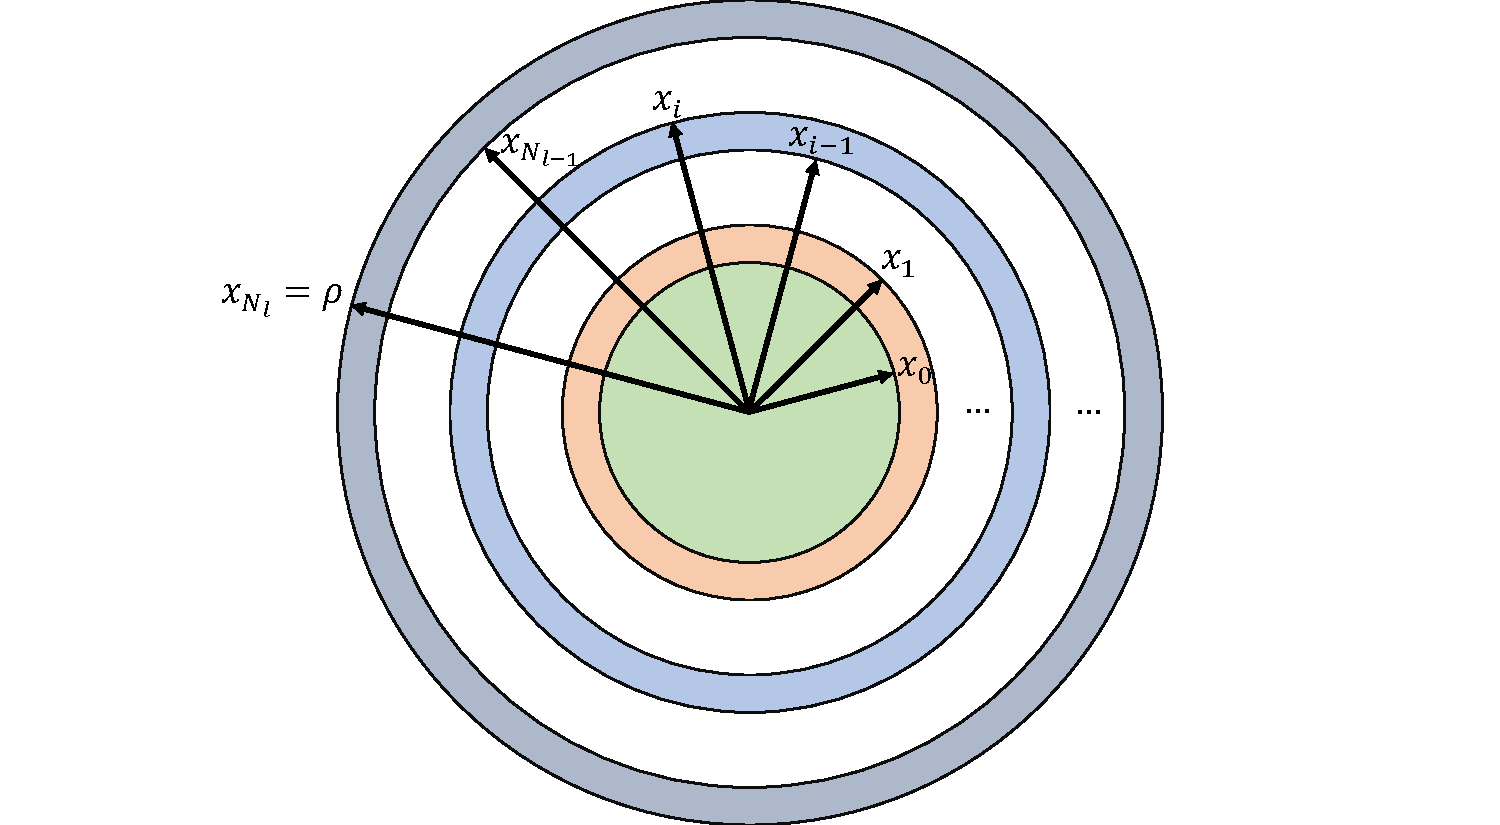
\includegraphics[width=0.8\textwidth]{./Figures/Sphere_Geometry.pdf}
\caption{\label{fig:Sphere_Geometry}Configuration of a layered sphere. The layered sphere is composed of a core and $N_{l}$ spherically symmetric layers. Each component of the sphere has an outer radius $x_{i}$ where $i=0$ for the core or $i$ takes the label of the layer, counting outward from the core. The radius of the outermost layer is also denoted $\rho$, to match the notation in the rest of this document.}
\end{figure}

%
The expressions for the effective Mie coefficients of uncoated and single-coating spheres are well known from the literature.\cite{Mie1976, Kaiser1993, Bohren2004, Zhou2006, Zheng2015} The full, multilayered Mie coefficients can be determined recursively in a manner similar to that of Fresnel reflection coefficients for planar stratified media.\cite{Narayanaswamy2013b} The recurrence relation is given by
%
\begin{subequations} \label{eq:MultilayeredMie}
\begin{align}
\widetilde{R}_{n}^{(M)}(x_{i}) &= \frac{ R_{n}^{(M)}(x_{i}) + \widetilde{R}_{n}^{(M)}(x_{i-1}) \alpha_{n}^{(M)}(x_{i}) }{ 1 + \widetilde{R}_{n}^{(M)}(x_{i-1}) \beta_{n}^{(M)}(x_{i}) }
\\
\widetilde{R}_{n}^{(N)}(x_{i}) &= \frac{ R_{n}^{(N)}(x_{i}) + \widetilde{R}_{n}^{(N)}(x_{i-1}) \alpha_{n}^{(N)}(x_{i}) }{ 1 + \widetilde{R}_{n}^{(N)}(x_{i-1}) \beta_{n}^{(N)}(x_{i}) }
\end{align}
\end{subequations}
%
where
%
\begin{subequations}\label{eq:Mie_definition1}
\begin{align}
R_{n}^{(M)}(x_{i})
&= - \frac{z_{n}^{(1)}(k_{i+1} x_{i})}{z_{n}^{(3)}(k_{i+1} x_{i})}
\left[ \frac{ \frac{1}{Z_{i+1}} \frac{\zeta_{n}^{(1)}(k_{i+1} x_{i})}{z_{n}^{(1)}(k_{i+1} x_{i})} - \frac{1}{Z_{i}} \frac{\zeta_{n}^{(1)}(k_{i} x_{i})}{z_{n}^{(1)}(k_{i} x_{i})} }{ \frac{1}{Z_{i+1}} \frac{\zeta_{n}^{(3)}(k_{i+1} x_{i})}{z_{n}^{(3)}(k_{i+1} x_{i})} - \frac{1}{Z_{i}} \frac{\zeta_{n}^{(1)}(k_{i} x_{i})}{z_{n}^{(1)}(k_{i} x_{i})} } \right]
\\
R_{n}^{(N)}(x_{i})
&= - \frac{\zeta_{n}^{(1)}(k_{i+1} x_{i})}{\zeta_{n}^{(3)}(k_{i+1} x_{i})}
\left[ \frac{ \frac{1}{Z_{i+1}} \frac{z_{n}^{(1)}(k_{i+1} x_{i})}{\zeta_{n}^{(1)}(k_{i+1} x_{i})} - \frac{1}{Z_{i}} \frac{z_{n}^{(1)}(k_{i} x_{i})}{\zeta_{n}^{(1)}(k_{i} x_{i})} }{ \frac{1}{Z_{i+1}} \frac{z_{n}^{(3)}(k_{i+1} x_{i})}{\zeta_{n}^{(3)}(k_{i+1} x_{i})} - \frac{1}{Z_{i}} \frac{z_{n}^{(1)}(k_{i} x_{i})}{\zeta_{n}^{(1)}(k_{i} x_{i})} } \right]
\end{align}
\end{subequations}
%
\begin{subequations}
\begin{align}
\alpha_{n}^{(M)}(x_{i})
&= - \frac{z_{n}^{(1)}(k_{i+1} x_{i})}{z_{n}^{(3)}(k_{i+1} x_{i})} \frac{z_{n}^{(3)}(k_{i} x_{i})}{z_{n}^{(1)}(k_{i} x_{i})}
\left[ \frac{ \frac{1}{Z_{i+1}} \frac{\zeta_{n}^{(1)}(k_{i+1} x_{i})}{z_{n}^{(1)}(k_{i+1} x_{i})} - \frac{1}{Z_{i}} \frac{\zeta_{n}^{(3)}(k_{i} x_{i})}{z_{n}^{(3)}(k_{i} x_{i})} }{ \frac{1}{Z_{i+1}} \frac{\zeta_{n}^{(3)}(k_{i+1} x_{i})}{z_{n}^{(3)}(k_{i+1} x_{i})} - \frac{1}{Z_{i}} \frac{\zeta_{n}^{(1)}(k_{i} x_{i})}{z_{n}^{(1)}(k_{i} x_{i})} } \right]
\\
\alpha_{n}^{(N)}( x_{i})
&= - \frac{\zeta_{n}^{(1)}(k_{i+1} x_{i})}{\zeta_{n}^{(3)}(k_{i+1} x_{i})} \frac{\zeta_{n}^{(3)}(k_{i} x_{i})}{\zeta_{n}^{(1)}(k_{i} x_{i})}
\left[ \frac{ \frac{1}{Z_{i+1}} \frac{z_{n}^{(1)}(k_{i+1} x_{i})}{\zeta_{n}^{(1)}(k_{i+1} x_{i})} - \frac{1}{Z_{i}} \frac{z_{n}^{(3)}(k_{i} x_{i})}{\zeta_{n}^{(3)}(k_{i} x_{i})} }{ \frac{1}{Z_{i+1}} \frac{z_{n}^{(3)}(k_{i+1} x_{i})}{\zeta_{n}^{(3)}(k_{i+1} x_{i})} - \frac{1}{Z_{i}} \frac{z_{n}^{(1)}(k_{i} x_{i})}{\zeta_{n}^{(1)}(k_{i} x_{i})} } \right]
\end{align}
\end{subequations}
%
\begin{subequations}\label{eq:Mie_definition3}
\begin{align}
\beta_{n}^{(M)}( x_{i})
&= \frac{z_{n}^{(3)}(k_{i} x_{i})}{z_{n}^{(1)}(k_{i} x_{i})}
\left[ \frac{ \frac{1}{Z_{i+1}} \frac{\zeta_{n}^{(3)}(k_{i+1} x_{i})}{z_{n}^{(3)}(k_{i+1} x_{i})} - \frac{1}{Z_{i}} \frac{\zeta_{n}^{(3)}(k_{i} x_{i})}{z_{n}^{(3)}(k_{i} x_{i})} }{ \frac{1}{Z_{i+1}} \frac{\zeta_{n}^{(3)}(k_{i+1} x_{i})}{z_{n}^{(3)}(k_{i+1} x_{i})} - \frac{1}{Z_{i}} \frac{\zeta_{n}^{(1)}(k_{i} x_{i})}{z_{n}^{(1)}(k_{i} x_{i})} } \right]
\\
\beta_{n}^{(N)}( x_{i})
&= \frac{\zeta_{n}^{(3)}(k_{i} x_{i})}{\zeta_{n}^{(1)}(k_{i} x_{i})}
\left[ \frac{ \frac{1}{Z_{i+1}} \frac{z_{n}^{(3)}(k_{i+1} x_{i})}{\zeta_{n}^{(3)}(k_{i+1} x_{i})} - \frac{1}{Z_{i}} \frac{z_{n}^{(3)}(k_{i} x_{i})}{\zeta_{n}^{(3)}(k_{i} x_{i})} }{ \frac{1}{Z_{i+1}} \frac{z_{n}^{(3)}(k_{i+1} x_{i})}{\zeta_{n}^{(3)}(k_{i+1} x_{i})} - \frac{1}{Z_{i}} \frac{z_{n}^{(1)}(k_{i} x_{i})}{\zeta_{n}^{(1)}(k_{i} x_{i})} } \right]
\end{align}
\end{subequations}

In Eqs. (\ref{eq:Mie_definition1})-(\ref{eq:Mie_definition3}), $Z=Z_0 \sqrt{\mu/\varepsilon}$ is the electromagnetic impedance for a dielectric material and $Z_0=\sqrt{\mu_0/\varepsilon_0}$ is the impedance of free space. $k_{i}$ refers to the value of $k$ within the core ($i=0$), layer $i$ ($1<i\le N_{l}$), or in the free-space region $f$ ($i=N_{l}+1$). The recursion relation is terminated by $\widetilde{R}_{n}^{(M)}(x_{0}) = R_{n}^{(M)}(x_{0})$ and $\widetilde{R}_{n}^{(N)}(x_{0}) = R_{n}^{(N)}(x_{0})$. The the case of a homogeneous sphere can be recovered from the recursion relations if the core and layers all have the same optical properties. In that case, Eq. \ref{eq:MultilayeredMie} simply to
%
\begin{subequations}
\begin{align}
\widetilde{R}_{n}^{(M)}(\rho) &= R_{n}^{(M)}(\rho)
\\
\widetilde{R}_{n}^{(N)}(\rho) &= R_{n}^{(N)}(\rho)
\end{align}
\end{subequations} % Done X
\chapter[Solution to Linear System][Solution to Linear System]{Solution to Linear System} \label{ap:SolutionToLinearSystem}
%
At first glance, the coupled system of equations given by Eq. \ref{eq:ScatteredFieldEquations} is not simple to solve for the scattered field coefficients, $V_{l, \nu, m}^{X,Y,i,j}$. To clarify the necessary approach, we start by unpacking Eq. \ref{eq:ScatteredFieldEquations} into all the equations it provides. We fix values of $m$, $i$, and $j$ and generate equations from all possible combinations of $X=M$ or $N$, $Y = M$ or $N$. We obtain
%
\begin{subequations}
\begin{align}
V_{l, \nu, m}^{M,M,i,j}
- \sum_{p=1}^{N_{s}} \sum_{n = \widetilde{m}}^{\infty}
\left[ \begin{array}{r}
V_{l,n,m}^{M,M,p,j} \widetilde{R}_{n}^{(M)}(\rho_{p}) C_{n,\nu,m}^{M,M,i,p}
\\
+ V_{l,n,m}^{N,M,p,j} \widetilde{R}_{n}^{(N)}(\rho_{p}) C_{n,\nu,m}^{M,N,i,p}
\end{array} \right]
&= C_{l, \nu, m}^{M,M,i,j}
\\
V_{l, \nu, m}^{N,M,i,j}
- \sum_{p=1}^{N_{s}} \sum_{n = \widetilde{m}}^{\infty}
\left[ \begin{array}{r}
V_{l,n,m}^{M,M,p,j} \widetilde{R}_{n}^{(M)}(\rho_{p}) C_{n,\nu,m}^{N,M,i,p}
\\
+ V_{l,n,m}^{N,M,p,j} \widetilde{R}_{n}^{(N)}(\rho_{p}) C_{n,\nu,m}^{N,N,i,p}
\end{array} \right]
&= C_{l, \nu, m}^{N,M,i,j}
\\
V_{l, \nu, m}^{M,N,i,j}
- \sum_{p=1}^{N_{s}} \sum_{n = \widetilde{m}}^{\infty}
\left[ \begin{array}{r}
V_{l,n,m}^{M,N,p,j} \widetilde{R}_{n}^{(M)}(\rho_{p}) C_{n,\nu,m}^{M,M,i,p}
\\
+ V_{l,n,m}^{N,N,p,j} \widetilde{R}_{n}^{(N)}(\rho_{p}) C_{n,\nu,m}^{M,N,i,p}
\end{array} \right]
& = C_{l, \nu, m}^{M,N,i,j}
\\
V_{l, \nu, m}^{N,N,i,j}
- \sum_{p=1}^{N_{s}} \sum_{n = \widetilde{m}}^{\infty}
\left[ \begin{array}{r}
V_{l,n,m}^{M,N,p,j} \widetilde{R}_{n}^{(M)}(\rho_{p}) C_{n,\nu,m}^{N,M,i,p}
\\
+ V_{l,n,m}^{N,N,p,j} \widetilde{R}_{n}^{(N)}(\rho_{p}) C_{n,\nu,m}^{N,N,i,p}
\end{array} \right]
& = C_{l, \nu, m}^{N,N,i,j}
\end{align}
\end{subequations}

In order to solve the linear system numerically, we must truncate the infinite sum to a finite number of terms, which we will denote $N_{\mathrm{max}}$. Additionally, we define $N_{\mathrm{terms}} = N_{\mathrm{max}} - \widetilde{m} + 1$. Now, we define four $N_{\mathrm{terms}} \times N_{\mathrm{terms}}$ matrices of scattered field coefficients: $\overline{\overline{\boldsymbol{V}}}_{m}^{M,M,i,j}$, $\overline{\overline{\boldsymbol{V}}}_{m}^{M,N,i,j}$, $\overline{\overline{\boldsymbol{V}}}_{m}^{N,M,i,j}$, and $\overline{\overline{\boldsymbol{V}}}_{m}^{N,N,i,j}$. Each element in the matrices is a value of $V_{l, \nu, m}^{X,Y,i,j}$ with $l \in [\widetilde{m}, N_{\mathrm{max}}]$ and $\nu \in [\widetilde{m}, N_{\mathrm{max}}]$. The $l$ index increases across rows, and $\nu$ increases down columns. For example, for $m=0$ and $N_{\mathrm{max}}=2$
%
\begin{equation}
\overline{\overline{\boldsymbol{V}}}_{m=0}^{X,Y,i,j} = \left[ \begin{array}{ccc}
V_{l=1, \nu=1, m=0}^{X,Y,i,j} & V_{l=2, \nu=1, m=0}^{X,Y,i,j} \\
V_{l=1, \nu=2, m=0}^{X,Y,i,j} & V_{l=2, \nu=2, m=0}^{X,Y,i,j}
\end{array}\right]
\end{equation}

Next we define a $(2 N_{\mathrm{terms}}) \times (2 N_{\mathrm{terms}})$ block matrix of coefficients for a given pair of spheres
\begin{equation}
\overline{\overline{\boldsymbol{V}}}_{m}^{i,j} = \left[ \begin{array}{c|c}
\overline{\overline{\boldsymbol{V}}}_{m}^{M,M,i,j} & \overline{\overline{\boldsymbol{V}}}_{m}^{M,N,i,j} \\ \hline
\overline{\overline{\boldsymbol{V}}}_{m}^{N,M,i,j} & \overline{\overline{\boldsymbol{V}}}_{m}^{N,N,i,j}
\end{array}\right]
\end{equation}
%
and an even greater $(2 N_{s} N_{\mathrm{terms}}) \times (2 N_{s} N_{\mathrm{terms}})$ block matrix for all pairs of spheres, $\overline{\overline{\boldsymbol{V}}}_{m}$, where the rows of the block matrix have increasing values of $i$ and the rows have increasing values of $j$. For example, for a two sphere system
\begin{equation}
\overline{\overline{\boldsymbol{V}}}_{m} = \left[ \begin{array}{c|c}
\overline{\overline{\boldsymbol{V}}}_{m}^{i=1,j=1} & \overline{\overline{\boldsymbol{V}}}_{m}^{i=1,j=2} \\ \hline
\overline{\overline{\boldsymbol{V}}}_{m}^{i=2,j=1} & \overline{\overline{\boldsymbol{V}}}_{m}^{i=2,j=2}
\end{array}\right]
\end{equation}

Now that the organization of the scattered field coefficients is clear, we move on to the organization of the Mie coefficients. Define a column vector, $\boldsymbol{R}^{j}_{\nu}$, whose entries are $\widetilde{R}^{(M)}_{\nu}(\rho_{j})$ and then $\widetilde{R}^{(M)}_{\nu}(\rho_{j})$, appended together. Only terms for which $\nu \in [\widetilde{m}, N_{\mathrm{max}}]$ are included. For example, for $m=0$ and $N_{\mathrm{max}}=2$
\begin{equation}
\boldsymbol{R}^{j}_{m=0} = \left[ \begin{array}{c}
\widetilde{R}^{(M)}_{\nu=1}(\rho_{j}) \\
\widetilde{R}^{(M)}_{\nu=2}(\rho_{j}) \\ \hline
\widetilde{R}^{(N)}_{\nu=1}(\rho_{j}) \\
\widetilde{R}^{(N)}_{\nu=2}(\rho_{j})
\end{array}\right]
\end{equation}

Next, define a Mie coefficient matrix
\begin{equation}
\overline{\overline{\boldsymbol{R}}}_{m} =\overline{\overline{\boldsymbol{I}}} \left[ \begin{array}{c}
\boldsymbol{R}^{j=1}_{m} \\ \hline
\boldsymbol{R}^{j=2}_{m} \\ \hline
\vdots \\ \hline
\boldsymbol{R}^{j=N_{\mathrm{s}}}_{m}
\end{array}\right]
\end{equation}
%
where $\overline{\overline{\boldsymbol{I}}}$ is an identity matrix with dimensions $(2 N_{s} N_{\mathrm{terms}}) \times (2 N_{s} N_{\mathrm{terms}})$.

The vector addition translation coefficients are first organized into $N_{\mathrm{terms}} \times N_{\mathrm{terms}}$ matrices. Each element in the matrices is a value of the translation coefficient with $l \in [\widetilde{m}, N_{\mathrm{max}}]$ and $\nu \in [\widetilde{m}, N_{\mathrm{max}}]$. The $l$ index increases across rows, and $\nu$ increases down columns. For example, given a pair of spheres $i$ and $j$ and for $m=0$ and $N_{\mathrm{max}}=2$
%
\begin{equation}
\overline{\overline{\boldsymbol{C}}}_{m=0}^{X,Y,i,j} = \left[ \begin{array}{cc}
C_{l=1,\nu=1,m=0}^{X,Y,i,j} & C_{l=2,\nu=1,m=0}^{X,Y,i,j} \\
C_{l=1,\nu=2,m=0}^{X,Y,i,j} & C_{l=2,\nu=2,m=0}^{X,Y,i,j}
\end{array}\right]
\end{equation}

Next we define a $(2 N_{\mathrm{terms}}) \times (2 N_{\mathrm{terms}})$ block matrix of coefficients for a given pair of spheres
\begin{equation}
\overline{\overline{\boldsymbol{C}}}_{m}^{i,j} = \left[ \begin{array}{c|c}
\overline{\overline{\boldsymbol{C}}}_{m}^{M,M,i,j} & \overline{\overline{\boldsymbol{C}}}_{m}^{M,N,i,j} \\ \hline
\overline{\overline{\boldsymbol{C}}}_{m}^{N,M,i,j} & \overline{\overline{\boldsymbol{C}}}_{m}^{N,N,i,j}
\end{array}\right]
\end{equation}
%
and an even greater $(2 N_{s} N_{\mathrm{terms}}) \times (2 N_{s} N_{\mathrm{terms}})$ block matrix for all pairs of spheres, $\overline{\overline{\boldsymbol{C}}}_{m}$, where the rows of the block matrix have increasing values of $i$ and the rows have increasing values of $j$. For example, for a two sphere system
\begin{equation}
\overline{\overline{\boldsymbol{C}}}_{m} = \left[ \begin{array}{c|c}
\overline{\overline{\boldsymbol{C}}}_{m}^{i=1,j=1} & \overline{\overline{\boldsymbol{C}}}_{m}^{i=1,j=2} \\ \hline
\overline{\overline{\boldsymbol{C}}}_{m}^{i=2,j=1} & \overline{\overline{\boldsymbol{C}}}_{m}^{i=2,j=2}
\end{array}\right]
\end{equation}

It is good to note here that, due to the definition of $C_{l, \nu, m}^{X,Y,i,j}$ in Eq. \ref{eq:TranslationCoefficients}, all the matrices on the main diagonal of $\overline{\overline{\boldsymbol{C}}}_{m}$ are identically zero.

The solution to the  linear system is given by
\begin{equation}\label{eq:LinearSystem_Matrix}
\begin{split}
\overline{\overline{\boldsymbol{V}}}_{m} &= \overline{\overline{\boldsymbol{R}}}_{m}^{-1} \left[ \overline{\overline{\boldsymbol{I}}} - \overline{\overline{\boldsymbol{R}}}_{m} \overline{\overline{\boldsymbol{C}}}_{m} \right]^{-1} \overline{\overline{\boldsymbol{R}}}_{m} \overline{\overline{\boldsymbol{C}}}_{m}
\\
&= \left[ \overline{\overline{\boldsymbol{I}}} - \overline{\overline{\boldsymbol{C}}}_{m} \overline{\overline{\boldsymbol{R}}}_{m} \right]^{-1} \overline{\overline{\boldsymbol{C}}}_{m}
\end{split}
\end{equation}

The second line of Eq. \ref{eq:LinearSystem_Matrix} is the most compact solution for the unknown scattered field coefficients, as defined in this work. The first line is presented in recognition of the fact that other works on light scattering by spheres sometimes define their scattered field coefficients proportional to $\overline{\overline{\boldsymbol{R}}}_{m} \overline{\overline{\boldsymbol{V}}}_{m}$ \cite{Narayanaswamy2008, Mackowski2008}. % Done X
\chapter[Basics of SCUFF-EM Software][Basics of SCUFF-EM Software]{Basics of SCUFF-EM Software} \label{ap:SCUFFEM}

\section{Introduction}
%
In this appendix, instructions are provided to perform NFRHT simulations using \textsc{scuff-em}, which is short for Surface CUrrent/Field Formulation of ElectroMagnetism. \textsc{scuff-em} is a free, open-source software implementation of the boundary-element method \cite{scuffem, Reid2015} which models fluctuating-surface-currents as the source of thermal radiation. The source code for \textsc{scuff-em} is available at \url{https://github.com/HomerReid/scuff-em/}.

Instructions will be provided assuming installation on a computer running Ubuntu 14.04 locally. Some modification may be required when using other systems. These instructions are meant to be supplemental to the existing \href{http://homerreid.github.io/scuff-em-documentation/}{\textsc{scuff-em} documentation} and will not cover all features of the software. They will, however, cover all steps required to perform the NFRHT calculations completed in this dissertation. Broadly speaking, there are three main steps: (1) Create and mesh each object. (2) Define the configuration of all objects. (3) Feed the appropriate files to \textsc{scuff-em} to run a simulation. These steps are described below.


\section{Creating the Mesh}
%
\textsc{scuff-em} requires meshed surfaces, and the free software \href{http://gmsh.info/}{Gmsh} is recommended to create the meshes. The first step is to create a Gmsh geometry file for each unique object. For a sphere, such a file looks like Listing \ref{lst:GmshGeometry}. The value of $R$ given in line 8 should be given in micrometers. The meshing finenesses given in lines 13-15 should be adjusted depending on the geometry being investigated. For a uniform mesh, set $l1=l2=l3$. In this appendix, I will show an example for NFRHT between two spheres. In that situation, it is advantageous for increase the density of the mesh at a single pole only, in this case the north pole. The point, circle, line loop, ruled surface, and physical surface commands on lines 20-55 are used to build a boundary representation of a sphere from primitive objects like points and arcs. For further information, I direct readers to the \href{http://gmsh.info/doc/texinfo/gmsh.html}{Gmsh documentation}. The file given in Listing \ref{lst:GmshGeometry} may be used for any sphere by altering the values on lines 8, 13, 14, and 15.

\singlespacing
\begin{lstlisting}[language=C++, caption={Gmsh geometry file for a sphere.}, label={lst:GmshGeometry}]
//
// Gmsh geometry specification for a sphere of radius R
// 

//************************************************************
//* input parameters      
//************************************************************
R = 10.0;    // radius

//************************************************************
//* meshing finenesses ***************************************
//************************************************************
l3 = 0.10;  // fineness at north pole
l2 = 1.00;  // fineness at equator
l1 = 1.00;  // fineness at south pole

//************************************************************
//* defintion of sphere *********************************************
//************************************************************
Point(1) = {  0 ,    0,  0.0,  l2};
Point(2) = {  R,    0,  0.0,  l2};
Point(3) = {  0 ,   R,  0.0,  l2};
Circle(1) = {2,1,3};
Point(4) = { -R,    0,  0.0,  l2};
Point(5) = {   0,  -R,  0.0,  l2};
Circle(2) = {3,1,4};
Circle(3) = {4,1,5};
Circle(4) = {5,1,2};
Point(6) = {   0,    0,  0.0+R, l3};
Point(7) = {   0,    0,  0.0-R, l1};
Circle(5) = {3,1,6};
Circle(6) = {6,1,5};
Circle(7) = {5,1,7};
Circle(8) = {7,1,3};
Circle(9) = {2,1,7};
Circle(10) = {7,1,4};
Circle(11) = {4,1,6};
Circle(12) = {6,1,2};
Line Loop(13) = {2,8,-10};
Ruled Surface(14) = {13};
Line Loop(15) = {10,3,7};
Ruled Surface(16) = {15};
Line Loop(17) = {-8,-9,1};
Ruled Surface(18) = {17};
Line Loop(19) = {-11,-2,5};
Ruled Surface(20) = {19};
Line Loop(21) = {-5,-12,-1};
Ruled Surface(22) = {21};
Line Loop(23) = {-3,11,6};
Ruled Surface(24) = {23};
Line Loop(25) = {-7,4,9};
Ruled Surface(26) = {25};
Line Loop(27) = {-4,12,-6};
Ruled Surface(28) = {27};
Physical Surface(1) = {28,26,16,14,20,24,22,18};

//************************************************************
//* reference point to get outward-pointing surface normals right
//************************************************************
Physical Point(1) = {1};
\end{lstlisting}
\doublespacing

Next, Gmsh must be used to generate a mesh file from the geometry file. This can be done through the terminal window. If the geometry file given in Listing \ref{lst:GmshGeometry} is saved as Geometry.geo in the current working directory, a mesh file, called Mesh.msh, is generated by the command
%
\begin{lstlisting}[language=C++]
gmsh -2 -clscale 5.0 Geometry.geo -format msh2 -o Mesh.msh
\end{lstlisting}
%
where the -clscale parameter controls the fineness of the mesh. Its value can be decreased to create a finer mesh, or increased to create a less dense mesh. The same mesh may be used for two identical objects; separate mesh files must be generated for any unique objects.  


\section{Defining the Configuration}
%
Now that the mesh file has been created, the \textsc{scuff-em} geometry file is next. \textsc{scuff-em} geometry files carry the extension .scuffgeo and define the orientation, location, mesh file, and optical properties of each object. An example of a \textsc{scuff-em} geometry file is given in Listing \ref{lst:SCUFFGeometry} for two silicon dioxide spheres separated by a center-to-center distance of 15 \si{\micro\meter}.

\singlespacing
\begin{lstlisting}[language=Perl, caption={\textsc{scuff-em} geometry file.}, label={lst:SCUFFGeometry}]
# dielectric model for silicon dioxide
MATERIAL SIO2
	A1 = 8.2736e+13;
 	w01 = 8.54484e+13;
 	G1 = 8.46448e+12;
 	A2 = 1.58004e+14;
 	w02 = 2.029e+14;
 	G2 = 1.06449e+13;
 	A3 = 3.39786e+13;
 	w03 = 1.51198e+14;
 	G3 = 8.33205e+12;
 	EpsInf = 2.03843;
 
 	Eps(w) = EpsInf + A1*A1/(w01*w01 - w*w - i*w*G1) + A2*A2/(w02*w02 - w*w - i*w*G2) + A3*A3/(w03*w03 - w*w - i*w*G3);
ENDMATERIAL

OBJECT Sphere1
	MESHFILE Mesh.msh
	MATERIAL SIO2
ENDOBJECT

OBJECT Sphere2
	MESHFILE Mesh.msh
	MATERIAL SIO2
	ROTATED 180 ABOUT 1 0 0
	DISPLACED 0 0 25.0
ENDOBJECT
\end{lstlisting}
\doublespacing

There are two main components to the \textsc{scuff-em} geometry file: material declarations and object declarations. Material declarations provide the dielectric function of a given material and should appear first in a \textsc{scuff-em} geometry file. Multiple materials may be defined sequentially. Advanced users may also choose to locate their material declarations in a central repository. \textsc{scuff-em} has two built-in materials: vacuum and perfect electrical conductor (PEC). The dielectric function must be calculated in units of $u = \omega/\omega_{0}$ where $\omega_{0} = 3 \times 10^{14}$ \si{\radian\per\second}. To convert from wavelength $\lambda$ (in micrometers) to $u$, use $\lambda = 2\pi/u$

Object declarations are used for finite objects, bounded by finite surfaces, which are not touching any other objects. They specify the mesh file, material, and configuration using the MESHFILE, MATERIAL, and ROTATED/DISPLACED keywords, respectively. MESHFILE refers to a previously created mesh, which should be stored in the current working directory or in a central repository. MATERIAL refers to the previously discussed material declaration. Failure to provide MATERIAL results in an object being treated as a PEC. ROTATED refers to the orientation of the object's intrinsic coordinate axes relative to the global axes. ROTATED has arguments $d$ ABOUT $ax$ $ay$ $az$, where $d$ is the rotation (in degrees) and $ax$, $ay$, $az$ correspond to the $x$, $y$, and $z$-axes. The ROTATED command in Listing \ref{lst:SCUFFGeometry} produces a rotation about the $x$-axis of 180 degrees. DISPLACED refers to the Cartesian translation of an object's intrinsic origin relative to the global coordinate system's origin. For the sphere defined above, the intrinsic origin lies at the sphere's center. Failure to provide values for DISPLACED results in the object's axes and origin to be aligned with a global set of axes and a global origin. The DISPLACED keyword takes three arguments: $x$ $y$ $z$. For example in Listing \ref{lst:SCUFFGeometry}, Sphere2 is translated 25 \si{\micro\meter} in the positive z-direction. Since Sphere1 and Sphere2 have radii of 10 \si{\micro\meter}, they are separated by a minimum separation distance of 5 \si{\micro\meter}. The ROTATED and DISPLACED commands are read sequentially, so care must be taken to ensure they are given in the intended order. For example, if lines 25 (ROTATED) and 26 (DISPLACED) are reversed in Listing \ref{lst:SCUFFGeometry}, the translation and rotation of Sphere2 will result in its origin being located at $(0,0,-25)$ instead of $(0,0,25)$. 

It is important to note that there are many other more advanced features which may be included in a \textsc{scuff-em} geometry file. I direct readers to \url{http://homerreid.github.io/scuff-em-documentation/reference/Geometries/} for further details.

Once a \textsc{scuff-em} geometry file is created, I advise visually checking the resulting geometry using Gmsh. To do so, use the terminal command
%
\begin{lstlisting}[language=C++]
scuff-analyze --geometry Geometry.scuffgeo --WriteGMSHFiles
\end{lstlisting}
%
and then open the resulting file with the extension .pp using Gmsh. For the example presented above, the result is shown in Fig. \ref{fig:SCUFF_Visualization}. The bottom sphere is Sphere1 and the top sphere is Sphere2. Sphere1 clearly shows the denser mesh at its northern pole; the underside of Sphere2 is identical.

\begin{figure}
\centering
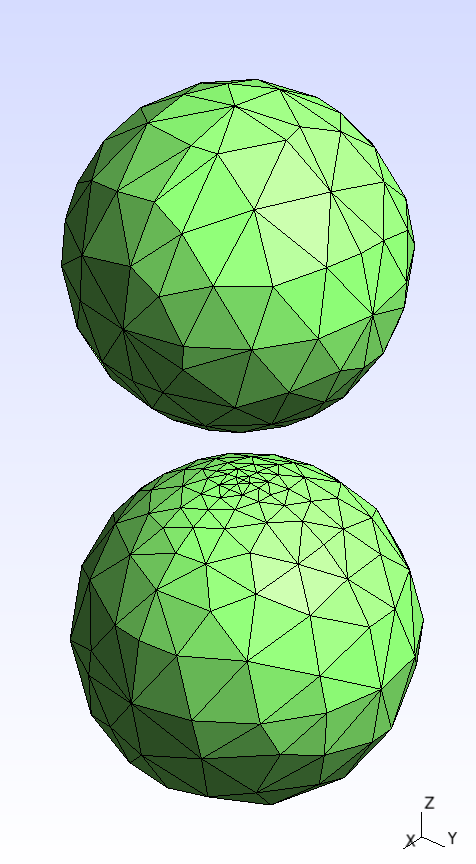
\includegraphics[width=0.35\textwidth]{./Figures/SCUFF_Visualization.png}
\caption{\label{fig:SCUFF_Visualization}Visualization of the \textsc{scuff-em} geometry file, created using Gmsh.}
\end{figure}


\section{Running a Simulation}
%
To run a single NFRHT simulation, we will call upon the code for non-equilibrium (NEQ) fluctuation-induced phenomena. It can handle both NFRHT and Casimir force calculations. We are interested in calculating the transmissivity function between objects. In the parlance of SCUFF-EM, it is called the generalized flux, $\Phi_{s \rightarrow d}(u)$. The generalized flux output by SCUFF-EM is exactly equal to $\tau_{s \rightarrow d}(\omega)$ from Eq. \ref{eq:NetHeatTransfer}. The command to compute NFRHT is
%
\begin{lstlisting}[language=C++]
scuff-neq --geometry Geometry.scuffgeo --OmegaFile OmegaFile
\end{lstlisting}
%
where OmegaFile is a file of values of $u$ at which $\Phi_{s \rightarrow d}(u)$ will be evaluated. Each value of $u$ in OmegaFile should occupy its own line. The example showed is the most basic NFRHT calculation. Several customizations are available, and I direct readers to \url{http://homerreid.github.io/scuff-em-documentation/applications/scuff-neq/scuff-neq/} for all of them.

There is one special option to which I will draw attention: transformations. Many elements of the scattering matrix used to compute NFRHT require properties of the individual bodies alone, and thus can be reused if a heat transfer-distance is desired. In order to save computational time, a transformation file can be supplied which details all the translations (or rotations) desired. The transformation file should give all translations and rotations relative to the configuration given in the \textsc{scuff-em} geometry file. For example, a file which takes our spheres and also computes NFRHT with minimum separation gaps of 10, 15, and 20 \si{\micro\meter} would read

\singlespacing
\begin{lstlisting}[language=Perl, caption={\textsc{scuff-em} transformation file.}, label={lst:SCUFFTransformation}]
TRANS 5  OBJECT Sphere2 DISP 0 0  0
TRANS 10 OBJECT Sphere2 DISP 0 0  5
TRANS 15 OBJECT Sphere2 DISP 0 0  10
TRANS 20 OBJECT Sphere2 DISP 0 0  15
\end{lstlisting}
\doublespacing
%
where the second column is a label, the fourth column is the object being transformed, and the sixth, seventh, and eighth columns are the Cartesian translations (relative to the \textsc{scuff-em} geometry file). There are a number of more sophisticated transformation methods allowed, which are covered extensively in \url{http://homerreid.github.io/scuff-em-documentation/reference/Transformations/}. The command to execute a NFRHT simulation using a transformation file is

\singlespacing
\begin{lstlisting}[language=C++]
scuff-neq --geometry Geometry.scuffgeo --TransFile Transformation --OmegaFile OmegaFile
\end{lstlisting}
\doublespacing
%
where Transformation is the \textsc{scuff-em} transformation file.

The result of such a command is a file called Geometry.SIFlux.EMTPFT where SI refers to the result being spatially integrated and EMTPFT (energy-momentum transfer, power force torque) refers to the method of integration (EMTPFT is the default method). An example output file is given in Listing \ref{lst:SCUFFExampleResults} for two objects and two frequencies. The columns of the file are the (1) transformation label (0.0 if no transformation file is provided), (2) non-dimensional frequency $u$, (3) source and destination objects, (4) flux spectral density of absorbed power ($\Phi_{s \rightarrow d}$), (5) flux spectral density of radiated power, (6-8) $x$, $y$, and $z$ components of force flux spectral density, and (9-11) $x$, $y$, and $z$ components of torque flux spectral density.

\singlespacing
\begin{lstlisting}[language=Perl, caption=Sample output file from {\textsc{scuff-em}.}, label={lst:SCUFFExampleResults}]
# scuff-neq run on Lab127 (08/29/18::18:33:30)
# data file columns: 
# 1 transform tag
# 2 omega 
# 3 (sourceSurface,destSurface) 
# 4 PAbs flux spectral density
# 5 PRad flux spectral density
# 6 XForce flux spectral density
# 7 YForce flux spectral density
# 8 ZForce flux spectral density
# 9 XTorque flux spectral density
# 10 YTorque flux spectral density
# 11 ZTorque flux spectral density
0.0 1.256637e+00 11 -7.90281126e-03 +7.90281126e-03 +2.69890579e-09 +8.84873807e-09 +5.63661446e-06 +3.61864629e-07 -3.84970743e-07 +1.83454544e-07 
0.0 1.256637e+00 12 +3.13534531e-07 -3.13534531e-07 -2.31817174e-10 -8.73833724e-10 +3.15096081e-06 +7.15556954e-09 -1.58668386e-07 +3.72063847e-09 
0.0 1.256637e+00 21 +3.13534530e-07 -3.13534530e-07 +3.49548060e-10 +8.71691790e-10 -3.15110593e-06 -8.50545313e-09 -1.70369659e-08 +1.50823996e-09 
0.0 1.256637e+00 22 -7.90281156e-03 +7.90281156e-03 +3.03177834e-09 +8.33691980e-09 -5.65780382e-06 -8.43395835e-05 +3.44041141e-05 +1.84850281e-07 
0.0 1.231997e+00 11 -8.12161225e-03 +8.12161225e-03 +2.33929940e-09 +8.21665833e-09 -1.23062421e-06 +3.92032030e-07 -4.11282818e-07 +1.79000346e-07 
0.0 1.231997e+00 12 +3.44786515e-07 -3.44786515e-07 -2.21137091e-10 -8.30112384e-10 +2.79435617e-06 +4.43090059e-09 -1.52735690e-07 +3.57295128e-09 
0.0 1.231997e+00 21 +3.44786514e-07 -3.44786514e-07 +3.41479370e-10 +8.37460786e-10 -2.79450235e-06 +4.12857975e-09 -2.13249109e-08 -6.37395124e-10 
0.0 1.231997e+00 22 -8.12161250e-03 +8.12161250e-03 +2.99997828e-09 +7.74714497e-09 +1.21073213e-06 -8.33215031e-05 +3.39882913e-05 +1.82055594e-07
\end{lstlisting}
\doublespacing
%

For NFRHT calculations, columns 6 through 11 may be ignored. $\tau_{s \rightarrow d}(\omega)$, defined in Eq. \ref{eq:NetHeatTransfer}, is exactly equal to the value of $\Phi_{s \rightarrow d}(u)$ located in column 4 for $s \ne d$. $\tau_{s \rightarrow E}(\omega)$, the transmissivity function defined between an object and its environment, is not given directly by \textsc{SCUFF-EM}. Instead, it must be obtained using quantities from column 4 and 
\begin{equation}
\tau_{s \rightarrow E}(\omega) = -\sum_{\alpha} \Phi_{s \rightarrow \alpha}
\end{equation}
%
where $\alpha$ is an index over all objects, including $\alpha=s$. The self-contribution to the transmissivity is negative and has a large magnitude, so $\tau_{s \rightarrow E} > 0$. For an isolated object, $\tau_{s \rightarrow E} = \Phi_{s \rightarrow s}$.

\end{document}